\documentclass[a4paper]{book}
\usepackage{a4wide}
\usepackage{makeidx}
\usepackage{fancyhdr}
\usepackage{graphicx}
\usepackage{multicol}
\usepackage{float}
\usepackage{textcomp}
\usepackage{alltt}
\usepackage{times}
\usepackage{ifpdf}
\ifpdf
\usepackage[pdftex,
            pagebackref=true,
            colorlinks=true,
            linkcolor=blue,
            unicode
           ]{hyperref}
\else
\usepackage[ps2pdf,
            pagebackref=true,
            colorlinks=true,
            linkcolor=blue,
            unicode
           ]{hyperref}
\usepackage{pspicture}
\fi
\usepackage[utf8]{inputenc}
\usepackage{doxygen}
\makeindex
\setcounter{tocdepth}{3}
\renewcommand{\footrulewidth}{0.4pt}
\begin{document}
\begin{titlepage}
\vspace*{7cm}
\begin{center}
{\Large temperature sensor \\[1ex]\large Terciopelo }\\
\vspace*{1cm}
{\large Generated by Doxygen 1.5.7}\\
\vspace*{0.5cm}
{\small Thu Nov 20 14:52:48 2008}\\
\end{center}
\end{titlepage}
\clearemptydoublepage
\pagenumbering{roman}
\tableofcontents
\clearemptydoublepage
\pagenumbering{arabic}
\chapter{File Index}
\section{File List}
Here is a list of all files with brief descriptions:\begin{CompactList}
\item\contentsline{section}{/Users/nikki/nublabs/nub.datalogger/hardware/temperature\_\-sensor\_\-Terciopelo/\hyperlink{communications_8h}{communications.h} }{\pageref{communications_8h}}{}
\item\contentsline{section}{/Users/nikki/nublabs/nub.datalogger/hardware/temperature\_\-sensor\_\-Terciopelo/\hyperlink{communications__definitions_8h}{communications\_\-definitions.h} }{\pageref{communications__definitions_8h}}{}
\item\contentsline{section}{/Users/nikki/nublabs/nub.datalogger/hardware/temperature\_\-sensor\_\-Terciopelo/\hyperlink{globals_8h}{globals.h} }{\pageref{globals_8h}}{}
\item\contentsline{section}{/Users/nikki/nublabs/nub.datalogger/hardware/temperature\_\-sensor\_\-Terciopelo/\hyperlink{name_8h}{name.h} }{\pageref{name_8h}}{}
\item\contentsline{section}{/Users/nikki/nublabs/nub.datalogger/hardware/temperature\_\-sensor\_\-Terciopelo/\hyperlink{nublogger_8h}{nublogger.h} }{\pageref{nublogger_8h}}{}
\item\contentsline{section}{/Users/nikki/nublabs/nub.datalogger/hardware/temperature\_\-sensor\_\-Terciopelo/\hyperlink{temperature__sensor__board__v2_8h}{temperature\_\-sensor\_\-board\_\-v2.h} }{\pageref{temperature__sensor__board__v2_8h}}{}
\item\contentsline{section}{/Users/nikki/nublabs/nub.datalogger/hardware/temperature\_\-sensor\_\-Terciopelo/\hyperlink{temperature__sensor___terciopelo_8pde}{temperature\_\-sensor\_\-Terciopelo.pde} }{\pageref{temperature__sensor___terciopelo_8pde}}{}
\item\contentsline{section}{/Users/nikki/nublabs/nub.datalogger/hardware/temperature\_\-sensor\_\-Terciopelo/applet/\hyperlink{applet_2communications_8h}{communications.h} }{\pageref{applet_2communications_8h}}{}
\item\contentsline{section}{/Users/nikki/nublabs/nub.datalogger/hardware/temperature\_\-sensor\_\-Terciopelo/applet/\hyperlink{applet_2communications__definitions_8h}{communications\_\-definitions.h} }{\pageref{applet_2communications__definitions_8h}}{}
\item\contentsline{section}{/Users/nikki/nublabs/nub.datalogger/hardware/temperature\_\-sensor\_\-Terciopelo/applet/\hyperlink{applet_2globals_8h}{globals.h} }{\pageref{applet_2globals_8h}}{}
\item\contentsline{section}{/Users/nikki/nublabs/nub.datalogger/hardware/temperature\_\-sensor\_\-Terciopelo/applet/\hyperlink{applet_2name_8h}{name.h} }{\pageref{applet_2name_8h}}{}
\item\contentsline{section}{/Users/nikki/nublabs/nub.datalogger/hardware/temperature\_\-sensor\_\-Terciopelo/applet/\hyperlink{applet_2nublogger_8h}{nublogger.h} }{\pageref{applet_2nublogger_8h}}{}
\item\contentsline{section}{/Users/nikki/nublabs/nub.datalogger/hardware/temperature\_\-sensor\_\-Terciopelo/applet/\hyperlink{applet_2temperature__sensor__board__v2_8h}{temperature\_\-sensor\_\-board\_\-v2.h} }{\pageref{applet_2temperature__sensor__board__v2_8h}}{}
\item\contentsline{section}{/Users/nikki/nublabs/nub.datalogger/hardware/temperature\_\-sensor\_\-Terciopelo/applet/\hyperlink{temperature__sensor___terciopelo_8cpp}{temperature\_\-sensor\_\-Terciopelo.cpp} }{\pageref{temperature__sensor___terciopelo_8cpp}}{}
\item\contentsline{section}{/Users/nikki/nublabs/nub.datalogger/hardware/temperature\_\-sensor\_\-Terciopelo/applet/\hyperlink{applet_2temperature__sensor___terciopelo_8pde}{temperature\_\-sensor\_\-Terciopelo.pde} }{\pageref{applet_2temperature__sensor___terciopelo_8pde}}{}
\end{CompactList}

\chapter{File Documentation}
\hypertarget{applet_2communications_8h}{
\section{/Users/nikki/nublabs/nub.datalogger/hardware/temperature\_\-sensor\_\-Terciopelo/applet/communications.h File Reference}
\label{applet_2communications_8h}\index{/Users/nikki/nublabs/nub.datalogger/hardware/temperature\_\-sensor\_\-Terciopelo/applet/communications.h@{/Users/nikki/nublabs/nub.datalogger/hardware/temperature\_\-sensor\_\-Terciopelo/applet/communications.h}}
}
{\tt \#include $<$HardwareSerial.h$>$}\par
{\tt \#include $<$string.h$>$}\par


Include dependency graph for communications.h:

This graph shows which files directly or indirectly include this file:\subsection*{Functions}
\begin{CompactItemize}
\item 
int \hyperlink{applet_2communications_8h_f8c68e93feeba5b9244094043672bac0}{getByte} (int timeout)
\end{CompactItemize}


\subsection{Function Documentation}
\hypertarget{applet_2communications_8h_f8c68e93feeba5b9244094043672bac0}{
\index{applet/communications.h@{applet/communications.h}!getByte@{getByte}}
\index{getByte@{getByte}!applet/communications.h@{applet/communications.h}}
\subsubsection[{getByte}]{\setlength{\rightskip}{0pt plus 5cm}int getByte (int {\em timeout})}}
\label{applet_2communications_8h_f8c68e93feeba5b9244094043672bac0}




Definition at line 4 of file communications.h.

Referenced by discover(), and sendData().

\begin{Code}\begin{verbatim}5 {
6   int currentTime=millis();
7   int maxTime=currentTime+timeout;
8   while((Serial.available()==0)&&(millis()<(maxTime)))
9     {}
10   if((millis()>maxTime)||(Serial.available()==0))
11     return -1;
12   else
13     return Serial.read();
14 }
\end{verbatim}
\end{Code}



\hypertarget{communications_8h}{
\section{/Users/nikki/nublabs/nub.datalogger/hardware/temperature\_\-sensor\_\-Terciopelo/communications.h File Reference}
\label{communications_8h}\index{/Users/nikki/nublabs/nub.datalogger/hardware/temperature\_\-sensor\_\-Terciopelo/communications.h@{/Users/nikki/nublabs/nub.datalogger/hardware/temperature\_\-sensor\_\-Terciopelo/communications.h}}
}
{\tt \#include $<$HardwareSerial.h$>$}\par
{\tt \#include $<$string.h$>$}\par


Include dependency graph for communications.h:

This graph shows which files directly or indirectly include this file:\subsection*{Functions}
\begin{CompactItemize}
\item 
int \hyperlink{communications_8h_f8c68e93feeba5b9244094043672bac0}{getByte} (int timeout)
\end{CompactItemize}


\subsection{Function Documentation}
\hypertarget{communications_8h_f8c68e93feeba5b9244094043672bac0}{
\index{communications.h@{communications.h}!getByte@{getByte}}
\index{getByte@{getByte}!communications.h@{communications.h}}
\subsubsection[{getByte}]{\setlength{\rightskip}{0pt plus 5cm}int getByte (int {\em timeout})}}
\label{communications_8h_f8c68e93feeba5b9244094043672bac0}




Definition at line 4 of file communications.h.

Referenced by discover().

\begin{Code}\begin{verbatim}5 {
6   int currentTime=millis();
7   int maxTime=currentTime+timeout;
8   while((Serial.available()==0)&&(millis()<(maxTime)))
9     {}
10   if((millis()>maxTime)||(Serial.available()==0))
11     return -1;
12   else
13     return Serial.read();
14 }
\end{verbatim}
\end{Code}



\hypertarget{applet_2communications__definitions_8h}{
\section{/Users/nikki/nublabs/nub.datalogger/hardware/temperature\_\-sensor\_\-Terciopelo/applet/communications\_\-definitions.h File Reference}
\label{applet_2communications__definitions_8h}\index{/Users/nikki/nublabs/nub.datalogger/hardware/temperature\_\-sensor\_\-Terciopelo/applet/communications\_\-definitions.h@{/Users/nikki/nublabs/nub.datalogger/hardware/temperature\_\-sensor\_\-Terciopelo/applet/communications\_\-definitions.h}}
}


This graph shows which files directly or indirectly include this file:\subsection*{Defines}
\begin{CompactItemize}
\item 
\#define \hyperlink{applet_2communications__definitions_8h_1685ca2e434799fb98ea9272ed39d5e3}{NUM\_\-TRIES}~1
\item 
\#define \hyperlink{applet_2communications__definitions_8h_d97232eed56f4b8962167188db8dd2d4}{ACKNOWLEDGE}~1
\begin{CompactList}\small\item\em these are defined messages sent between the sensor and the computer \item\end{CompactList}\item 
\#define \hyperlink{applet_2communications__definitions_8h_421ea5726b2e7e3464457785964b3c11}{ACKNOWLEDGE\_\-AND\_\-CONFIGURE}~2
\item 
\#define \hyperlink{applet_2communications__definitions_8h_29d0028b064fb993c0e1f2b1ce4a7f88}{LISTENING}~3
\item 
\#define \hyperlink{applet_2communications__definitions_8h_d7285ac8b394b259876f0e61574dd8b0}{CHECKSUM\_\-ERROR\_\-PLEASE\_\-RESEND}~4
\item 
\#define \hyperlink{applet_2communications__definitions_8h_b111ad1c600abfe6a9a3a7e7a1a057d5}{CHECKSUM\_\-ERROR\_\-GIVING\_\-UP}~5
\item 
\#define \hyperlink{applet_2communications__definitions_8h_9413ad5afdb7d48c2d8606409cde00d0}{DISCOVER\_\-ME}~6
\item 
\#define \hyperlink{applet_2communications__definitions_8h_efc48d416c882f06edaf6d01779d4d74}{TIMEOUT\_\-ERROR}~7
\item 
\#define \hyperlink{applet_2communications__definitions_8h_c4da90313e5d11e20acac66663fb014c}{MALFORMED\_\-MESSAGE\_\-ERROR\_\-PLEASE\_\-RESEND}~8
\item 
\#define \hyperlink{applet_2communications__definitions_8h_bf39c03638711128272afb73031f864d}{MALFORMED\_\-MESSAGE\_\-ERROR\_\-GIVING\_\-UP}~9
\item 
\#define \hyperlink{applet_2communications__definitions_8h_53b51d504d04d1bbfb3d4a4f57349480}{MESSAGE\_\-START}~128
\item 
\#define \hyperlink{applet_2communications__definitions_8h_012714d5d0e7065e355fefe979491541}{MESSAGE\_\-END}~129
\item 
\#define \hyperlink{applet_2communications__definitions_8h_d82632844d46de002b8d8d16900e42a0}{HOUR\_\-HIGH}~1
\item 
\#define \hyperlink{applet_2communications__definitions_8h_3faa4fcb5d61433ccf65f19b4de44703}{HOUR\_\-LOW}~2
\item 
\#define \hyperlink{applet_2communications__definitions_8h_592fee6a2134a20e8761668cb7c773e3}{MINUTE\_\-HIGH}~3
\item 
\#define \hyperlink{applet_2communications__definitions_8h_2ace92e75321bdd463da760570b4e7e7}{MINUTE\_\-LOW}~4
\item 
\#define \hyperlink{applet_2communications__definitions_8h_f4364f097130bbbe71669acfee2692ae}{SECOND\_\-HIGH}~5
\item 
\#define \hyperlink{applet_2communications__definitions_8h_15e121356786cb610493f80e4b35e677}{SECOND\_\-LOW}~6
\item 
\#define \hyperlink{applet_2communications__definitions_8h_9886586c91a412164c69eb0270d2875e}{CHECKSUM}~7
\item 
\#define \hyperlink{applet_2communications__definitions_8h_8ec36de1ede672b53100e0414d57a75a}{CONFIGURATION\_\-MESSAGE\_\-LENGTH}~8
\end{CompactItemize}


\subsection{Define Documentation}
\hypertarget{applet_2communications__definitions_8h_d97232eed56f4b8962167188db8dd2d4}{
\index{applet/communications\_\-definitions.h@{applet/communications\_\-definitions.h}!ACKNOWLEDGE@{ACKNOWLEDGE}}
\index{ACKNOWLEDGE@{ACKNOWLEDGE}!applet/communications_definitions.h@{applet/communications\_\-definitions.h}}
\subsubsection[{ACKNOWLEDGE}]{\setlength{\rightskip}{0pt plus 5cm}\#define ACKNOWLEDGE~1}}
\label{applet_2communications__definitions_8h_d97232eed56f4b8962167188db8dd2d4}


these are defined messages sent between the sensor and the computer 



Definition at line 9 of file communications\_\-definitions.h.

Referenced by discover(), and sendData().\hypertarget{applet_2communications__definitions_8h_421ea5726b2e7e3464457785964b3c11}{
\index{applet/communications\_\-definitions.h@{applet/communications\_\-definitions.h}!ACKNOWLEDGE\_\-AND\_\-CONFIGURE@{ACKNOWLEDGE\_\-AND\_\-CONFIGURE}}
\index{ACKNOWLEDGE\_\-AND\_\-CONFIGURE@{ACKNOWLEDGE\_\-AND\_\-CONFIGURE}!applet/communications_definitions.h@{applet/communications\_\-definitions.h}}
\subsubsection[{ACKNOWLEDGE\_\-AND\_\-CONFIGURE}]{\setlength{\rightskip}{0pt plus 5cm}\#define ACKNOWLEDGE\_\-AND\_\-CONFIGURE~2}}
\label{applet_2communications__definitions_8h_421ea5726b2e7e3464457785964b3c11}




Definition at line 10 of file communications\_\-definitions.h.

Referenced by discover(), and sendData().\hypertarget{applet_2communications__definitions_8h_9886586c91a412164c69eb0270d2875e}{
\index{applet/communications\_\-definitions.h@{applet/communications\_\-definitions.h}!CHECKSUM@{CHECKSUM}}
\index{CHECKSUM@{CHECKSUM}!applet/communications_definitions.h@{applet/communications\_\-definitions.h}}
\subsubsection[{CHECKSUM}]{\setlength{\rightskip}{0pt plus 5cm}\#define CHECKSUM~7}}
\label{applet_2communications__definitions_8h_9886586c91a412164c69eb0270d2875e}




Definition at line 29 of file communications\_\-definitions.h.

Referenced by configure().\hypertarget{applet_2communications__definitions_8h_b111ad1c600abfe6a9a3a7e7a1a057d5}{
\index{applet/communications\_\-definitions.h@{applet/communications\_\-definitions.h}!CHECKSUM\_\-ERROR\_\-GIVING\_\-UP@{CHECKSUM\_\-ERROR\_\-GIVING\_\-UP}}
\index{CHECKSUM\_\-ERROR\_\-GIVING\_\-UP@{CHECKSUM\_\-ERROR\_\-GIVING\_\-UP}!applet/communications_definitions.h@{applet/communications\_\-definitions.h}}
\subsubsection[{CHECKSUM\_\-ERROR\_\-GIVING\_\-UP}]{\setlength{\rightskip}{0pt plus 5cm}\#define CHECKSUM\_\-ERROR\_\-GIVING\_\-UP~5}}
\label{applet_2communications__definitions_8h_b111ad1c600abfe6a9a3a7e7a1a057d5}




Definition at line 13 of file communications\_\-definitions.h.

Referenced by configure().\hypertarget{applet_2communications__definitions_8h_d7285ac8b394b259876f0e61574dd8b0}{
\index{applet/communications\_\-definitions.h@{applet/communications\_\-definitions.h}!CHECKSUM\_\-ERROR\_\-PLEASE\_\-RESEND@{CHECKSUM\_\-ERROR\_\-PLEASE\_\-RESEND}}
\index{CHECKSUM\_\-ERROR\_\-PLEASE\_\-RESEND@{CHECKSUM\_\-ERROR\_\-PLEASE\_\-RESEND}!applet/communications_definitions.h@{applet/communications\_\-definitions.h}}
\subsubsection[{CHECKSUM\_\-ERROR\_\-PLEASE\_\-RESEND}]{\setlength{\rightskip}{0pt plus 5cm}\#define CHECKSUM\_\-ERROR\_\-PLEASE\_\-RESEND~4}}
\label{applet_2communications__definitions_8h_d7285ac8b394b259876f0e61574dd8b0}




Definition at line 12 of file communications\_\-definitions.h.

Referenced by configure().\hypertarget{applet_2communications__definitions_8h_8ec36de1ede672b53100e0414d57a75a}{
\index{applet/communications\_\-definitions.h@{applet/communications\_\-definitions.h}!CONFIGURATION\_\-MESSAGE\_\-LENGTH@{CONFIGURATION\_\-MESSAGE\_\-LENGTH}}
\index{CONFIGURATION\_\-MESSAGE\_\-LENGTH@{CONFIGURATION\_\-MESSAGE\_\-LENGTH}!applet/communications_definitions.h@{applet/communications\_\-definitions.h}}
\subsubsection[{CONFIGURATION\_\-MESSAGE\_\-LENGTH}]{\setlength{\rightskip}{0pt plus 5cm}\#define CONFIGURATION\_\-MESSAGE\_\-LENGTH~8}}
\label{applet_2communications__definitions_8h_8ec36de1ede672b53100e0414d57a75a}




Definition at line 30 of file communications\_\-definitions.h.

Referenced by configure().\hypertarget{applet_2communications__definitions_8h_9413ad5afdb7d48c2d8606409cde00d0}{
\index{applet/communications\_\-definitions.h@{applet/communications\_\-definitions.h}!DISCOVER\_\-ME@{DISCOVER\_\-ME}}
\index{DISCOVER\_\-ME@{DISCOVER\_\-ME}!applet/communications_definitions.h@{applet/communications\_\-definitions.h}}
\subsubsection[{DISCOVER\_\-ME}]{\setlength{\rightskip}{0pt plus 5cm}\#define DISCOVER\_\-ME~6}}
\label{applet_2communications__definitions_8h_9413ad5afdb7d48c2d8606409cde00d0}




Definition at line 14 of file communications\_\-definitions.h.

Referenced by discover().\hypertarget{applet_2communications__definitions_8h_d82632844d46de002b8d8d16900e42a0}{
\index{applet/communications\_\-definitions.h@{applet/communications\_\-definitions.h}!HOUR\_\-HIGH@{HOUR\_\-HIGH}}
\index{HOUR\_\-HIGH@{HOUR\_\-HIGH}!applet/communications_definitions.h@{applet/communications\_\-definitions.h}}
\subsubsection[{HOUR\_\-HIGH}]{\setlength{\rightskip}{0pt plus 5cm}\#define HOUR\_\-HIGH~1}}
\label{applet_2communications__definitions_8h_d82632844d46de002b8d8d16900e42a0}




Definition at line 23 of file communications\_\-definitions.h.

Referenced by configure().\hypertarget{applet_2communications__definitions_8h_3faa4fcb5d61433ccf65f19b4de44703}{
\index{applet/communications\_\-definitions.h@{applet/communications\_\-definitions.h}!HOUR\_\-LOW@{HOUR\_\-LOW}}
\index{HOUR\_\-LOW@{HOUR\_\-LOW}!applet/communications_definitions.h@{applet/communications\_\-definitions.h}}
\subsubsection[{HOUR\_\-LOW}]{\setlength{\rightskip}{0pt plus 5cm}\#define HOUR\_\-LOW~2}}
\label{applet_2communications__definitions_8h_3faa4fcb5d61433ccf65f19b4de44703}




Definition at line 24 of file communications\_\-definitions.h.

Referenced by configure().\hypertarget{applet_2communications__definitions_8h_29d0028b064fb993c0e1f2b1ce4a7f88}{
\index{applet/communications\_\-definitions.h@{applet/communications\_\-definitions.h}!LISTENING@{LISTENING}}
\index{LISTENING@{LISTENING}!applet/communications_definitions.h@{applet/communications\_\-definitions.h}}
\subsubsection[{LISTENING}]{\setlength{\rightskip}{0pt plus 5cm}\#define LISTENING~3}}
\label{applet_2communications__definitions_8h_29d0028b064fb993c0e1f2b1ce4a7f88}




Definition at line 11 of file communications\_\-definitions.h.

Referenced by configure().\hypertarget{applet_2communications__definitions_8h_bf39c03638711128272afb73031f864d}{
\index{applet/communications\_\-definitions.h@{applet/communications\_\-definitions.h}!MALFORMED\_\-MESSAGE\_\-ERROR\_\-GIVING\_\-UP@{MALFORMED\_\-MESSAGE\_\-ERROR\_\-GIVING\_\-UP}}
\index{MALFORMED\_\-MESSAGE\_\-ERROR\_\-GIVING\_\-UP@{MALFORMED\_\-MESSAGE\_\-ERROR\_\-GIVING\_\-UP}!applet/communications_definitions.h@{applet/communications\_\-definitions.h}}
\subsubsection[{MALFORMED\_\-MESSAGE\_\-ERROR\_\-GIVING\_\-UP}]{\setlength{\rightskip}{0pt plus 5cm}\#define MALFORMED\_\-MESSAGE\_\-ERROR\_\-GIVING\_\-UP~9}}
\label{applet_2communications__definitions_8h_bf39c03638711128272afb73031f864d}




Definition at line 17 of file communications\_\-definitions.h.

Referenced by configure().\hypertarget{applet_2communications__definitions_8h_c4da90313e5d11e20acac66663fb014c}{
\index{applet/communications\_\-definitions.h@{applet/communications\_\-definitions.h}!MALFORMED\_\-MESSAGE\_\-ERROR\_\-PLEASE\_\-RESEND@{MALFORMED\_\-MESSAGE\_\-ERROR\_\-PLEASE\_\-RESEND}}
\index{MALFORMED\_\-MESSAGE\_\-ERROR\_\-PLEASE\_\-RESEND@{MALFORMED\_\-MESSAGE\_\-ERROR\_\-PLEASE\_\-RESEND}!applet/communications_definitions.h@{applet/communications\_\-definitions.h}}
\subsubsection[{MALFORMED\_\-MESSAGE\_\-ERROR\_\-PLEASE\_\-RESEND}]{\setlength{\rightskip}{0pt plus 5cm}\#define MALFORMED\_\-MESSAGE\_\-ERROR\_\-PLEASE\_\-RESEND~8}}
\label{applet_2communications__definitions_8h_c4da90313e5d11e20acac66663fb014c}




Definition at line 16 of file communications\_\-definitions.h.

Referenced by configure().\hypertarget{applet_2communications__definitions_8h_012714d5d0e7065e355fefe979491541}{
\index{applet/communications\_\-definitions.h@{applet/communications\_\-definitions.h}!MESSAGE\_\-END@{MESSAGE\_\-END}}
\index{MESSAGE\_\-END@{MESSAGE\_\-END}!applet/communications_definitions.h@{applet/communications\_\-definitions.h}}
\subsubsection[{MESSAGE\_\-END}]{\setlength{\rightskip}{0pt plus 5cm}\#define MESSAGE\_\-END~129}}
\label{applet_2communications__definitions_8h_012714d5d0e7065e355fefe979491541}




Definition at line 21 of file communications\_\-definitions.h.

Referenced by discover(), getMessage(), and sendData().\hypertarget{applet_2communications__definitions_8h_53b51d504d04d1bbfb3d4a4f57349480}{
\index{applet/communications\_\-definitions.h@{applet/communications\_\-definitions.h}!MESSAGE\_\-START@{MESSAGE\_\-START}}
\index{MESSAGE\_\-START@{MESSAGE\_\-START}!applet/communications_definitions.h@{applet/communications\_\-definitions.h}}
\subsubsection[{MESSAGE\_\-START}]{\setlength{\rightskip}{0pt plus 5cm}\#define MESSAGE\_\-START~128}}
\label{applet_2communications__definitions_8h_53b51d504d04d1bbfb3d4a4f57349480}




Definition at line 20 of file communications\_\-definitions.h.

Referenced by configure(), discover(), and sendData().\hypertarget{applet_2communications__definitions_8h_592fee6a2134a20e8761668cb7c773e3}{
\index{applet/communications\_\-definitions.h@{applet/communications\_\-definitions.h}!MINUTE\_\-HIGH@{MINUTE\_\-HIGH}}
\index{MINUTE\_\-HIGH@{MINUTE\_\-HIGH}!applet/communications_definitions.h@{applet/communications\_\-definitions.h}}
\subsubsection[{MINUTE\_\-HIGH}]{\setlength{\rightskip}{0pt plus 5cm}\#define MINUTE\_\-HIGH~3}}
\label{applet_2communications__definitions_8h_592fee6a2134a20e8761668cb7c773e3}




Definition at line 25 of file communications\_\-definitions.h.

Referenced by configure().\hypertarget{applet_2communications__definitions_8h_2ace92e75321bdd463da760570b4e7e7}{
\index{applet/communications\_\-definitions.h@{applet/communications\_\-definitions.h}!MINUTE\_\-LOW@{MINUTE\_\-LOW}}
\index{MINUTE\_\-LOW@{MINUTE\_\-LOW}!applet/communications_definitions.h@{applet/communications\_\-definitions.h}}
\subsubsection[{MINUTE\_\-LOW}]{\setlength{\rightskip}{0pt plus 5cm}\#define MINUTE\_\-LOW~4}}
\label{applet_2communications__definitions_8h_2ace92e75321bdd463da760570b4e7e7}




Definition at line 26 of file communications\_\-definitions.h.

Referenced by configure().\hypertarget{applet_2communications__definitions_8h_1685ca2e434799fb98ea9272ed39d5e3}{
\index{applet/communications\_\-definitions.h@{applet/communications\_\-definitions.h}!NUM\_\-TRIES@{NUM\_\-TRIES}}
\index{NUM\_\-TRIES@{NUM\_\-TRIES}!applet/communications_definitions.h@{applet/communications\_\-definitions.h}}
\subsubsection[{NUM\_\-TRIES}]{\setlength{\rightskip}{0pt plus 5cm}\#define NUM\_\-TRIES~1}}
\label{applet_2communications__definitions_8h_1685ca2e434799fb98ea9272ed39d5e3}


This file contains definitions for message bytes sent back and forth between the sensor and computer 

Definition at line 6 of file communications\_\-definitions.h.

Referenced by configure(), and sendData().\hypertarget{applet_2communications__definitions_8h_f4364f097130bbbe71669acfee2692ae}{
\index{applet/communications\_\-definitions.h@{applet/communications\_\-definitions.h}!SECOND\_\-HIGH@{SECOND\_\-HIGH}}
\index{SECOND\_\-HIGH@{SECOND\_\-HIGH}!applet/communications_definitions.h@{applet/communications\_\-definitions.h}}
\subsubsection[{SECOND\_\-HIGH}]{\setlength{\rightskip}{0pt plus 5cm}\#define SECOND\_\-HIGH~5}}
\label{applet_2communications__definitions_8h_f4364f097130bbbe71669acfee2692ae}




Definition at line 27 of file communications\_\-definitions.h.

Referenced by configure().\hypertarget{applet_2communications__definitions_8h_15e121356786cb610493f80e4b35e677}{
\index{applet/communications\_\-definitions.h@{applet/communications\_\-definitions.h}!SECOND\_\-LOW@{SECOND\_\-LOW}}
\index{SECOND\_\-LOW@{SECOND\_\-LOW}!applet/communications_definitions.h@{applet/communications\_\-definitions.h}}
\subsubsection[{SECOND\_\-LOW}]{\setlength{\rightskip}{0pt plus 5cm}\#define SECOND\_\-LOW~6}}
\label{applet_2communications__definitions_8h_15e121356786cb610493f80e4b35e677}




Definition at line 28 of file communications\_\-definitions.h.

Referenced by configure().\hypertarget{applet_2communications__definitions_8h_efc48d416c882f06edaf6d01779d4d74}{
\index{applet/communications\_\-definitions.h@{applet/communications\_\-definitions.h}!TIMEOUT\_\-ERROR@{TIMEOUT\_\-ERROR}}
\index{TIMEOUT\_\-ERROR@{TIMEOUT\_\-ERROR}!applet/communications_definitions.h@{applet/communications\_\-definitions.h}}
\subsubsection[{TIMEOUT\_\-ERROR}]{\setlength{\rightskip}{0pt plus 5cm}\#define TIMEOUT\_\-ERROR~7}}
\label{applet_2communications__definitions_8h_efc48d416c882f06edaf6d01779d4d74}




Definition at line 15 of file communications\_\-definitions.h.

Referenced by configure(), and discover().
\hypertarget{communications__definitions_8h}{
\section{/Users/nikki/nublabs/nub.datalogger/hardware/temperature\_\-sensor\_\-Terciopelo/communications\_\-definitions.h File Reference}
\label{communications__definitions_8h}\index{/Users/nikki/nublabs/nub.datalogger/hardware/temperature\_\-sensor\_\-Terciopelo/communications\_\-definitions.h@{/Users/nikki/nublabs/nub.datalogger/hardware/temperature\_\-sensor\_\-Terciopelo/communications\_\-definitions.h}}
}


This graph shows which files directly or indirectly include this file:\nopagebreak
\begin{figure}[H]
\begin{center}
\leavevmode
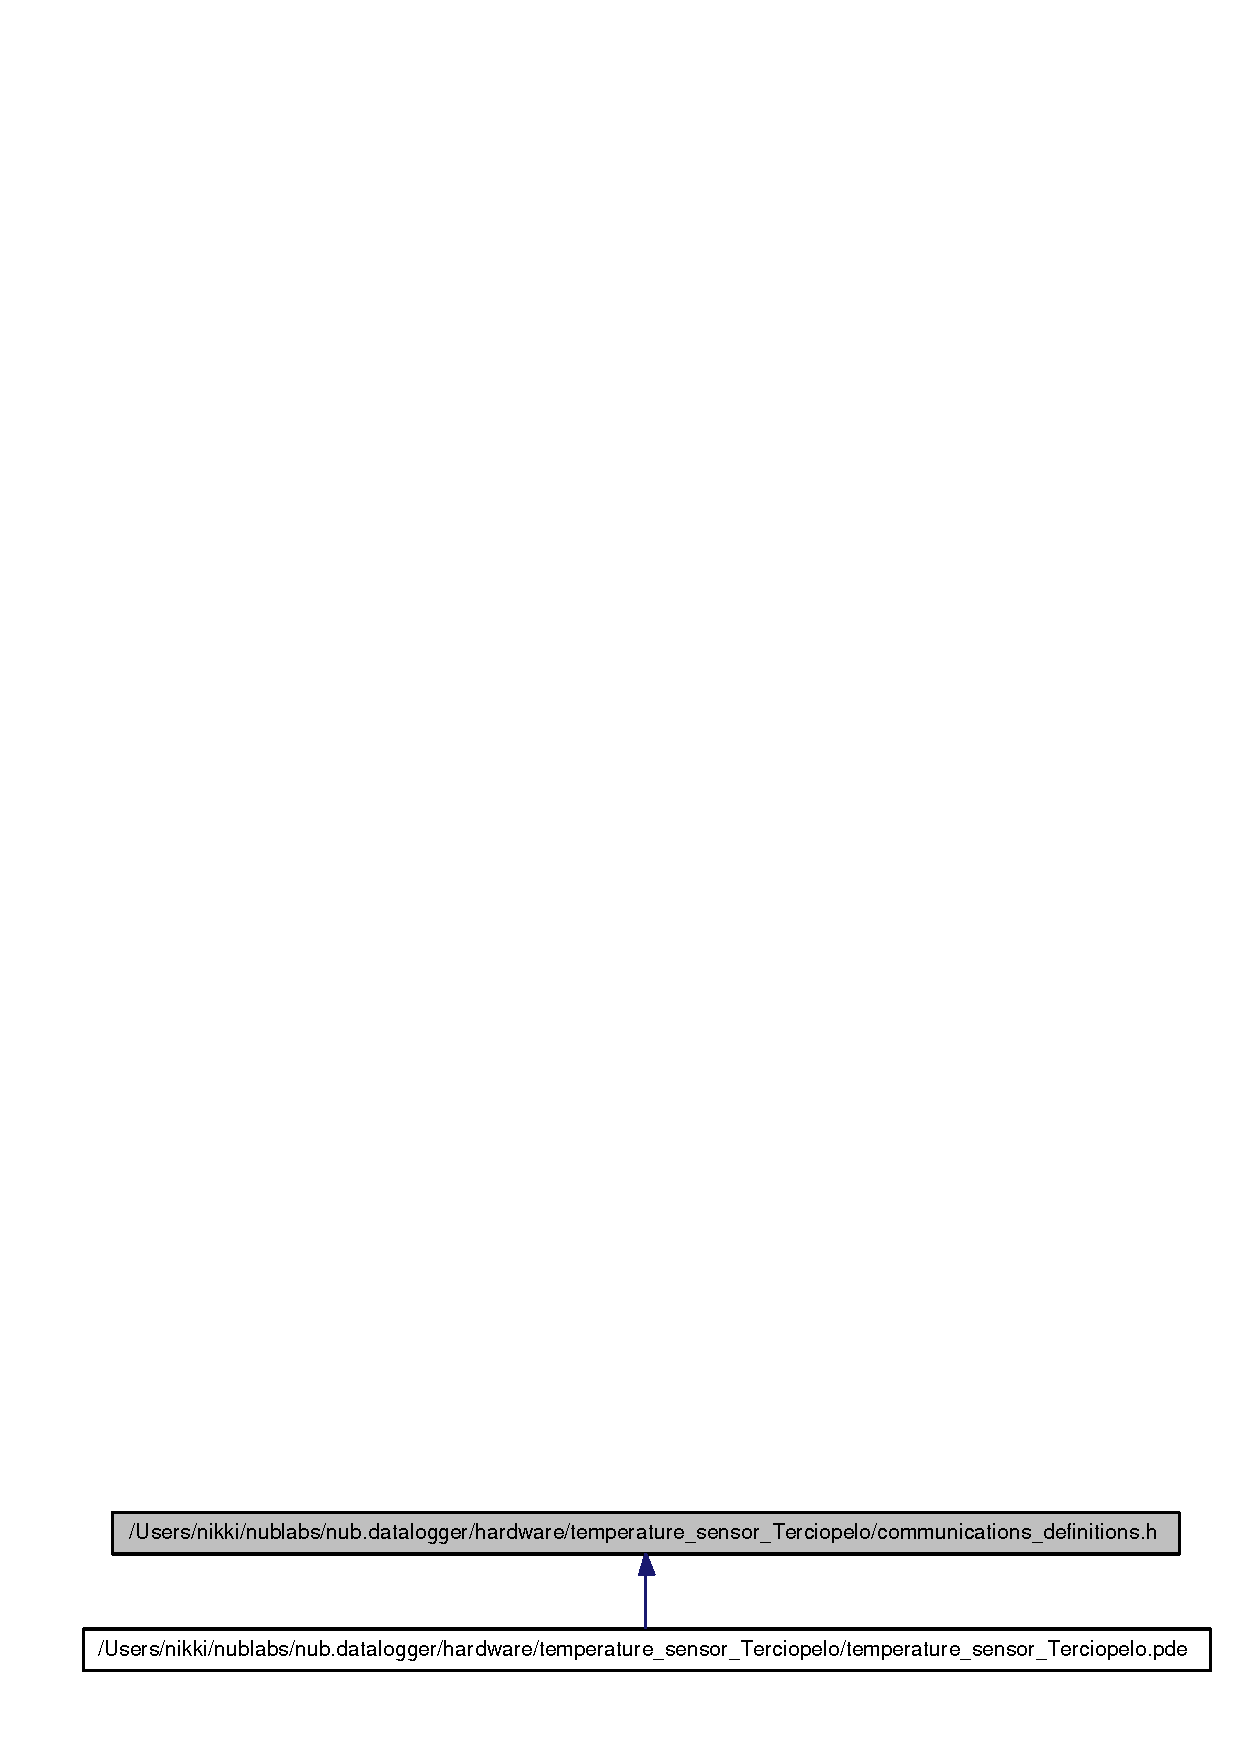
\includegraphics[width=292pt]{communications__definitions_8h__dep__incl}
\end{center}
\end{figure}
\subsection*{Defines}
\begin{CompactItemize}
\item 
\#define \hyperlink{communications__definitions_8h_1685ca2e434799fb98ea9272ed39d5e3}{NUM\_\-TRIES}~3
\item 
\#define \hyperlink{communications__definitions_8h_d97232eed56f4b8962167188db8dd2d4}{ACKNOWLEDGE}~1
\begin{CompactList}\small\item\em these are defined messages sent between the sensor and the computer \item\end{CompactList}\item 
\#define \hyperlink{communications__definitions_8h_421ea5726b2e7e3464457785964b3c11}{ACKNOWLEDGE\_\-AND\_\-CONFIGURE}~2
\item 
\#define \hyperlink{communications__definitions_8h_29d0028b064fb993c0e1f2b1ce4a7f88}{LISTENING}~3
\item 
\#define \hyperlink{communications__definitions_8h_d7285ac8b394b259876f0e61574dd8b0}{CHECKSUM\_\-ERROR\_\-PLEASE\_\-RESEND}~4
\item 
\#define \hyperlink{communications__definitions_8h_b111ad1c600abfe6a9a3a7e7a1a057d5}{CHECKSUM\_\-ERROR\_\-GIVING\_\-UP}~5
\item 
\#define \hyperlink{communications__definitions_8h_9413ad5afdb7d48c2d8606409cde00d0}{DISCOVER\_\-ME}~6
\item 
\#define \hyperlink{communications__definitions_8h_efc48d416c882f06edaf6d01779d4d74}{TIMEOUT\_\-ERROR}~7
\item 
\#define \hyperlink{communications__definitions_8h_c4da90313e5d11e20acac66663fb014c}{MALFORMED\_\-MESSAGE\_\-ERROR\_\-PLEASE\_\-RESEND}~8
\item 
\#define \hyperlink{communications__definitions_8h_bf39c03638711128272afb73031f864d}{MALFORMED\_\-MESSAGE\_\-ERROR\_\-GIVING\_\-UP}~9
\item 
\#define \hyperlink{communications__definitions_8h_53b51d504d04d1bbfb3d4a4f57349480}{MESSAGE\_\-START}~128
\item 
\#define \hyperlink{communications__definitions_8h_012714d5d0e7065e355fefe979491541}{MESSAGE\_\-END}~129
\item 
\#define \hyperlink{communications__definitions_8h_d82632844d46de002b8d8d16900e42a0}{HOUR\_\-HIGH}~1
\item 
\#define \hyperlink{communications__definitions_8h_3faa4fcb5d61433ccf65f19b4de44703}{HOUR\_\-LOW}~2
\item 
\#define \hyperlink{communications__definitions_8h_592fee6a2134a20e8761668cb7c773e3}{MINUTE\_\-HIGH}~3
\item 
\#define \hyperlink{communications__definitions_8h_2ace92e75321bdd463da760570b4e7e7}{MINUTE\_\-LOW}~4
\item 
\#define \hyperlink{communications__definitions_8h_f4364f097130bbbe71669acfee2692ae}{SECOND\_\-HIGH}~5
\item 
\#define \hyperlink{communications__definitions_8h_15e121356786cb610493f80e4b35e677}{SECOND\_\-LOW}~6
\item 
\#define \hyperlink{communications__definitions_8h_9886586c91a412164c69eb0270d2875e}{CHECKSUM}~7
\item 
\#define \hyperlink{communications__definitions_8h_8ec36de1ede672b53100e0414d57a75a}{CONFIGURATION\_\-MESSAGE\_\-LENGTH}~8
\end{CompactItemize}


\subsection{Define Documentation}
\hypertarget{communications__definitions_8h_d97232eed56f4b8962167188db8dd2d4}{
\index{communications\_\-definitions.h@{communications\_\-definitions.h}!ACKNOWLEDGE@{ACKNOWLEDGE}}
\index{ACKNOWLEDGE@{ACKNOWLEDGE}!communications_definitions.h@{communications\_\-definitions.h}}
\subsubsection[{ACKNOWLEDGE}]{\setlength{\rightskip}{0pt plus 5cm}\#define ACKNOWLEDGE~1}}
\label{communications__definitions_8h_d97232eed56f4b8962167188db8dd2d4}


these are defined messages sent between the sensor and the computer 



Definition at line 9 of file communications\_\-definitions.h.

Referenced by discover(), and sendData().\hypertarget{communications__definitions_8h_421ea5726b2e7e3464457785964b3c11}{
\index{communications\_\-definitions.h@{communications\_\-definitions.h}!ACKNOWLEDGE\_\-AND\_\-CONFIGURE@{ACKNOWLEDGE\_\-AND\_\-CONFIGURE}}
\index{ACKNOWLEDGE\_\-AND\_\-CONFIGURE@{ACKNOWLEDGE\_\-AND\_\-CONFIGURE}!communications_definitions.h@{communications\_\-definitions.h}}
\subsubsection[{ACKNOWLEDGE\_\-AND\_\-CONFIGURE}]{\setlength{\rightskip}{0pt plus 5cm}\#define ACKNOWLEDGE\_\-AND\_\-CONFIGURE~2}}
\label{communications__definitions_8h_421ea5726b2e7e3464457785964b3c11}




Definition at line 10 of file communications\_\-definitions.h.

Referenced by discover(), and sendData().\hypertarget{communications__definitions_8h_9886586c91a412164c69eb0270d2875e}{
\index{communications\_\-definitions.h@{communications\_\-definitions.h}!CHECKSUM@{CHECKSUM}}
\index{CHECKSUM@{CHECKSUM}!communications_definitions.h@{communications\_\-definitions.h}}
\subsubsection[{CHECKSUM}]{\setlength{\rightskip}{0pt plus 5cm}\#define CHECKSUM~7}}
\label{communications__definitions_8h_9886586c91a412164c69eb0270d2875e}




Definition at line 29 of file communications\_\-definitions.h.

Referenced by configure().\hypertarget{communications__definitions_8h_b111ad1c600abfe6a9a3a7e7a1a057d5}{
\index{communications\_\-definitions.h@{communications\_\-definitions.h}!CHECKSUM\_\-ERROR\_\-GIVING\_\-UP@{CHECKSUM\_\-ERROR\_\-GIVING\_\-UP}}
\index{CHECKSUM\_\-ERROR\_\-GIVING\_\-UP@{CHECKSUM\_\-ERROR\_\-GIVING\_\-UP}!communications_definitions.h@{communications\_\-definitions.h}}
\subsubsection[{CHECKSUM\_\-ERROR\_\-GIVING\_\-UP}]{\setlength{\rightskip}{0pt plus 5cm}\#define CHECKSUM\_\-ERROR\_\-GIVING\_\-UP~5}}
\label{communications__definitions_8h_b111ad1c600abfe6a9a3a7e7a1a057d5}




Definition at line 13 of file communications\_\-definitions.h.

Referenced by configure().\hypertarget{communications__definitions_8h_d7285ac8b394b259876f0e61574dd8b0}{
\index{communications\_\-definitions.h@{communications\_\-definitions.h}!CHECKSUM\_\-ERROR\_\-PLEASE\_\-RESEND@{CHECKSUM\_\-ERROR\_\-PLEASE\_\-RESEND}}
\index{CHECKSUM\_\-ERROR\_\-PLEASE\_\-RESEND@{CHECKSUM\_\-ERROR\_\-PLEASE\_\-RESEND}!communications_definitions.h@{communications\_\-definitions.h}}
\subsubsection[{CHECKSUM\_\-ERROR\_\-PLEASE\_\-RESEND}]{\setlength{\rightskip}{0pt plus 5cm}\#define CHECKSUM\_\-ERROR\_\-PLEASE\_\-RESEND~4}}
\label{communications__definitions_8h_d7285ac8b394b259876f0e61574dd8b0}




Definition at line 12 of file communications\_\-definitions.h.

Referenced by configure().\hypertarget{communications__definitions_8h_8ec36de1ede672b53100e0414d57a75a}{
\index{communications\_\-definitions.h@{communications\_\-definitions.h}!CONFIGURATION\_\-MESSAGE\_\-LENGTH@{CONFIGURATION\_\-MESSAGE\_\-LENGTH}}
\index{CONFIGURATION\_\-MESSAGE\_\-LENGTH@{CONFIGURATION\_\-MESSAGE\_\-LENGTH}!communications_definitions.h@{communications\_\-definitions.h}}
\subsubsection[{CONFIGURATION\_\-MESSAGE\_\-LENGTH}]{\setlength{\rightskip}{0pt plus 5cm}\#define CONFIGURATION\_\-MESSAGE\_\-LENGTH~8}}
\label{communications__definitions_8h_8ec36de1ede672b53100e0414d57a75a}




Definition at line 30 of file communications\_\-definitions.h.

Referenced by configure().\hypertarget{communications__definitions_8h_9413ad5afdb7d48c2d8606409cde00d0}{
\index{communications\_\-definitions.h@{communications\_\-definitions.h}!DISCOVER\_\-ME@{DISCOVER\_\-ME}}
\index{DISCOVER\_\-ME@{DISCOVER\_\-ME}!communications_definitions.h@{communications\_\-definitions.h}}
\subsubsection[{DISCOVER\_\-ME}]{\setlength{\rightskip}{0pt plus 5cm}\#define DISCOVER\_\-ME~6}}
\label{communications__definitions_8h_9413ad5afdb7d48c2d8606409cde00d0}




Definition at line 14 of file communications\_\-definitions.h.

Referenced by discover().\hypertarget{communications__definitions_8h_d82632844d46de002b8d8d16900e42a0}{
\index{communications\_\-definitions.h@{communications\_\-definitions.h}!HOUR\_\-HIGH@{HOUR\_\-HIGH}}
\index{HOUR\_\-HIGH@{HOUR\_\-HIGH}!communications_definitions.h@{communications\_\-definitions.h}}
\subsubsection[{HOUR\_\-HIGH}]{\setlength{\rightskip}{0pt plus 5cm}\#define HOUR\_\-HIGH~1}}
\label{communications__definitions_8h_d82632844d46de002b8d8d16900e42a0}




Definition at line 23 of file communications\_\-definitions.h.

Referenced by configure().\hypertarget{communications__definitions_8h_3faa4fcb5d61433ccf65f19b4de44703}{
\index{communications\_\-definitions.h@{communications\_\-definitions.h}!HOUR\_\-LOW@{HOUR\_\-LOW}}
\index{HOUR\_\-LOW@{HOUR\_\-LOW}!communications_definitions.h@{communications\_\-definitions.h}}
\subsubsection[{HOUR\_\-LOW}]{\setlength{\rightskip}{0pt plus 5cm}\#define HOUR\_\-LOW~2}}
\label{communications__definitions_8h_3faa4fcb5d61433ccf65f19b4de44703}




Definition at line 24 of file communications\_\-definitions.h.

Referenced by configure().\hypertarget{communications__definitions_8h_29d0028b064fb993c0e1f2b1ce4a7f88}{
\index{communications\_\-definitions.h@{communications\_\-definitions.h}!LISTENING@{LISTENING}}
\index{LISTENING@{LISTENING}!communications_definitions.h@{communications\_\-definitions.h}}
\subsubsection[{LISTENING}]{\setlength{\rightskip}{0pt plus 5cm}\#define LISTENING~3}}
\label{communications__definitions_8h_29d0028b064fb993c0e1f2b1ce4a7f88}




Definition at line 11 of file communications\_\-definitions.h.

Referenced by configure().\hypertarget{communications__definitions_8h_bf39c03638711128272afb73031f864d}{
\index{communications\_\-definitions.h@{communications\_\-definitions.h}!MALFORMED\_\-MESSAGE\_\-ERROR\_\-GIVING\_\-UP@{MALFORMED\_\-MESSAGE\_\-ERROR\_\-GIVING\_\-UP}}
\index{MALFORMED\_\-MESSAGE\_\-ERROR\_\-GIVING\_\-UP@{MALFORMED\_\-MESSAGE\_\-ERROR\_\-GIVING\_\-UP}!communications_definitions.h@{communications\_\-definitions.h}}
\subsubsection[{MALFORMED\_\-MESSAGE\_\-ERROR\_\-GIVING\_\-UP}]{\setlength{\rightskip}{0pt plus 5cm}\#define MALFORMED\_\-MESSAGE\_\-ERROR\_\-GIVING\_\-UP~9}}
\label{communications__definitions_8h_bf39c03638711128272afb73031f864d}




Definition at line 17 of file communications\_\-definitions.h.

Referenced by configure().\hypertarget{communications__definitions_8h_c4da90313e5d11e20acac66663fb014c}{
\index{communications\_\-definitions.h@{communications\_\-definitions.h}!MALFORMED\_\-MESSAGE\_\-ERROR\_\-PLEASE\_\-RESEND@{MALFORMED\_\-MESSAGE\_\-ERROR\_\-PLEASE\_\-RESEND}}
\index{MALFORMED\_\-MESSAGE\_\-ERROR\_\-PLEASE\_\-RESEND@{MALFORMED\_\-MESSAGE\_\-ERROR\_\-PLEASE\_\-RESEND}!communications_definitions.h@{communications\_\-definitions.h}}
\subsubsection[{MALFORMED\_\-MESSAGE\_\-ERROR\_\-PLEASE\_\-RESEND}]{\setlength{\rightskip}{0pt plus 5cm}\#define MALFORMED\_\-MESSAGE\_\-ERROR\_\-PLEASE\_\-RESEND~8}}
\label{communications__definitions_8h_c4da90313e5d11e20acac66663fb014c}




Definition at line 16 of file communications\_\-definitions.h.

Referenced by configure().\hypertarget{communications__definitions_8h_012714d5d0e7065e355fefe979491541}{
\index{communications\_\-definitions.h@{communications\_\-definitions.h}!MESSAGE\_\-END@{MESSAGE\_\-END}}
\index{MESSAGE\_\-END@{MESSAGE\_\-END}!communications_definitions.h@{communications\_\-definitions.h}}
\subsubsection[{MESSAGE\_\-END}]{\setlength{\rightskip}{0pt plus 5cm}\#define MESSAGE\_\-END~129}}
\label{communications__definitions_8h_012714d5d0e7065e355fefe979491541}




Definition at line 21 of file communications\_\-definitions.h.

Referenced by discover(), getMessage(), and sendData().\hypertarget{communications__definitions_8h_53b51d504d04d1bbfb3d4a4f57349480}{
\index{communications\_\-definitions.h@{communications\_\-definitions.h}!MESSAGE\_\-START@{MESSAGE\_\-START}}
\index{MESSAGE\_\-START@{MESSAGE\_\-START}!communications_definitions.h@{communications\_\-definitions.h}}
\subsubsection[{MESSAGE\_\-START}]{\setlength{\rightskip}{0pt plus 5cm}\#define MESSAGE\_\-START~128}}
\label{communications__definitions_8h_53b51d504d04d1bbfb3d4a4f57349480}




Definition at line 20 of file communications\_\-definitions.h.

Referenced by configure(), discover(), and sendData().\hypertarget{communications__definitions_8h_592fee6a2134a20e8761668cb7c773e3}{
\index{communications\_\-definitions.h@{communications\_\-definitions.h}!MINUTE\_\-HIGH@{MINUTE\_\-HIGH}}
\index{MINUTE\_\-HIGH@{MINUTE\_\-HIGH}!communications_definitions.h@{communications\_\-definitions.h}}
\subsubsection[{MINUTE\_\-HIGH}]{\setlength{\rightskip}{0pt plus 5cm}\#define MINUTE\_\-HIGH~3}}
\label{communications__definitions_8h_592fee6a2134a20e8761668cb7c773e3}




Definition at line 25 of file communications\_\-definitions.h.

Referenced by configure().\hypertarget{communications__definitions_8h_2ace92e75321bdd463da760570b4e7e7}{
\index{communications\_\-definitions.h@{communications\_\-definitions.h}!MINUTE\_\-LOW@{MINUTE\_\-LOW}}
\index{MINUTE\_\-LOW@{MINUTE\_\-LOW}!communications_definitions.h@{communications\_\-definitions.h}}
\subsubsection[{MINUTE\_\-LOW}]{\setlength{\rightskip}{0pt plus 5cm}\#define MINUTE\_\-LOW~4}}
\label{communications__definitions_8h_2ace92e75321bdd463da760570b4e7e7}




Definition at line 26 of file communications\_\-definitions.h.

Referenced by configure().\hypertarget{communications__definitions_8h_1685ca2e434799fb98ea9272ed39d5e3}{
\index{communications\_\-definitions.h@{communications\_\-definitions.h}!NUM\_\-TRIES@{NUM\_\-TRIES}}
\index{NUM\_\-TRIES@{NUM\_\-TRIES}!communications_definitions.h@{communications\_\-definitions.h}}
\subsubsection[{NUM\_\-TRIES}]{\setlength{\rightskip}{0pt plus 5cm}\#define NUM\_\-TRIES~3}}
\label{communications__definitions_8h_1685ca2e434799fb98ea9272ed39d5e3}


This file contains definitions for message bytes sent back and forth between the sensor and computer 

Definition at line 6 of file communications\_\-definitions.h.

Referenced by configure(), and sendData().\hypertarget{communications__definitions_8h_f4364f097130bbbe71669acfee2692ae}{
\index{communications\_\-definitions.h@{communications\_\-definitions.h}!SECOND\_\-HIGH@{SECOND\_\-HIGH}}
\index{SECOND\_\-HIGH@{SECOND\_\-HIGH}!communications_definitions.h@{communications\_\-definitions.h}}
\subsubsection[{SECOND\_\-HIGH}]{\setlength{\rightskip}{0pt plus 5cm}\#define SECOND\_\-HIGH~5}}
\label{communications__definitions_8h_f4364f097130bbbe71669acfee2692ae}




Definition at line 27 of file communications\_\-definitions.h.

Referenced by configure().\hypertarget{communications__definitions_8h_15e121356786cb610493f80e4b35e677}{
\index{communications\_\-definitions.h@{communications\_\-definitions.h}!SECOND\_\-LOW@{SECOND\_\-LOW}}
\index{SECOND\_\-LOW@{SECOND\_\-LOW}!communications_definitions.h@{communications\_\-definitions.h}}
\subsubsection[{SECOND\_\-LOW}]{\setlength{\rightskip}{0pt plus 5cm}\#define SECOND\_\-LOW~6}}
\label{communications__definitions_8h_15e121356786cb610493f80e4b35e677}




Definition at line 28 of file communications\_\-definitions.h.

Referenced by configure().\hypertarget{communications__definitions_8h_efc48d416c882f06edaf6d01779d4d74}{
\index{communications\_\-definitions.h@{communications\_\-definitions.h}!TIMEOUT\_\-ERROR@{TIMEOUT\_\-ERROR}}
\index{TIMEOUT\_\-ERROR@{TIMEOUT\_\-ERROR}!communications_definitions.h@{communications\_\-definitions.h}}
\subsubsection[{TIMEOUT\_\-ERROR}]{\setlength{\rightskip}{0pt plus 5cm}\#define TIMEOUT\_\-ERROR~7}}
\label{communications__definitions_8h_efc48d416c882f06edaf6d01779d4d74}




Definition at line 15 of file communications\_\-definitions.h.

Referenced by configure(), and discover().
\hypertarget{applet_2globals_8h}{
\section{/Users/nikki/nublabs/nub.datalogger/hardware/temperature\_\-sensor\_\-Terciopelo/applet/globals.h File Reference}
\label{applet_2globals_8h}\index{/Users/nikki/nublabs/nub.datalogger/hardware/temperature\_\-sensor\_\-Terciopelo/applet/globals.h@{/Users/nikki/nublabs/nub.datalogger/hardware/temperature\_\-sensor\_\-Terciopelo/applet/globals.h}}
}


This graph shows which files directly or indirectly include this file:\subsection*{Defines}
\begin{CompactItemize}
\item 
\#define \hyperlink{applet_2globals_8h_a93f0eb578d23995850d61f7d61c55c1}{FALSE}~0
\item 
\#define \hyperlink{applet_2globals_8h_a8cecfc5c5c054d2875c03e77b7be15d}{TRUE}~1
\end{CompactItemize}
\subsection*{Variables}
\begin{CompactItemize}
\item 
char \hyperlink{applet_2globals_8h_a0ec8ae62320ddf9e7b3d84d4cf01522}{message} \mbox{[}50\mbox{]}
\item 
char \hyperlink{applet_2globals_8h_514585400668872c199fe503d6259b83}{discovered} = TRUE
\item 
char \hyperlink{applet_2globals_8h_7bfacbf7b939bc01bfe63d7a2fdb0ad8}{configured} = TRUE
\item 
int \hyperlink{applet_2globals_8h_f23005df06fc3cd4264e5eee2dfa2f8c}{hours} = 0
\item 
int \hyperlink{applet_2globals_8h_b693b677bdc9ded12b06daf49778101c}{minutes} = 0
\item 
int \hyperlink{applet_2globals_8h_77bd4f876bdc3afed5acdd936f775d34}{seconds} = 0
\item 
int \hyperlink{applet_2globals_8h_b70b476584326d0e035cead4222998ee}{sampleNumber} = 0
\item 
char \hyperlink{applet_2globals_8h_d5e2d3a85512c52e869f6ad9a4c2808e}{buffer} \mbox{[}256\mbox{]}
\item 
unsigned char \hyperlink{applet_2globals_8h_5abc5420a7f15af7410173395b610ea8}{index} = 0
\item 
unsigned char \hyperlink{applet_2globals_8h_0558edb7889eddddb3a01e3956de01c4}{start} = 0
\item 
int \hyperlink{applet_2globals_8h_eb723e2da6dfcdda2972ff176b4aade2}{sensor1\_\-top}
\item 
int \hyperlink{applet_2globals_8h_c0cf7a4f555cb76b1b42a5ec73a1f582}{sensor1\_\-bottom}
\item 
int \hyperlink{applet_2globals_8h_53eeb261a3774d88f4d6528d7005d1f9}{sensor2\_\-top}
\item 
int \hyperlink{applet_2globals_8h_fa5a6e2e44e641853a69e229c54a8c6b}{sensor2\_\-bottom}
\item 
float \hyperlink{applet_2globals_8h_02e4140abf2d38e2f54630353cc82c4d}{sensor1\_\-resistance}
\item 
float \hyperlink{applet_2globals_8h_259f351e7df30a37af60b330915a2722}{sensor2\_\-resistance}
\item 
float \hyperlink{applet_2globals_8h_bffcded031596e15ce3964ab6ebe4f29}{sensor1\_\-temperature}
\item 
float \hyperlink{applet_2globals_8h_8e0d2769b71a81c3a75cc708611c00eb}{sensor2\_\-temperature}
\end{CompactItemize}


\subsection{Define Documentation}
\hypertarget{applet_2globals_8h_a93f0eb578d23995850d61f7d61c55c1}{
\index{applet/globals.h@{applet/globals.h}!FALSE@{FALSE}}
\index{FALSE@{FALSE}!applet/globals.h@{applet/globals.h}}
\subsubsection[{FALSE}]{\setlength{\rightskip}{0pt plus 5cm}\#define FALSE~0}}
\label{applet_2globals_8h_a93f0eb578d23995850d61f7d61c55c1}




Definition at line 1 of file globals.h.

Referenced by sendData().\hypertarget{applet_2globals_8h_a8cecfc5c5c054d2875c03e77b7be15d}{
\index{applet/globals.h@{applet/globals.h}!TRUE@{TRUE}}
\index{TRUE@{TRUE}!applet/globals.h@{applet/globals.h}}
\subsubsection[{TRUE}]{\setlength{\rightskip}{0pt plus 5cm}\#define TRUE~1}}
\label{applet_2globals_8h_a8cecfc5c5c054d2875c03e77b7be15d}




Definition at line 2 of file globals.h.

Referenced by discover(), and sendData().

\subsection{Variable Documentation}
\hypertarget{applet_2globals_8h_d5e2d3a85512c52e869f6ad9a4c2808e}{
\index{applet/globals.h@{applet/globals.h}!buffer@{buffer}}
\index{buffer@{buffer}!applet/globals.h@{applet/globals.h}}
\subsubsection[{buffer}]{\setlength{\rightskip}{0pt plus 5cm}char {\bf buffer}\mbox{[}256\mbox{]}}}
\label{applet_2globals_8h_d5e2d3a85512c52e869f6ad9a4c2808e}




Definition at line 20 of file globals.h.

Referenced by configure(), and getMessage().\hypertarget{applet_2globals_8h_7bfacbf7b939bc01bfe63d7a2fdb0ad8}{
\index{applet/globals.h@{applet/globals.h}!configured@{configured}}
\index{configured@{configured}!applet/globals.h@{applet/globals.h}}
\subsubsection[{configured}]{\setlength{\rightskip}{0pt plus 5cm}char {\bf configured} = TRUE}}
\label{applet_2globals_8h_7bfacbf7b939bc01bfe63d7a2fdb0ad8}




Definition at line 8 of file globals.h.

Referenced by configure().\hypertarget{applet_2globals_8h_514585400668872c199fe503d6259b83}{
\index{applet/globals.h@{applet/globals.h}!discovered@{discovered}}
\index{discovered@{discovered}!applet/globals.h@{applet/globals.h}}
\subsubsection[{discovered}]{\setlength{\rightskip}{0pt plus 5cm}char {\bf discovered} = TRUE}}
\label{applet_2globals_8h_514585400668872c199fe503d6259b83}




Definition at line 7 of file globals.h.

Referenced by discover().\hypertarget{applet_2globals_8h_f23005df06fc3cd4264e5eee2dfa2f8c}{
\index{applet/globals.h@{applet/globals.h}!hours@{hours}}
\index{hours@{hours}!applet/globals.h@{applet/globals.h}}
\subsubsection[{hours}]{\setlength{\rightskip}{0pt plus 5cm}int {\bf hours} = 0}}
\label{applet_2globals_8h_f23005df06fc3cd4264e5eee2dfa2f8c}




Definition at line 11 of file globals.h.

Referenced by configure().\hypertarget{applet_2globals_8h_5abc5420a7f15af7410173395b610ea8}{
\index{applet/globals.h@{applet/globals.h}!index@{index}}
\index{index@{index}!applet/globals.h@{applet/globals.h}}
\subsubsection[{index}]{\setlength{\rightskip}{0pt plus 5cm}unsigned char {\bf index} = 0}}
\label{applet_2globals_8h_5abc5420a7f15af7410173395b610ea8}




Definition at line 21 of file globals.h.

Referenced by configure(), and getMessage().\hypertarget{applet_2globals_8h_a0ec8ae62320ddf9e7b3d84d4cf01522}{
\index{applet/globals.h@{applet/globals.h}!message@{message}}
\index{message@{message}!applet/globals.h@{applet/globals.h}}
\subsubsection[{message}]{\setlength{\rightskip}{0pt plus 5cm}char {\bf message}\mbox{[}50\mbox{]}}}
\label{applet_2globals_8h_a0ec8ae62320ddf9e7b3d84d4cf01522}




Definition at line 5 of file globals.h.

Referenced by getChecksum(), and sendData().\hypertarget{applet_2globals_8h_b693b677bdc9ded12b06daf49778101c}{
\index{applet/globals.h@{applet/globals.h}!minutes@{minutes}}
\index{minutes@{minutes}!applet/globals.h@{applet/globals.h}}
\subsubsection[{minutes}]{\setlength{\rightskip}{0pt plus 5cm}int {\bf minutes} = 0}}
\label{applet_2globals_8h_b693b677bdc9ded12b06daf49778101c}




Definition at line 12 of file globals.h.

Referenced by configure(), and waitForSampleInterval().\hypertarget{applet_2globals_8h_b70b476584326d0e035cead4222998ee}{
\index{applet/globals.h@{applet/globals.h}!sampleNumber@{sampleNumber}}
\index{sampleNumber@{sampleNumber}!applet/globals.h@{applet/globals.h}}
\subsubsection[{sampleNumber}]{\setlength{\rightskip}{0pt plus 5cm}int {\bf sampleNumber} = 0}}
\label{applet_2globals_8h_b70b476584326d0e035cead4222998ee}




Definition at line 16 of file globals.h.

Referenced by sample(), and sendData().\hypertarget{applet_2globals_8h_77bd4f876bdc3afed5acdd936f775d34}{
\index{applet/globals.h@{applet/globals.h}!seconds@{seconds}}
\index{seconds@{seconds}!applet/globals.h@{applet/globals.h}}
\subsubsection[{seconds}]{\setlength{\rightskip}{0pt plus 5cm}int {\bf seconds} = 0}}
\label{applet_2globals_8h_77bd4f876bdc3afed5acdd936f775d34}




Definition at line 13 of file globals.h.

Referenced by configure(), and waitForSampleInterval().\hypertarget{applet_2globals_8h_c0cf7a4f555cb76b1b42a5ec73a1f582}{
\index{applet/globals.h@{applet/globals.h}!sensor1\_\-bottom@{sensor1\_\-bottom}}
\index{sensor1\_\-bottom@{sensor1\_\-bottom}!applet/globals.h@{applet/globals.h}}
\subsubsection[{sensor1\_\-bottom}]{\setlength{\rightskip}{0pt plus 5cm}int {\bf sensor1\_\-bottom}}}
\label{applet_2globals_8h_c0cf7a4f555cb76b1b42a5ec73a1f582}




Definition at line 26 of file globals.h.

Referenced by convertToResistance(), and getRawData().\hypertarget{applet_2globals_8h_02e4140abf2d38e2f54630353cc82c4d}{
\index{applet/globals.h@{applet/globals.h}!sensor1\_\-resistance@{sensor1\_\-resistance}}
\index{sensor1\_\-resistance@{sensor1\_\-resistance}!applet/globals.h@{applet/globals.h}}
\subsubsection[{sensor1\_\-resistance}]{\setlength{\rightskip}{0pt plus 5cm}float {\bf sensor1\_\-resistance}}}
\label{applet_2globals_8h_02e4140abf2d38e2f54630353cc82c4d}




Definition at line 31 of file globals.h.

Referenced by convertToResistance(), and convertToTemperature().\hypertarget{applet_2globals_8h_bffcded031596e15ce3964ab6ebe4f29}{
\index{applet/globals.h@{applet/globals.h}!sensor1\_\-temperature@{sensor1\_\-temperature}}
\index{sensor1\_\-temperature@{sensor1\_\-temperature}!applet/globals.h@{applet/globals.h}}
\subsubsection[{sensor1\_\-temperature}]{\setlength{\rightskip}{0pt plus 5cm}float {\bf sensor1\_\-temperature}}}
\label{applet_2globals_8h_bffcded031596e15ce3964ab6ebe4f29}




Definition at line 35 of file globals.h.

Referenced by convertToTemperature(), and sendData().\hypertarget{applet_2globals_8h_eb723e2da6dfcdda2972ff176b4aade2}{
\index{applet/globals.h@{applet/globals.h}!sensor1\_\-top@{sensor1\_\-top}}
\index{sensor1\_\-top@{sensor1\_\-top}!applet/globals.h@{applet/globals.h}}
\subsubsection[{sensor1\_\-top}]{\setlength{\rightskip}{0pt plus 5cm}int {\bf sensor1\_\-top}}}
\label{applet_2globals_8h_eb723e2da6dfcdda2972ff176b4aade2}




Definition at line 25 of file globals.h.

Referenced by convertToResistance(), and getRawData().\hypertarget{applet_2globals_8h_fa5a6e2e44e641853a69e229c54a8c6b}{
\index{applet/globals.h@{applet/globals.h}!sensor2\_\-bottom@{sensor2\_\-bottom}}
\index{sensor2\_\-bottom@{sensor2\_\-bottom}!applet/globals.h@{applet/globals.h}}
\subsubsection[{sensor2\_\-bottom}]{\setlength{\rightskip}{0pt plus 5cm}int {\bf sensor2\_\-bottom}}}
\label{applet_2globals_8h_fa5a6e2e44e641853a69e229c54a8c6b}




Definition at line 28 of file globals.h.\hypertarget{applet_2globals_8h_259f351e7df30a37af60b330915a2722}{
\index{applet/globals.h@{applet/globals.h}!sensor2\_\-resistance@{sensor2\_\-resistance}}
\index{sensor2\_\-resistance@{sensor2\_\-resistance}!applet/globals.h@{applet/globals.h}}
\subsubsection[{sensor2\_\-resistance}]{\setlength{\rightskip}{0pt plus 5cm}float {\bf sensor2\_\-resistance}}}
\label{applet_2globals_8h_259f351e7df30a37af60b330915a2722}




Definition at line 32 of file globals.h.\hypertarget{applet_2globals_8h_8e0d2769b71a81c3a75cc708611c00eb}{
\index{applet/globals.h@{applet/globals.h}!sensor2\_\-temperature@{sensor2\_\-temperature}}
\index{sensor2\_\-temperature@{sensor2\_\-temperature}!applet/globals.h@{applet/globals.h}}
\subsubsection[{sensor2\_\-temperature}]{\setlength{\rightskip}{0pt plus 5cm}float {\bf sensor2\_\-temperature}}}
\label{applet_2globals_8h_8e0d2769b71a81c3a75cc708611c00eb}




Definition at line 36 of file globals.h.\hypertarget{applet_2globals_8h_53eeb261a3774d88f4d6528d7005d1f9}{
\index{applet/globals.h@{applet/globals.h}!sensor2\_\-top@{sensor2\_\-top}}
\index{sensor2\_\-top@{sensor2\_\-top}!applet/globals.h@{applet/globals.h}}
\subsubsection[{sensor2\_\-top}]{\setlength{\rightskip}{0pt plus 5cm}int {\bf sensor2\_\-top}}}
\label{applet_2globals_8h_53eeb261a3774d88f4d6528d7005d1f9}




Definition at line 27 of file globals.h.\hypertarget{applet_2globals_8h_0558edb7889eddddb3a01e3956de01c4}{
\index{applet/globals.h@{applet/globals.h}!start@{start}}
\index{start@{start}!applet/globals.h@{applet/globals.h}}
\subsubsection[{start}]{\setlength{\rightskip}{0pt plus 5cm}unsigned char {\bf start} = 0}}
\label{applet_2globals_8h_0558edb7889eddddb3a01e3956de01c4}




Definition at line 22 of file globals.h.

Referenced by configure(), and getMessage().
\hypertarget{globals_8h}{
\section{/Users/nikki/nublabs/nub.datalogger/hardware/temperature\_\-sensor\_\-Terciopelo/globals.h File Reference}
\label{globals_8h}\index{/Users/nikki/nublabs/nub.datalogger/hardware/temperature\_\-sensor\_\-Terciopelo/globals.h@{/Users/nikki/nublabs/nub.datalogger/hardware/temperature\_\-sensor\_\-Terciopelo/globals.h}}
}


This graph shows which files directly or indirectly include this file:\nopagebreak
\begin{figure}[H]
\begin{center}
\leavevmode
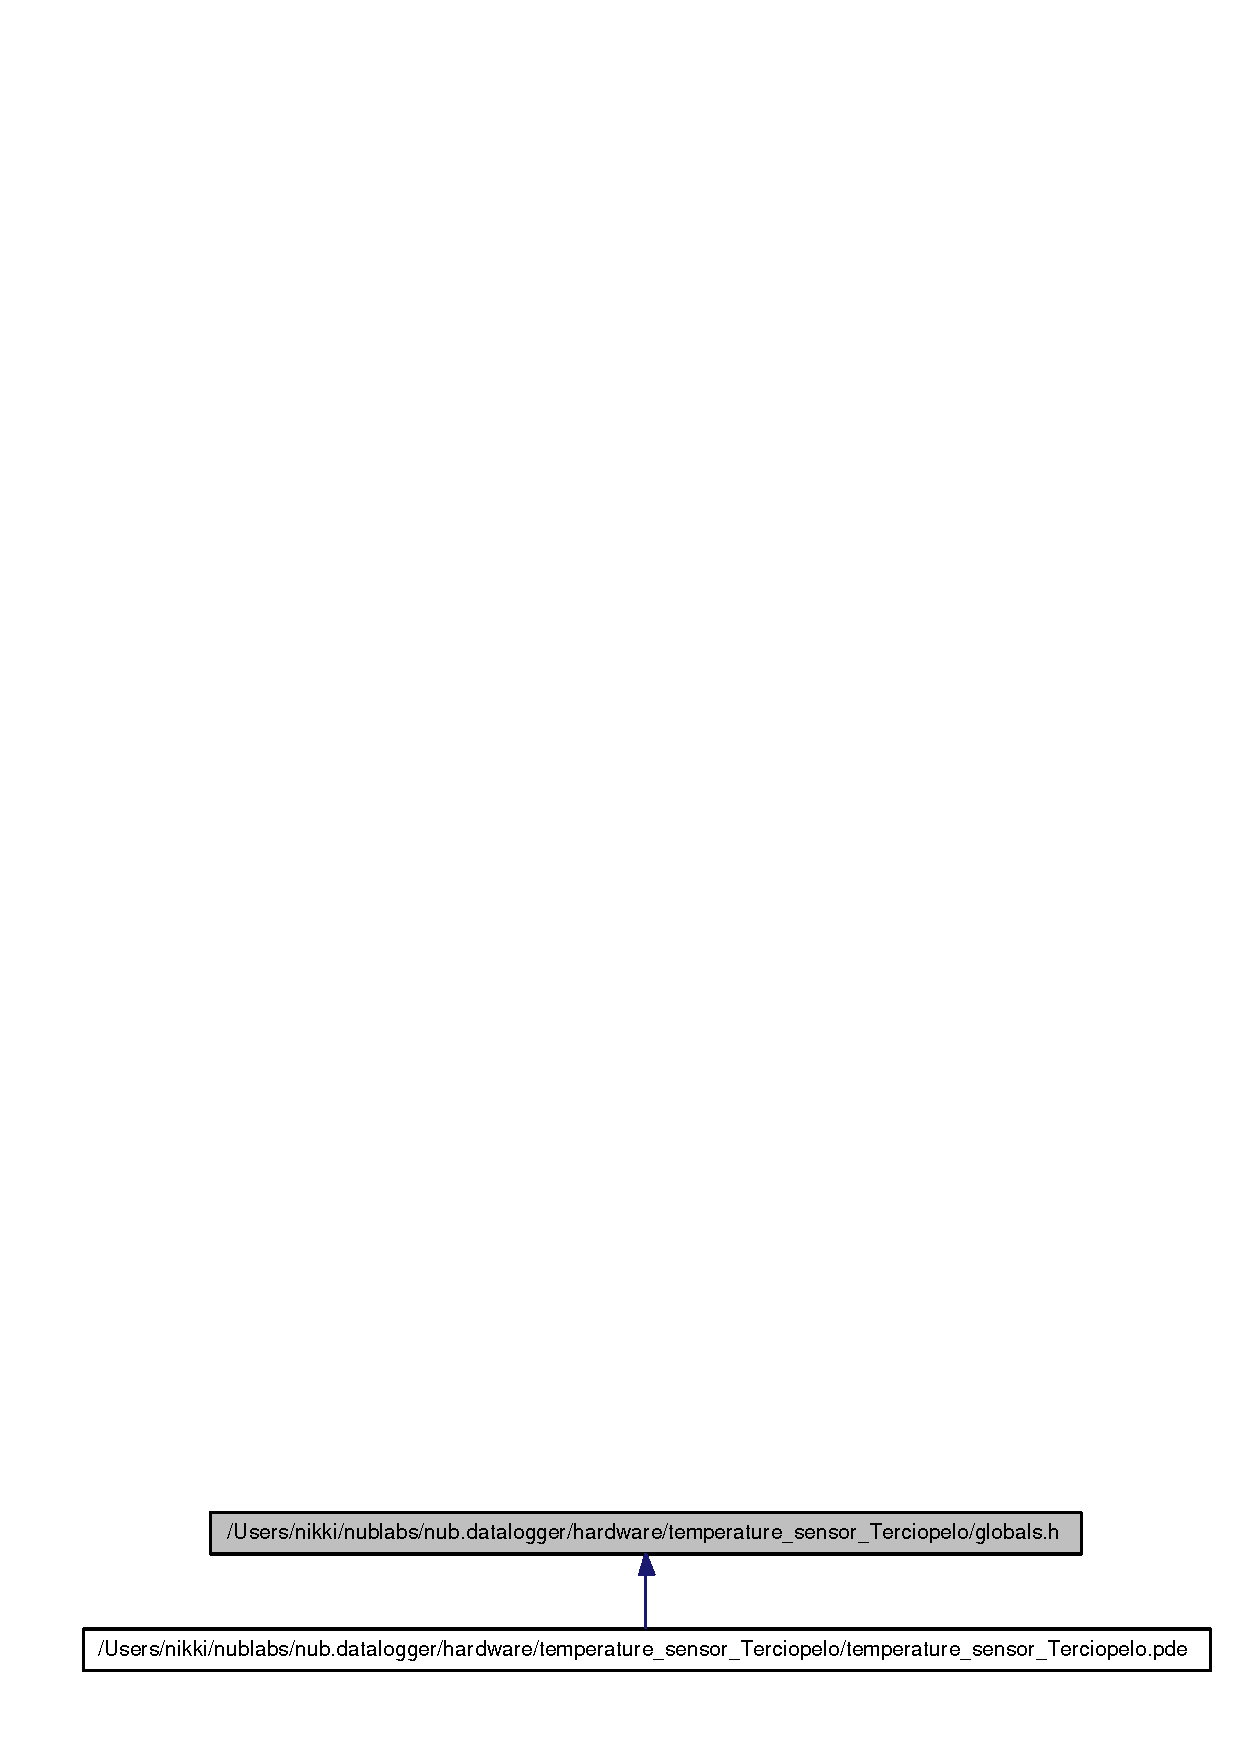
\includegraphics[width=292pt]{globals_8h__dep__incl}
\end{center}
\end{figure}
\subsection*{Defines}
\begin{CompactItemize}
\item 
\#define \hyperlink{globals_8h_a93f0eb578d23995850d61f7d61c55c1}{FALSE}~0
\item 
\#define \hyperlink{globals_8h_a8cecfc5c5c054d2875c03e77b7be15d}{TRUE}~1
\end{CompactItemize}
\subsection*{Variables}
\begin{CompactItemize}
\item 
char \hyperlink{globals_8h_a0ec8ae62320ddf9e7b3d84d4cf01522}{message} \mbox{[}50\mbox{]}
\item 
char \hyperlink{globals_8h_514585400668872c199fe503d6259b83}{discovered} = TRUE
\item 
char \hyperlink{globals_8h_7bfacbf7b939bc01bfe63d7a2fdb0ad8}{configured} = TRUE
\item 
int \hyperlink{globals_8h_f23005df06fc3cd4264e5eee2dfa2f8c}{hours} = 0
\item 
int \hyperlink{globals_8h_b693b677bdc9ded12b06daf49778101c}{minutes} = 0
\item 
int \hyperlink{globals_8h_77bd4f876bdc3afed5acdd936f775d34}{seconds} = 0
\item 
char \hyperlink{globals_8h_d5e2d3a85512c52e869f6ad9a4c2808e}{buffer} \mbox{[}256\mbox{]}
\item 
unsigned char \hyperlink{globals_8h_5abc5420a7f15af7410173395b610ea8}{index} = 0
\item 
unsigned char \hyperlink{globals_8h_0558edb7889eddddb3a01e3956de01c4}{start} = 0
\item 
int \hyperlink{globals_8h_eb723e2da6dfcdda2972ff176b4aade2}{sensor1\_\-top}
\item 
int \hyperlink{globals_8h_c0cf7a4f555cb76b1b42a5ec73a1f582}{sensor1\_\-bottom}
\item 
int \hyperlink{globals_8h_53eeb261a3774d88f4d6528d7005d1f9}{sensor2\_\-top}
\item 
int \hyperlink{globals_8h_fa5a6e2e44e641853a69e229c54a8c6b}{sensor2\_\-bottom}
\item 
float \hyperlink{globals_8h_02e4140abf2d38e2f54630353cc82c4d}{sensor1\_\-resistance}
\item 
float \hyperlink{globals_8h_259f351e7df30a37af60b330915a2722}{sensor2\_\-resistance}
\item 
float \hyperlink{globals_8h_bffcded031596e15ce3964ab6ebe4f29}{sensor1\_\-temperature}
\item 
float \hyperlink{globals_8h_8e0d2769b71a81c3a75cc708611c00eb}{sensor2\_\-temperature}
\end{CompactItemize}


\subsection{Define Documentation}
\hypertarget{globals_8h_a93f0eb578d23995850d61f7d61c55c1}{
\index{globals.h@{globals.h}!FALSE@{FALSE}}
\index{FALSE@{FALSE}!globals.h@{globals.h}}
\subsubsection[{FALSE}]{\setlength{\rightskip}{0pt plus 5cm}\#define FALSE~0}}
\label{globals_8h_a93f0eb578d23995850d61f7d61c55c1}




Definition at line 1 of file globals.h.

Referenced by sendData().\hypertarget{globals_8h_a8cecfc5c5c054d2875c03e77b7be15d}{
\index{globals.h@{globals.h}!TRUE@{TRUE}}
\index{TRUE@{TRUE}!globals.h@{globals.h}}
\subsubsection[{TRUE}]{\setlength{\rightskip}{0pt plus 5cm}\#define TRUE~1}}
\label{globals_8h_a8cecfc5c5c054d2875c03e77b7be15d}




Definition at line 2 of file globals.h.

Referenced by discover(), and sendData().

\subsection{Variable Documentation}
\hypertarget{globals_8h_d5e2d3a85512c52e869f6ad9a4c2808e}{
\index{globals.h@{globals.h}!buffer@{buffer}}
\index{buffer@{buffer}!globals.h@{globals.h}}
\subsubsection[{buffer}]{\setlength{\rightskip}{0pt plus 5cm}char {\bf buffer}\mbox{[}256\mbox{]}}}
\label{globals_8h_d5e2d3a85512c52e869f6ad9a4c2808e}




Definition at line 16 of file globals.h.

Referenced by configure(), and getMessage().\hypertarget{globals_8h_7bfacbf7b939bc01bfe63d7a2fdb0ad8}{
\index{globals.h@{globals.h}!configured@{configured}}
\index{configured@{configured}!globals.h@{globals.h}}
\subsubsection[{configured}]{\setlength{\rightskip}{0pt plus 5cm}char {\bf configured} = TRUE}}
\label{globals_8h_7bfacbf7b939bc01bfe63d7a2fdb0ad8}




Definition at line 8 of file globals.h.

Referenced by configure().\hypertarget{globals_8h_514585400668872c199fe503d6259b83}{
\index{globals.h@{globals.h}!discovered@{discovered}}
\index{discovered@{discovered}!globals.h@{globals.h}}
\subsubsection[{discovered}]{\setlength{\rightskip}{0pt plus 5cm}char {\bf discovered} = TRUE}}
\label{globals_8h_514585400668872c199fe503d6259b83}




Definition at line 7 of file globals.h.

Referenced by discover().\hypertarget{globals_8h_f23005df06fc3cd4264e5eee2dfa2f8c}{
\index{globals.h@{globals.h}!hours@{hours}}
\index{hours@{hours}!globals.h@{globals.h}}
\subsubsection[{hours}]{\setlength{\rightskip}{0pt plus 5cm}int {\bf hours} = 0}}
\label{globals_8h_f23005df06fc3cd4264e5eee2dfa2f8c}




Definition at line 11 of file globals.h.

Referenced by configure().\hypertarget{globals_8h_5abc5420a7f15af7410173395b610ea8}{
\index{globals.h@{globals.h}!index@{index}}
\index{index@{index}!globals.h@{globals.h}}
\subsubsection[{index}]{\setlength{\rightskip}{0pt plus 5cm}unsigned char {\bf index} = 0}}
\label{globals_8h_5abc5420a7f15af7410173395b610ea8}




Definition at line 17 of file globals.h.

Referenced by configure(), and getMessage().\hypertarget{globals_8h_a0ec8ae62320ddf9e7b3d84d4cf01522}{
\index{globals.h@{globals.h}!message@{message}}
\index{message@{message}!globals.h@{globals.h}}
\subsubsection[{message}]{\setlength{\rightskip}{0pt plus 5cm}char {\bf message}\mbox{[}50\mbox{]}}}
\label{globals_8h_a0ec8ae62320ddf9e7b3d84d4cf01522}




Definition at line 5 of file globals.h.

Referenced by getChecksum(), and sendData().\hypertarget{globals_8h_b693b677bdc9ded12b06daf49778101c}{
\index{globals.h@{globals.h}!minutes@{minutes}}
\index{minutes@{minutes}!globals.h@{globals.h}}
\subsubsection[{minutes}]{\setlength{\rightskip}{0pt plus 5cm}int {\bf minutes} = 0}}
\label{globals_8h_b693b677bdc9ded12b06daf49778101c}




Definition at line 12 of file globals.h.

Referenced by configure(), and waitForSampleInterval().\hypertarget{globals_8h_77bd4f876bdc3afed5acdd936f775d34}{
\index{globals.h@{globals.h}!seconds@{seconds}}
\index{seconds@{seconds}!globals.h@{globals.h}}
\subsubsection[{seconds}]{\setlength{\rightskip}{0pt plus 5cm}int {\bf seconds} = 0}}
\label{globals_8h_77bd4f876bdc3afed5acdd936f775d34}




Definition at line 13 of file globals.h.

Referenced by configure(), and waitForSampleInterval().\hypertarget{globals_8h_c0cf7a4f555cb76b1b42a5ec73a1f582}{
\index{globals.h@{globals.h}!sensor1\_\-bottom@{sensor1\_\-bottom}}
\index{sensor1\_\-bottom@{sensor1\_\-bottom}!globals.h@{globals.h}}
\subsubsection[{sensor1\_\-bottom}]{\setlength{\rightskip}{0pt plus 5cm}int {\bf sensor1\_\-bottom}}}
\label{globals_8h_c0cf7a4f555cb76b1b42a5ec73a1f582}




Definition at line 22 of file globals.h.

Referenced by convertToResistance(), and getRawData().\hypertarget{globals_8h_02e4140abf2d38e2f54630353cc82c4d}{
\index{globals.h@{globals.h}!sensor1\_\-resistance@{sensor1\_\-resistance}}
\index{sensor1\_\-resistance@{sensor1\_\-resistance}!globals.h@{globals.h}}
\subsubsection[{sensor1\_\-resistance}]{\setlength{\rightskip}{0pt plus 5cm}float {\bf sensor1\_\-resistance}}}
\label{globals_8h_02e4140abf2d38e2f54630353cc82c4d}




Definition at line 27 of file globals.h.

Referenced by convertToResistance(), and convertToTemperature().\hypertarget{globals_8h_bffcded031596e15ce3964ab6ebe4f29}{
\index{globals.h@{globals.h}!sensor1\_\-temperature@{sensor1\_\-temperature}}
\index{sensor1\_\-temperature@{sensor1\_\-temperature}!globals.h@{globals.h}}
\subsubsection[{sensor1\_\-temperature}]{\setlength{\rightskip}{0pt plus 5cm}float {\bf sensor1\_\-temperature}}}
\label{globals_8h_bffcded031596e15ce3964ab6ebe4f29}




Definition at line 31 of file globals.h.

Referenced by convertToTemperature(), and sendData().\hypertarget{globals_8h_eb723e2da6dfcdda2972ff176b4aade2}{
\index{globals.h@{globals.h}!sensor1\_\-top@{sensor1\_\-top}}
\index{sensor1\_\-top@{sensor1\_\-top}!globals.h@{globals.h}}
\subsubsection[{sensor1\_\-top}]{\setlength{\rightskip}{0pt plus 5cm}int {\bf sensor1\_\-top}}}
\label{globals_8h_eb723e2da6dfcdda2972ff176b4aade2}




Definition at line 21 of file globals.h.

Referenced by convertToResistance(), and getRawData().\hypertarget{globals_8h_fa5a6e2e44e641853a69e229c54a8c6b}{
\index{globals.h@{globals.h}!sensor2\_\-bottom@{sensor2\_\-bottom}}
\index{sensor2\_\-bottom@{sensor2\_\-bottom}!globals.h@{globals.h}}
\subsubsection[{sensor2\_\-bottom}]{\setlength{\rightskip}{0pt plus 5cm}int {\bf sensor2\_\-bottom}}}
\label{globals_8h_fa5a6e2e44e641853a69e229c54a8c6b}




Definition at line 24 of file globals.h.\hypertarget{globals_8h_259f351e7df30a37af60b330915a2722}{
\index{globals.h@{globals.h}!sensor2\_\-resistance@{sensor2\_\-resistance}}
\index{sensor2\_\-resistance@{sensor2\_\-resistance}!globals.h@{globals.h}}
\subsubsection[{sensor2\_\-resistance}]{\setlength{\rightskip}{0pt plus 5cm}float {\bf sensor2\_\-resistance}}}
\label{globals_8h_259f351e7df30a37af60b330915a2722}




Definition at line 28 of file globals.h.\hypertarget{globals_8h_8e0d2769b71a81c3a75cc708611c00eb}{
\index{globals.h@{globals.h}!sensor2\_\-temperature@{sensor2\_\-temperature}}
\index{sensor2\_\-temperature@{sensor2\_\-temperature}!globals.h@{globals.h}}
\subsubsection[{sensor2\_\-temperature}]{\setlength{\rightskip}{0pt plus 5cm}float {\bf sensor2\_\-temperature}}}
\label{globals_8h_8e0d2769b71a81c3a75cc708611c00eb}




Definition at line 32 of file globals.h.\hypertarget{globals_8h_53eeb261a3774d88f4d6528d7005d1f9}{
\index{globals.h@{globals.h}!sensor2\_\-top@{sensor2\_\-top}}
\index{sensor2\_\-top@{sensor2\_\-top}!globals.h@{globals.h}}
\subsubsection[{sensor2\_\-top}]{\setlength{\rightskip}{0pt plus 5cm}int {\bf sensor2\_\-top}}}
\label{globals_8h_53eeb261a3774d88f4d6528d7005d1f9}




Definition at line 23 of file globals.h.\hypertarget{globals_8h_0558edb7889eddddb3a01e3956de01c4}{
\index{globals.h@{globals.h}!start@{start}}
\index{start@{start}!globals.h@{globals.h}}
\subsubsection[{start}]{\setlength{\rightskip}{0pt plus 5cm}unsigned char {\bf start} = 0}}
\label{globals_8h_0558edb7889eddddb3a01e3956de01c4}




Definition at line 18 of file globals.h.

Referenced by configure(), and getMessage().
\hypertarget{applet_2name_8h}{
\section{/Users/nikki/nublabs/nub.datalogger/hardware/temperature\_\-sensor\_\-Terciopelo/applet/name.h File Reference}
\label{applet_2name_8h}\index{/Users/nikki/nublabs/nub.datalogger/hardware/temperature\_\-sensor\_\-Terciopelo/applet/name.h@{/Users/nikki/nublabs/nub.datalogger/hardware/temperature\_\-sensor\_\-Terciopelo/applet/name.h}}
}


This graph shows which files directly or indirectly include this file:\subsection*{Variables}
\begin{CompactItemize}
\item 
char $\ast$ \hyperlink{applet_2name_8h_5ac083a645d964373f022d03df4849c8}{name} = \char`\"{}albert\char`\"{}
\end{CompactItemize}


\subsection{Variable Documentation}
\hypertarget{applet_2name_8h_5ac083a645d964373f022d03df4849c8}{
\index{applet/name.h@{applet/name.h}!name@{name}}
\index{name@{name}!applet/name.h@{applet/name.h}}
\subsubsection[{name}]{\setlength{\rightskip}{0pt plus 5cm}char$\ast$ {\bf name} = \char`\"{}albert\char`\"{}}}
\label{applet_2name_8h_5ac083a645d964373f022d03df4849c8}




Definition at line 1 of file name.h.

Referenced by discover().
\hypertarget{name_8h}{
\section{/Users/nikki/nublabs/nub.datalogger/hardware/temperature\_\-sensor\_\-Terciopelo/name.h File Reference}
\label{name_8h}\index{/Users/nikki/nublabs/nub.datalogger/hardware/temperature\_\-sensor\_\-Terciopelo/name.h@{/Users/nikki/nublabs/nub.datalogger/hardware/temperature\_\-sensor\_\-Terciopelo/name.h}}
}


This graph shows which files directly or indirectly include this file:\subsection*{Variables}
\begin{CompactItemize}
\item 
char $\ast$ \hyperlink{name_8h_5ac083a645d964373f022d03df4849c8}{name} = \char`\"{}albert\char`\"{}
\end{CompactItemize}


\subsection{Variable Documentation}
\hypertarget{name_8h_5ac083a645d964373f022d03df4849c8}{
\index{name.h@{name.h}!name@{name}}
\index{name@{name}!name.h@{name.h}}
\subsubsection[{name}]{\setlength{\rightskip}{0pt plus 5cm}char$\ast$ {\bf name} = \char`\"{}albert\char`\"{}}}
\label{name_8h_5ac083a645d964373f022d03df4849c8}




Definition at line 1 of file name.h.

Referenced by discover().
\hypertarget{applet_2nublogger_8h}{
\section{/Users/nikki/nublabs/nub.datalogger/hardware/temperature\_\-sensor\_\-Terciopelo/applet/nublogger.h File Reference}
\label{applet_2nublogger_8h}\index{/Users/nikki/nublabs/nub.datalogger/hardware/temperature\_\-sensor\_\-Terciopelo/applet/nublogger.h@{/Users/nikki/nublabs/nub.datalogger/hardware/temperature\_\-sensor\_\-Terciopelo/applet/nublogger.h}}
}
{\tt \#include $<$HardwareSerial.h$>$}\par
{\tt \#include $<$string.h$>$}\par
{\tt \#include \char`\"{}communications.h\char`\"{}}\par


Include dependency graph for nublogger.h:\subsection*{Functions}
\begin{CompactItemize}
\item 
void \hyperlink{applet_2nublogger_8h_e369b3765489ee8bd0ea791c1843630f}{configure} ()
\begin{CompactList}\small\item\em \hyperlink{applet_2nublogger_8h_e369b3765489ee8bd0ea791c1843630f}{configure()} runs if the computer is trying to change the sensor's sample rate \item\end{CompactList}\item 
void \hyperlink{applet_2nublogger_8h_3fdb2350c3f98c0de0f0ae3c831a8b14}{discover} ()
\begin{CompactList}\small\item\em This function tells the computer of the datalogger's existence. \item\end{CompactList}\end{CompactItemize}


\subsection{Function Documentation}
\hypertarget{applet_2nublogger_8h_e369b3765489ee8bd0ea791c1843630f}{
\index{applet/nublogger.h@{applet/nublogger.h}!configure@{configure}}
\index{configure@{configure}!applet/nublogger.h@{applet/nublogger.h}}
\subsubsection[{configure}]{\setlength{\rightskip}{0pt plus 5cm}void configure ()}}
\label{applet_2nublogger_8h_e369b3765489ee8bd0ea791c1843630f}


\hyperlink{applet_2nublogger_8h_e369b3765489ee8bd0ea791c1843630f}{configure()} runs if the computer is trying to change the sensor's sample rate 

In \hyperlink{applet_2nublogger_8h_e369b3765489ee8bd0ea791c1843630f}{configure()}, the datalogger sends a LISTENING message to the computer, indicating that it's ready to receive data. The computer sends three ints: the hours, minutes and seconds of the sample interval, followed by a checksum byte that's the sum of the ints modulo 256. The sensor computes a checksum on the received data. If its checksum matches, it sends an ACKNOWLEDGE message back to the computer and updates its sample interval information. If the checksum does not match, it sends a CHECKSUM\_\-ERROR\_\-PLEASE\_\-RESEND message, asking the computer to send the three ints again, followed by a checksum. If the sensor can't get a valid message (with a matching checksum) after three tries, it gives up, sends a CHECKSUM\_\-ERROR\_\-GIVING\_\-UP message to the computer and keeps its original sample interval information

In \hyperlink{applet_2nublogger_8h_e369b3765489ee8bd0ea791c1843630f}{configure()}, the datalogger sends a LISTENING message to the computer, indicating that it's ready to receive data. The computer sends three ints: the hours, minutes and seconds of the sample interval, followed by a checksum byte that's the sum of the ints modulo 256. The sensor computes a checksum on the received data. If its checksum matches, it sends an ACKNOWLEDGE message back to the computer and updates its sample interval information. If the checksum does not match, it sends a CHECKSUM\_\-ERROR\_\-PLEASE\_\-RESEND message, asking the computer to send the three ints again, followed by a checksum. If the sensor can't get a valid message (with a matching checksum) after three tries, it gives up, sends a CHECKSUM\_\-ERROR\_\-GIVING\_\-UP message to the computer and keeps its original sample interval information 

Definition at line 15 of file nublogger.h.

Referenced by discover(), and sendData().

\begin{Code}\begin{verbatim}16 { 
17 }
\end{verbatim}
\end{Code}


\hypertarget{applet_2nublogger_8h_3fdb2350c3f98c0de0f0ae3c831a8b14}{
\index{applet/nublogger.h@{applet/nublogger.h}!discover@{discover}}
\index{discover@{discover}!applet/nublogger.h@{applet/nublogger.h}}
\subsubsection[{discover}]{\setlength{\rightskip}{0pt plus 5cm}void discover ()}}
\label{applet_2nublogger_8h_3fdb2350c3f98c0de0f0ae3c831a8b14}


This function tells the computer of the datalogger's existence. 

When the sensor turns on, it runs \hyperlink{applet_2nublogger_8h_3fdb2350c3f98c0de0f0ae3c831a8b14}{discover()}. It sends a MESSAGE\_\-START message, a DISCOVER\_\-ME message, and its name out to the computer and waits for acknowledgement. The computer can send back a plain \char`\"{}ACKNOWLEDGE\char`\"{} message, which means that the sensor should run using its default configuration values. The computer can also send back an \char`\"{}ACKNOWLEDGE\_\-AND\_\-CONFIGURE\char`\"{} message, which means that it has configuration data for the sensor. If the sensor gets this message, it'll run \hyperlink{applet_2nublogger_8h_e369b3765489ee8bd0ea791c1843630f}{configure()} to receive the data from the computer.

When the sensor turns on, it runs \hyperlink{applet_2nublogger_8h_3fdb2350c3f98c0de0f0ae3c831a8b14}{discover()}. It sends a MESSAGE\_\-START message, a DISCOVER\_\-ME message, and its name out to the computer and waits for acknowledgement. The computer can send back a plain \char`\"{}ACKNOWLEDGE\char`\"{} message, which means that the sensor should run using its default configuration values. The computer can also send back an \char`\"{}ACKNOWLEDGE\_\-AND\_\-CONFIGURE\char`\"{} message, which means that it has configuration data for the sensor. If the sensor gets this message, it'll run \hyperlink{applet_2nublogger_8h_e369b3765489ee8bd0ea791c1843630f}{configure()} to receive the data from the computer. 

Definition at line 27 of file nublogger.h.

Referenced by setup().

\begin{Code}\begin{verbatim}28 { 
29   unsigned char checksum=0;
30   int i=0;
31   Serial.print(MESSAGE_START, BYTE);
32   Serial.print(DISCOVER_ME,BYTE);
33   Serial.print(name);
34   while(name[i]!=0)
35   {
36     checksum+=name[i];
37     i++;
38   }
39   checksum+=DISCOVER_ME;
40   Serial.print(checksum,BYTE);
41   Serial.print(MESSAGE_END,BYTE);
42 
43   int receivedByte=getByte(100);     //looks for a byte on the serial port with a 100ms timeout
44   if(receivedByte==ACKNOWLEDGE)
45     discovered=TRUE;
46   if(receivedByte==ACKNOWLEDGE_AND_CONFIGURE)
47     {
48       discovered=TRUE;
49       configure();
50     }
51   
52 }
\end{verbatim}
\end{Code}



\hypertarget{nublogger_8h}{
\section{/Users/nikki/nublabs/nub.datalogger/hardware/temperature\_\-sensor\_\-Terciopelo/nublogger.h File Reference}
\label{nublogger_8h}\index{/Users/nikki/nublabs/nub.datalogger/hardware/temperature\_\-sensor\_\-Terciopelo/nublogger.h@{/Users/nikki/nublabs/nub.datalogger/hardware/temperature\_\-sensor\_\-Terciopelo/nublogger.h}}
}
{\tt \#include $<$HardwareSerial.h$>$}\par
{\tt \#include $<$string.h$>$}\par
{\tt \#include \char`\"{}communications.h\char`\"{}}\par


Include dependency graph for nublogger.h:\nopagebreak
\begin{figure}[H]
\begin{center}
\leavevmode
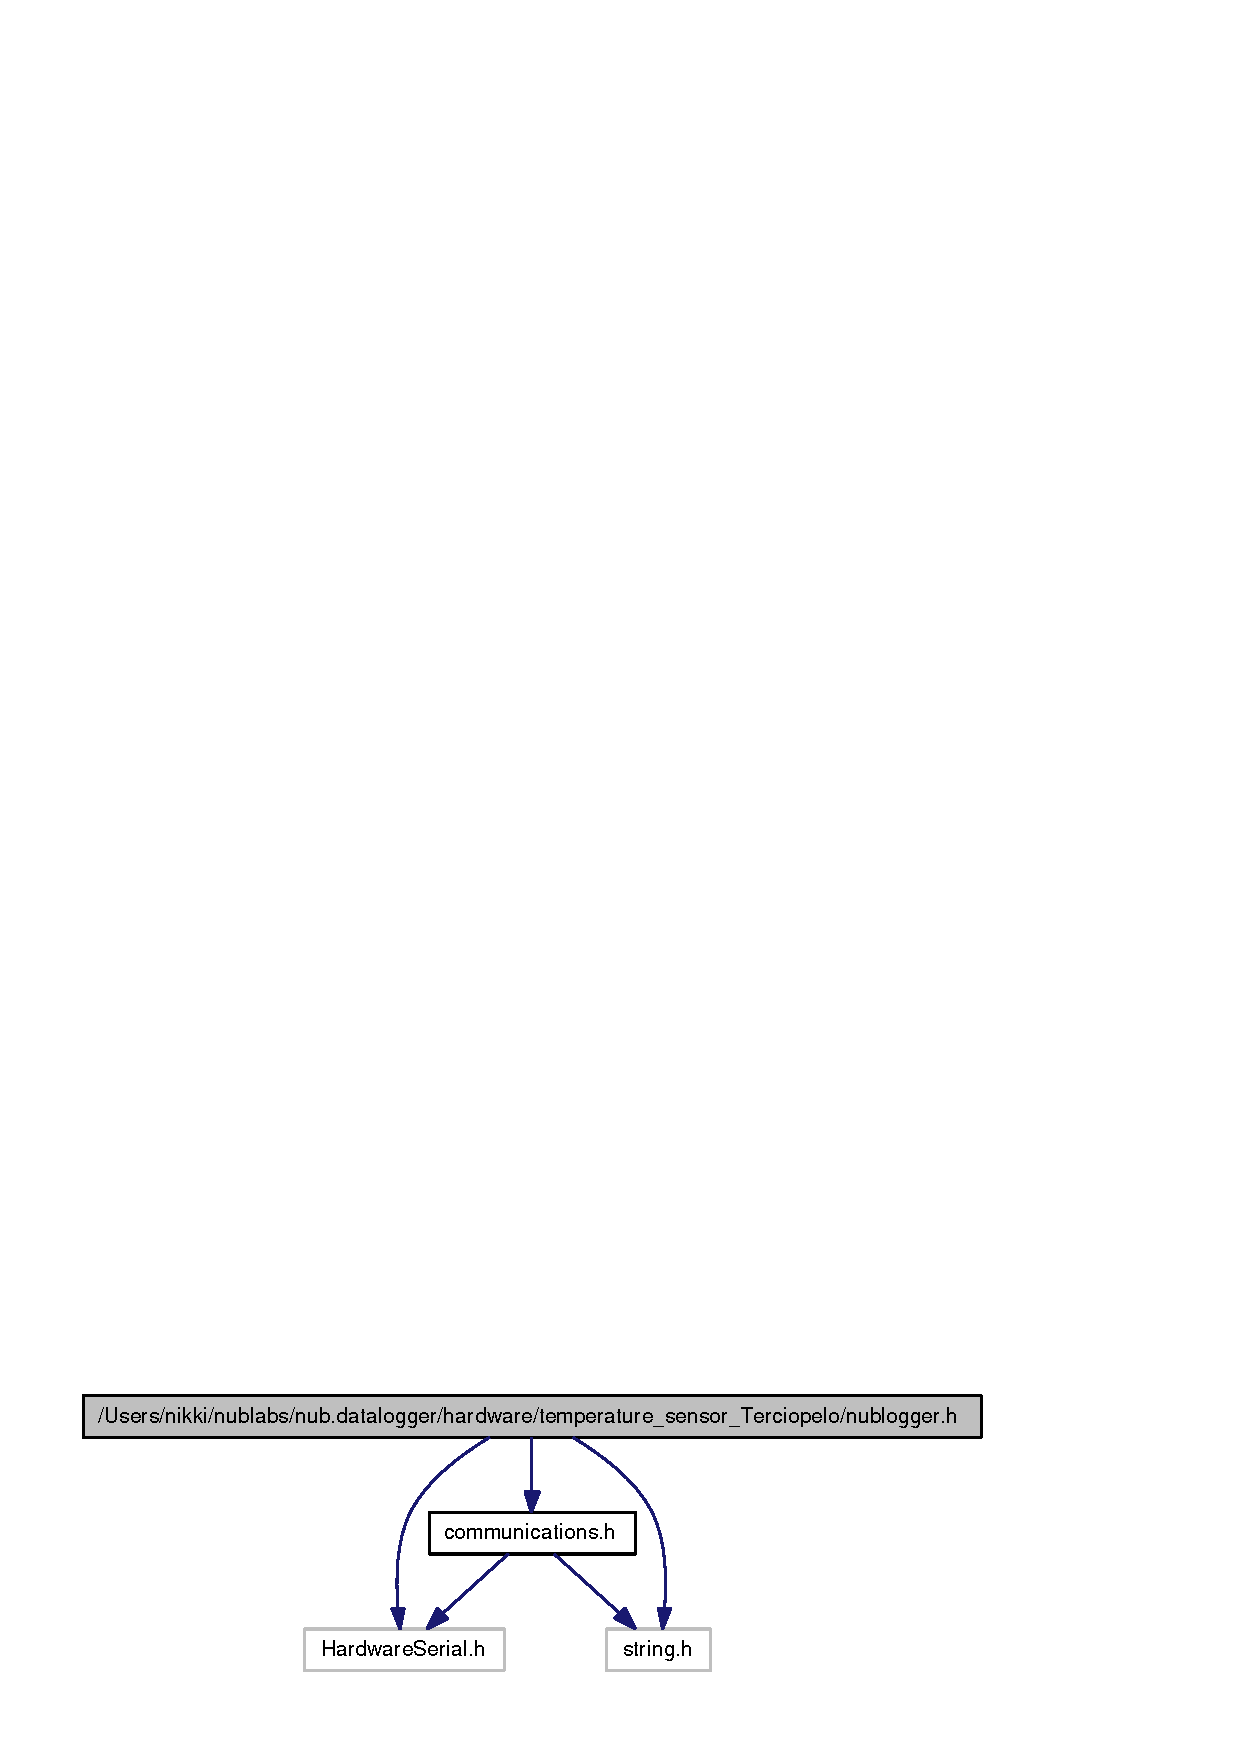
\includegraphics[width=237pt]{nublogger_8h__incl}
\end{center}
\end{figure}
\subsection*{Functions}
\begin{CompactItemize}
\item 
void \hyperlink{nublogger_8h_e369b3765489ee8bd0ea791c1843630f}{configure} ()
\begin{CompactList}\small\item\em \hyperlink{nublogger_8h_e369b3765489ee8bd0ea791c1843630f}{configure()} runs if the computer is trying to change the sensor's sample rate \item\end{CompactList}\item 
void \hyperlink{nublogger_8h_3fdb2350c3f98c0de0f0ae3c831a8b14}{discover} ()
\begin{CompactList}\small\item\em This function tells the computer of the datalogger's existence. \item\end{CompactList}\end{CompactItemize}


\subsection{Function Documentation}
\hypertarget{nublogger_8h_e369b3765489ee8bd0ea791c1843630f}{
\index{nublogger.h@{nublogger.h}!configure@{configure}}
\index{configure@{configure}!nublogger.h@{nublogger.h}}
\subsubsection[{configure}]{\setlength{\rightskip}{0pt plus 5cm}void configure ()}}
\label{nublogger_8h_e369b3765489ee8bd0ea791c1843630f}


\hyperlink{nublogger_8h_e369b3765489ee8bd0ea791c1843630f}{configure()} runs if the computer is trying to change the sensor's sample rate 

In \hyperlink{nublogger_8h_e369b3765489ee8bd0ea791c1843630f}{configure()}, the datalogger sends a LISTENING message to the computer, indicating that it's ready to receive data. The computer sends three ints: the hours, minutes and seconds of the sample interval, followed by a checksum byte that's the sum of the ints modulo 256. The sensor computes a checksum on the received data. If its checksum matches, it sends an ACKNOWLEDGE message back to the computer and updates its sample interval information. If the checksum does not match, it sends a CHECKSUM\_\-ERROR\_\-PLEASE\_\-RESEND message, asking the computer to send the three ints again, followed by a checksum. If the sensor can't get a valid message (with a matching checksum) after three tries, it gives up, sends a CHECKSUM\_\-ERROR\_\-GIVING\_\-UP message to the computer and keeps its original sample interval information 

Definition at line 15 of file nublogger.h.

Referenced by discover(), and sendData().

\begin{Code}\begin{verbatim}16 { 
17 }
\end{verbatim}
\end{Code}


\hypertarget{nublogger_8h_3fdb2350c3f98c0de0f0ae3c831a8b14}{
\index{nublogger.h@{nublogger.h}!discover@{discover}}
\index{discover@{discover}!nublogger.h@{nublogger.h}}
\subsubsection[{discover}]{\setlength{\rightskip}{0pt plus 5cm}void discover ()}}
\label{nublogger_8h_3fdb2350c3f98c0de0f0ae3c831a8b14}


This function tells the computer of the datalogger's existence. 

When the sensor turns on, it runs \hyperlink{nublogger_8h_3fdb2350c3f98c0de0f0ae3c831a8b14}{discover()}. It sends a MESSAGE\_\-START message, a DISCOVER\_\-ME message, and its name out to the computer and waits for acknowledgement. The computer can send back a plain \char`\"{}ACKNOWLEDGE\char`\"{} message, which means that the sensor should run using its default configuration values. The computer can also send back an \char`\"{}ACKNOWLEDGE\_\-AND\_\-CONFIGURE\char`\"{} message, which means that it has configuration data for the sensor. If the sensor gets this message, it'll run \hyperlink{nublogger_8h_e369b3765489ee8bd0ea791c1843630f}{configure()} to receive the data from the computer. 

Definition at line 27 of file nublogger.h.

References ACKNOWLEDGE, ACKNOWLEDGE\_\-AND\_\-CONFIGURE, configure(), DISCOVER\_\-ME, discovered, getByte(), MESSAGE\_\-END, MESSAGE\_\-START, name, and TRUE.

Referenced by setup().

\begin{Code}\begin{verbatim}28 { 
29   unsigned char checksum=0;
30   int i=0;
31   Serial.print(MESSAGE_START, BYTE);
32   Serial.print(DISCOVER_ME,BYTE);
33   Serial.print(name);
34   while(name[i]!=0)
35   {
36     checksum+=name[i];
37     i++;
38   }
39   checksum+=DISCOVER_ME;
40   Serial.print(checksum,BYTE);
41   Serial.print(MESSAGE_END,BYTE);
42 
43   int receivedByte=getByte(100);     //looks for a byte on the serial port with a 100ms timeout
44   if(receivedByte==ACKNOWLEDGE)
45     discovered=TRUE;
46   if(receivedByte==ACKNOWLEDGE_AND_CONFIGURE)
47     {
48       discovered=TRUE;
49       configure();
50     }
51   
52 }
\end{verbatim}
\end{Code}



\hypertarget{applet_2temperature__sensor__board__v2_8h}{
\section{/Users/nikki/nublabs/nub.datalogger/hardware/temperature\_\-sensor\_\-Terciopelo/applet/temperature\_\-sensor\_\-board\_\-v2.h File Reference}
\label{applet_2temperature__sensor__board__v2_8h}\index{/Users/nikki/nublabs/nub.datalogger/hardware/temperature\_\-sensor\_\-Terciopelo/applet/temperature\_\-sensor\_\-board\_\-v2.h@{/Users/nikki/nublabs/nub.datalogger/hardware/temperature\_\-sensor\_\-Terciopelo/applet/temperature\_\-sensor\_\-board\_\-v2.h}}
}
\subsection*{Defines}
\begin{CompactItemize}
\item 
\#define \hyperlink{applet_2temperature__sensor__board__v2_8h_658c2878485cfe5cc625d283a6d34bc1}{XBEE\_\-SLEEP}~2
\item 
\#define \hyperlink{applet_2temperature__sensor__board__v2_8h_b2de299215608c2a35f0feb86adc2f6f}{SAMPLE\_\-BUTTON}~3
\item 
\#define \hyperlink{applet_2temperature__sensor__board__v2_8h_eb7a7ba1ab7e0406f1b5ab36d579f585}{LED}~4
\item 
\#define \hyperlink{applet_2temperature__sensor__board__v2_8h_2a2946288d28852ba343b09fd4f17d7a}{SENSOR1\_\-TOP}~0
\item 
\#define \hyperlink{applet_2temperature__sensor__board__v2_8h_0da2a51dcb3e00b10aedd07d75f22382}{SENSOR1\_\-BOTTOM}~1
\item 
\#define \hyperlink{applet_2temperature__sensor__board__v2_8h_645141ae2ab7fa7ac3f690c4959b6baf}{SENSOR2\_\-TOP}~2
\item 
\#define \hyperlink{applet_2temperature__sensor__board__v2_8h_df66e6da6cf8c78004dc0a75fd14d3b1}{SENSOR2\_\-BOTTOM}~3
\end{CompactItemize}
\subsection*{Functions}
\begin{CompactItemize}
\item 
void \hyperlink{applet_2temperature__sensor__board__v2_8h_f6c9587ccbcf223f8c79f508c2fef366}{initializeSensor} ()
\begin{CompactList}\small\item\em this function configures all the digital communication pins as input or output pins \item\end{CompactList}\end{CompactItemize}


\subsection{Define Documentation}
\hypertarget{applet_2temperature__sensor__board__v2_8h_eb7a7ba1ab7e0406f1b5ab36d579f585}{
\index{applet/temperature\_\-sensor\_\-board\_\-v2.h@{applet/temperature\_\-sensor\_\-board\_\-v2.h}!LED@{LED}}
\index{LED@{LED}!applet/temperature_sensor_board_v2.h@{applet/temperature\_\-sensor\_\-board\_\-v2.h}}
\subsubsection[{LED}]{\setlength{\rightskip}{0pt plus 5cm}\#define LED~4}}
\label{applet_2temperature__sensor__board__v2_8h_eb7a7ba1ab7e0406f1b5ab36d579f585}




Definition at line 21 of file temperature\_\-sensor\_\-board\_\-v2.h.

Referenced by initializeSensor().\hypertarget{applet_2temperature__sensor__board__v2_8h_b2de299215608c2a35f0feb86adc2f6f}{
\index{applet/temperature\_\-sensor\_\-board\_\-v2.h@{applet/temperature\_\-sensor\_\-board\_\-v2.h}!SAMPLE\_\-BUTTON@{SAMPLE\_\-BUTTON}}
\index{SAMPLE\_\-BUTTON@{SAMPLE\_\-BUTTON}!applet/temperature_sensor_board_v2.h@{applet/temperature\_\-sensor\_\-board\_\-v2.h}}
\subsubsection[{SAMPLE\_\-BUTTON}]{\setlength{\rightskip}{0pt plus 5cm}\#define SAMPLE\_\-BUTTON~3}}
\label{applet_2temperature__sensor__board__v2_8h_b2de299215608c2a35f0feb86adc2f6f}




Definition at line 20 of file temperature\_\-sensor\_\-board\_\-v2.h.

Referenced by initializeSensor().\hypertarget{applet_2temperature__sensor__board__v2_8h_0da2a51dcb3e00b10aedd07d75f22382}{
\index{applet/temperature\_\-sensor\_\-board\_\-v2.h@{applet/temperature\_\-sensor\_\-board\_\-v2.h}!SENSOR1\_\-BOTTOM@{SENSOR1\_\-BOTTOM}}
\index{SENSOR1\_\-BOTTOM@{SENSOR1\_\-BOTTOM}!applet/temperature_sensor_board_v2.h@{applet/temperature\_\-sensor\_\-board\_\-v2.h}}
\subsubsection[{SENSOR1\_\-BOTTOM}]{\setlength{\rightskip}{0pt plus 5cm}\#define SENSOR1\_\-BOTTOM~1}}
\label{applet_2temperature__sensor__board__v2_8h_0da2a51dcb3e00b10aedd07d75f22382}




Definition at line 24 of file temperature\_\-sensor\_\-board\_\-v2.h.\hypertarget{applet_2temperature__sensor__board__v2_8h_2a2946288d28852ba343b09fd4f17d7a}{
\index{applet/temperature\_\-sensor\_\-board\_\-v2.h@{applet/temperature\_\-sensor\_\-board\_\-v2.h}!SENSOR1\_\-TOP@{SENSOR1\_\-TOP}}
\index{SENSOR1\_\-TOP@{SENSOR1\_\-TOP}!applet/temperature_sensor_board_v2.h@{applet/temperature\_\-sensor\_\-board\_\-v2.h}}
\subsubsection[{SENSOR1\_\-TOP}]{\setlength{\rightskip}{0pt plus 5cm}\#define SENSOR1\_\-TOP~0}}
\label{applet_2temperature__sensor__board__v2_8h_2a2946288d28852ba343b09fd4f17d7a}




Definition at line 23 of file temperature\_\-sensor\_\-board\_\-v2.h.\hypertarget{applet_2temperature__sensor__board__v2_8h_df66e6da6cf8c78004dc0a75fd14d3b1}{
\index{applet/temperature\_\-sensor\_\-board\_\-v2.h@{applet/temperature\_\-sensor\_\-board\_\-v2.h}!SENSOR2\_\-BOTTOM@{SENSOR2\_\-BOTTOM}}
\index{SENSOR2\_\-BOTTOM@{SENSOR2\_\-BOTTOM}!applet/temperature_sensor_board_v2.h@{applet/temperature\_\-sensor\_\-board\_\-v2.h}}
\subsubsection[{SENSOR2\_\-BOTTOM}]{\setlength{\rightskip}{0pt plus 5cm}\#define SENSOR2\_\-BOTTOM~3}}
\label{applet_2temperature__sensor__board__v2_8h_df66e6da6cf8c78004dc0a75fd14d3b1}




Definition at line 26 of file temperature\_\-sensor\_\-board\_\-v2.h.\hypertarget{applet_2temperature__sensor__board__v2_8h_645141ae2ab7fa7ac3f690c4959b6baf}{
\index{applet/temperature\_\-sensor\_\-board\_\-v2.h@{applet/temperature\_\-sensor\_\-board\_\-v2.h}!SENSOR2\_\-TOP@{SENSOR2\_\-TOP}}
\index{SENSOR2\_\-TOP@{SENSOR2\_\-TOP}!applet/temperature_sensor_board_v2.h@{applet/temperature\_\-sensor\_\-board\_\-v2.h}}
\subsubsection[{SENSOR2\_\-TOP}]{\setlength{\rightskip}{0pt plus 5cm}\#define SENSOR2\_\-TOP~2}}
\label{applet_2temperature__sensor__board__v2_8h_645141ae2ab7fa7ac3f690c4959b6baf}




Definition at line 25 of file temperature\_\-sensor\_\-board\_\-v2.h.\hypertarget{applet_2temperature__sensor__board__v2_8h_658c2878485cfe5cc625d283a6d34bc1}{
\index{applet/temperature\_\-sensor\_\-board\_\-v2.h@{applet/temperature\_\-sensor\_\-board\_\-v2.h}!XBEE\_\-SLEEP@{XBEE\_\-SLEEP}}
\index{XBEE\_\-SLEEP@{XBEE\_\-SLEEP}!applet/temperature_sensor_board_v2.h@{applet/temperature\_\-sensor\_\-board\_\-v2.h}}
\subsubsection[{XBEE\_\-SLEEP}]{\setlength{\rightskip}{0pt plus 5cm}\#define XBEE\_\-SLEEP~2}}
\label{applet_2temperature__sensor__board__v2_8h_658c2878485cfe5cc625d283a6d34bc1}


these are the pin definitions for the v2 board

function atmega pin arduino pin

Serial RX PD0 0 //serial lines that go out to the xbee module Serial TX PD1 1 Xbee\_\-sleep PD2 2 //a pin that, when asserted, puts the xbee radio into a low power sleep mode Sample\_\-button PD3 3 //an optional button that forces the sensor to take and send out a measurement LED PD4 4 //an LED on board that you can use for all kinds of stuff

sensor1\_\-top PC0 (analog) 0 sensor1\_\-bottom PC1 (analog) 1 sensor2\_\-top PC2 (analog) 2 sensor2\_\-bottom PC3 (analog) 3 

Definition at line 19 of file temperature\_\-sensor\_\-board\_\-v2.h.

Referenced by initializeSensor(), xbeeSleep(), and xbeeWake().

\subsection{Function Documentation}
\hypertarget{applet_2temperature__sensor__board__v2_8h_f6c9587ccbcf223f8c79f508c2fef366}{
\index{applet/temperature\_\-sensor\_\-board\_\-v2.h@{applet/temperature\_\-sensor\_\-board\_\-v2.h}!initializeSensor@{initializeSensor}}
\index{initializeSensor@{initializeSensor}!applet/temperature_sensor_board_v2.h@{applet/temperature\_\-sensor\_\-board\_\-v2.h}}
\subsubsection[{initializeSensor}]{\setlength{\rightskip}{0pt plus 5cm}void initializeSensor ()}}
\label{applet_2temperature__sensor__board__v2_8h_f6c9587ccbcf223f8c79f508c2fef366}


this function configures all the digital communication pins as input or output pins 

If you adapt this code to work with another sensor or board, you should replace the code in \hyperlink{applet_2temperature__sensor__board__v2_8h_f6c9587ccbcf223f8c79f508c2fef366}{initializeSensor()} to initialize all your relevant pins

If you adapt this code to work with another sensor or board, you should replace the code in \hyperlink{applet_2temperature__sensor__board__v2_8h_f6c9587ccbcf223f8c79f508c2fef366}{initializeSensor()} to initialize all your relevant pins 

Definition at line 35 of file temperature\_\-sensor\_\-board\_\-v2.h.

Referenced by setup().

\begin{Code}\begin{verbatim}36  {
37    pinMode(XBEE_SLEEP,OUTPUT);
38    pinMode(SAMPLE_BUTTON,INPUT);
39    pinMode(LED,OUTPUT);
40  }
\end{verbatim}
\end{Code}



\hypertarget{temperature__sensor__board__v2_8h}{
\section{/Users/nikki/nublabs/nub.datalogger/hardware/temperature\_\-sensor\_\-Terciopelo/temperature\_\-sensor\_\-board\_\-v2.h File Reference}
\label{temperature__sensor__board__v2_8h}\index{/Users/nikki/nublabs/nub.datalogger/hardware/temperature\_\-sensor\_\-Terciopelo/temperature\_\-sensor\_\-board\_\-v2.h@{/Users/nikki/nublabs/nub.datalogger/hardware/temperature\_\-sensor\_\-Terciopelo/temperature\_\-sensor\_\-board\_\-v2.h}}
}


This graph shows which files directly or indirectly include this file:\subsection*{Defines}
\begin{CompactItemize}
\item 
\#define \hyperlink{temperature__sensor__board__v2_8h_658c2878485cfe5cc625d283a6d34bc1}{XBEE\_\-SLEEP}~2
\item 
\#define \hyperlink{temperature__sensor__board__v2_8h_b2de299215608c2a35f0feb86adc2f6f}{SAMPLE\_\-BUTTON}~3
\item 
\#define \hyperlink{temperature__sensor__board__v2_8h_eb7a7ba1ab7e0406f1b5ab36d579f585}{LED}~4
\item 
\#define \hyperlink{temperature__sensor__board__v2_8h_2a2946288d28852ba343b09fd4f17d7a}{SENSOR1\_\-TOP}~0
\item 
\#define \hyperlink{temperature__sensor__board__v2_8h_0da2a51dcb3e00b10aedd07d75f22382}{SENSOR1\_\-BOTTOM}~1
\item 
\#define \hyperlink{temperature__sensor__board__v2_8h_645141ae2ab7fa7ac3f690c4959b6baf}{SENSOR2\_\-TOP}~2
\item 
\#define \hyperlink{temperature__sensor__board__v2_8h_df66e6da6cf8c78004dc0a75fd14d3b1}{SENSOR2\_\-BOTTOM}~3
\end{CompactItemize}
\subsection*{Functions}
\begin{CompactItemize}
\item 
void \hyperlink{temperature__sensor__board__v2_8h_f6c9587ccbcf223f8c79f508c2fef366}{initializeSensor} ()
\begin{CompactList}\small\item\em this function configures all the digital communication pins as input or output pins \item\end{CompactList}\end{CompactItemize}


\subsection{Define Documentation}
\hypertarget{temperature__sensor__board__v2_8h_eb7a7ba1ab7e0406f1b5ab36d579f585}{
\index{temperature\_\-sensor\_\-board\_\-v2.h@{temperature\_\-sensor\_\-board\_\-v2.h}!LED@{LED}}
\index{LED@{LED}!temperature_sensor_board_v2.h@{temperature\_\-sensor\_\-board\_\-v2.h}}
\subsubsection[{LED}]{\setlength{\rightskip}{0pt plus 5cm}\#define LED~4}}
\label{temperature__sensor__board__v2_8h_eb7a7ba1ab7e0406f1b5ab36d579f585}




Definition at line 21 of file temperature\_\-sensor\_\-board\_\-v2.h.

Referenced by initializeSensor().\hypertarget{temperature__sensor__board__v2_8h_b2de299215608c2a35f0feb86adc2f6f}{
\index{temperature\_\-sensor\_\-board\_\-v2.h@{temperature\_\-sensor\_\-board\_\-v2.h}!SAMPLE\_\-BUTTON@{SAMPLE\_\-BUTTON}}
\index{SAMPLE\_\-BUTTON@{SAMPLE\_\-BUTTON}!temperature_sensor_board_v2.h@{temperature\_\-sensor\_\-board\_\-v2.h}}
\subsubsection[{SAMPLE\_\-BUTTON}]{\setlength{\rightskip}{0pt plus 5cm}\#define SAMPLE\_\-BUTTON~3}}
\label{temperature__sensor__board__v2_8h_b2de299215608c2a35f0feb86adc2f6f}




Definition at line 20 of file temperature\_\-sensor\_\-board\_\-v2.h.

Referenced by initializeSensor().\hypertarget{temperature__sensor__board__v2_8h_0da2a51dcb3e00b10aedd07d75f22382}{
\index{temperature\_\-sensor\_\-board\_\-v2.h@{temperature\_\-sensor\_\-board\_\-v2.h}!SENSOR1\_\-BOTTOM@{SENSOR1\_\-BOTTOM}}
\index{SENSOR1\_\-BOTTOM@{SENSOR1\_\-BOTTOM}!temperature_sensor_board_v2.h@{temperature\_\-sensor\_\-board\_\-v2.h}}
\subsubsection[{SENSOR1\_\-BOTTOM}]{\setlength{\rightskip}{0pt plus 5cm}\#define SENSOR1\_\-BOTTOM~1}}
\label{temperature__sensor__board__v2_8h_0da2a51dcb3e00b10aedd07d75f22382}




Definition at line 24 of file temperature\_\-sensor\_\-board\_\-v2.h.\hypertarget{temperature__sensor__board__v2_8h_2a2946288d28852ba343b09fd4f17d7a}{
\index{temperature\_\-sensor\_\-board\_\-v2.h@{temperature\_\-sensor\_\-board\_\-v2.h}!SENSOR1\_\-TOP@{SENSOR1\_\-TOP}}
\index{SENSOR1\_\-TOP@{SENSOR1\_\-TOP}!temperature_sensor_board_v2.h@{temperature\_\-sensor\_\-board\_\-v2.h}}
\subsubsection[{SENSOR1\_\-TOP}]{\setlength{\rightskip}{0pt plus 5cm}\#define SENSOR1\_\-TOP~0}}
\label{temperature__sensor__board__v2_8h_2a2946288d28852ba343b09fd4f17d7a}




Definition at line 23 of file temperature\_\-sensor\_\-board\_\-v2.h.\hypertarget{temperature__sensor__board__v2_8h_df66e6da6cf8c78004dc0a75fd14d3b1}{
\index{temperature\_\-sensor\_\-board\_\-v2.h@{temperature\_\-sensor\_\-board\_\-v2.h}!SENSOR2\_\-BOTTOM@{SENSOR2\_\-BOTTOM}}
\index{SENSOR2\_\-BOTTOM@{SENSOR2\_\-BOTTOM}!temperature_sensor_board_v2.h@{temperature\_\-sensor\_\-board\_\-v2.h}}
\subsubsection[{SENSOR2\_\-BOTTOM}]{\setlength{\rightskip}{0pt plus 5cm}\#define SENSOR2\_\-BOTTOM~3}}
\label{temperature__sensor__board__v2_8h_df66e6da6cf8c78004dc0a75fd14d3b1}




Definition at line 26 of file temperature\_\-sensor\_\-board\_\-v2.h.\hypertarget{temperature__sensor__board__v2_8h_645141ae2ab7fa7ac3f690c4959b6baf}{
\index{temperature\_\-sensor\_\-board\_\-v2.h@{temperature\_\-sensor\_\-board\_\-v2.h}!SENSOR2\_\-TOP@{SENSOR2\_\-TOP}}
\index{SENSOR2\_\-TOP@{SENSOR2\_\-TOP}!temperature_sensor_board_v2.h@{temperature\_\-sensor\_\-board\_\-v2.h}}
\subsubsection[{SENSOR2\_\-TOP}]{\setlength{\rightskip}{0pt plus 5cm}\#define SENSOR2\_\-TOP~2}}
\label{temperature__sensor__board__v2_8h_645141ae2ab7fa7ac3f690c4959b6baf}




Definition at line 25 of file temperature\_\-sensor\_\-board\_\-v2.h.\hypertarget{temperature__sensor__board__v2_8h_658c2878485cfe5cc625d283a6d34bc1}{
\index{temperature\_\-sensor\_\-board\_\-v2.h@{temperature\_\-sensor\_\-board\_\-v2.h}!XBEE\_\-SLEEP@{XBEE\_\-SLEEP}}
\index{XBEE\_\-SLEEP@{XBEE\_\-SLEEP}!temperature_sensor_board_v2.h@{temperature\_\-sensor\_\-board\_\-v2.h}}
\subsubsection[{XBEE\_\-SLEEP}]{\setlength{\rightskip}{0pt plus 5cm}\#define XBEE\_\-SLEEP~2}}
\label{temperature__sensor__board__v2_8h_658c2878485cfe5cc625d283a6d34bc1}


these are the pin definitions for the v2 board

function atmega pin arduino pin

Serial RX PD0 0 //serial lines that go out to the xbee module Serial TX PD1 1 Xbee\_\-sleep PD2 2 //a pin that, when asserted, puts the xbee radio into a low power sleep mode Sample\_\-button PD3 3 //an optional button that forces the sensor to take and send out a measurement LED PD4 4 //an LED on board that you can use for all kinds of stuff

sensor1\_\-top PC0 (analog) 0 sensor1\_\-bottom PC1 (analog) 1 sensor2\_\-top PC2 (analog) 2 sensor2\_\-bottom PC3 (analog) 3 

Definition at line 19 of file temperature\_\-sensor\_\-board\_\-v2.h.

Referenced by initializeSensor().

\subsection{Function Documentation}
\hypertarget{temperature__sensor__board__v2_8h_f6c9587ccbcf223f8c79f508c2fef366}{
\index{temperature\_\-sensor\_\-board\_\-v2.h@{temperature\_\-sensor\_\-board\_\-v2.h}!initializeSensor@{initializeSensor}}
\index{initializeSensor@{initializeSensor}!temperature_sensor_board_v2.h@{temperature\_\-sensor\_\-board\_\-v2.h}}
\subsubsection[{initializeSensor}]{\setlength{\rightskip}{0pt plus 5cm}void initializeSensor ()}}
\label{temperature__sensor__board__v2_8h_f6c9587ccbcf223f8c79f508c2fef366}


this function configures all the digital communication pins as input or output pins 

If you adapt this code to work with another sensor or board, you should replace the code in \hyperlink{temperature__sensor__board__v2_8h_f6c9587ccbcf223f8c79f508c2fef366}{initializeSensor()} to initialize all your relevant pins 

Definition at line 35 of file temperature\_\-sensor\_\-board\_\-v2.h.

References LED, SAMPLE\_\-BUTTON, and XBEE\_\-SLEEP.

Referenced by setup().

\begin{Code}\begin{verbatim}36  {
37    pinMode(XBEE_SLEEP,OUTPUT);
38    pinMode(SAMPLE_BUTTON,INPUT);
39    pinMode(LED,OUTPUT);
40  }
\end{verbatim}
\end{Code}



\hypertarget{temperature__sensor___terciopelo_8cpp}{
\section{/Users/nikki/nublabs/nub.datalogger/hardware/temperature\_\-sensor\_\-Terciopelo/applet/temperature\_\-sensor\_\-Terciopelo.cpp File Reference}
\label{temperature__sensor___terciopelo_8cpp}\index{/Users/nikki/nublabs/nub.datalogger/hardware/temperature\_\-sensor\_\-Terciopelo/applet/temperature\_\-sensor\_\-Terciopelo.cpp@{/Users/nikki/nublabs/nub.datalogger/hardware/temperature\_\-sensor\_\-Terciopelo/applet/temperature\_\-sensor\_\-Terciopelo.cpp}}
}
{\tt \#include \char`\"{}name.h\char`\"{}}\par
{\tt \#include \char`\"{}globals.h\char`\"{}}\par
{\tt \#include \char`\"{}communications\_\-definitions.h\char`\"{}}\par
{\tt \#include $<$stdio.h$>$}\par
{\tt \#include \char`\"{}WProgram.h\char`\"{}}\par


Include dependency graph for temperature\_\-sensor\_\-Terciopelo.cpp:\subsection*{Defines}
\begin{CompactItemize}
\item 
\#define \hyperlink{temperature__sensor___terciopelo_8cpp_658c2878485cfe5cc625d283a6d34bc1}{XBEE\_\-SLEEP}~2
\item 
\#define \hyperlink{temperature__sensor___terciopelo_8cpp_b2de299215608c2a35f0feb86adc2f6f}{SAMPLE\_\-BUTTON}~3
\item 
\#define \hyperlink{temperature__sensor___terciopelo_8cpp_eb7a7ba1ab7e0406f1b5ab36d579f585}{LED}~4
\item 
\#define \hyperlink{temperature__sensor___terciopelo_8cpp_2a2946288d28852ba343b09fd4f17d7a}{SENSOR1\_\-TOP}~0
\item 
\#define \hyperlink{temperature__sensor___terciopelo_8cpp_0da2a51dcb3e00b10aedd07d75f22382}{SENSOR1\_\-BOTTOM}~1
\item 
\#define \hyperlink{temperature__sensor___terciopelo_8cpp_645141ae2ab7fa7ac3f690c4959b6baf}{SENSOR2\_\-TOP}~2
\item 
\#define \hyperlink{temperature__sensor___terciopelo_8cpp_df66e6da6cf8c78004dc0a75fd14d3b1}{SENSOR2\_\-BOTTOM}~3
\end{CompactItemize}
\subsection*{Functions}
\begin{CompactItemize}
\item 
void \hyperlink{temperature__sensor___terciopelo_8cpp_4fc01d736fe50cf5b977f755b675f11d}{setup} ()
\item 
void \hyperlink{temperature__sensor___terciopelo_8cpp_fe461d27b9c48d5921c00d521181f12f}{loop} ()
\item 
void \hyperlink{temperature__sensor___terciopelo_8cpp_50a2ce599e896bfb535e70a42003ed23}{sample} ()
\item 
int \hyperlink{temperature__sensor___terciopelo_8cpp_f8c68e93feeba5b9244094043672bac0}{getByte} (int timeout)
\item 
int \hyperlink{temperature__sensor___terciopelo_8cpp_8f2521044963073c55b3c290fffd79e3}{getMessage} (int timeout)
\item 
void \hyperlink{temperature__sensor___terciopelo_8cpp_95b1b253ee46df6a93285803cf1f3370}{sendData} ()
\begin{CompactList}\small\item\em this function takes care of putting together a message string, calculating a checksum, sending it out to the computer and making sure the computer got it ok \item\end{CompactList}\item 
unsigned char \hyperlink{temperature__sensor___terciopelo_8cpp_465a79dc430d1e52a5b540920da744ca}{getChecksum} ()
\begin{CompactList}\small\item\em this computes a checksum of the global string 'message' \item\end{CompactList}\item 
void \hyperlink{temperature__sensor___terciopelo_8cpp_e369b3765489ee8bd0ea791c1843630f}{configure} ()
\begin{CompactList}\small\item\em \hyperlink{applet_2nublogger_8h_e369b3765489ee8bd0ea791c1843630f}{configure()} runs if the computer is trying to change the sensor's sample rate \item\end{CompactList}\item 
void \hyperlink{temperature__sensor___terciopelo_8cpp_3fdb2350c3f98c0de0f0ae3c831a8b14}{discover} ()
\begin{CompactList}\small\item\em This function tells the computer of the datalogger's existence. \item\end{CompactList}\item 
void \hyperlink{temperature__sensor___terciopelo_8cpp_b4dbd8380e5d93ead613cf38e6083b7f}{waitForSampleInterval} ()
\begin{CompactList}\small\item\em this function waits for the time specified by the global variables 'hours,' 'minutes,' and 'seconds' It should ideally put the arduino in a power saving mode \item\end{CompactList}\item 
void \hyperlink{temperature__sensor___terciopelo_8cpp_f6c9587ccbcf223f8c79f508c2fef366}{initializeSensor} ()
\begin{CompactList}\small\item\em this function configures all the digital communication pins as input or output pins \item\end{CompactList}\item 
void \hyperlink{temperature__sensor___terciopelo_8cpp_a06edc5122b70b3231ff87d8234fe759}{xbeeSleep} ()
\item 
void \hyperlink{temperature__sensor___terciopelo_8cpp_884c5dd8e3bb500063c819db197db666}{xbeeWake} ()
\item 
void \hyperlink{temperature__sensor___terciopelo_8cpp_ea28af0c7128421a38589128bb39ef1c}{getTemperatures} ()
\item 
void \hyperlink{temperature__sensor___terciopelo_8cpp_cfc975251dbc3a8c9a9b11f8df62cc41}{getRawData} ()
\begin{CompactList}\small\item\em this just grabs the raw values off the analog to digital converter \item\end{CompactList}\item 
void \hyperlink{temperature__sensor___terciopelo_8cpp_8e666a34a083b1806167ca991be0c436}{convertToResistance} ()
\begin{CompactList}\small\item\em this function converts the raw ADC values from the thermistor into resistances of the thermistor \item\end{CompactList}\item 
void \hyperlink{temperature__sensor___terciopelo_8cpp_3aa4f99331713009a70ee34eba83754b}{convertToTemperature} ()
\item 
int \hyperlink{temperature__sensor___terciopelo_8cpp_840291bc02cba5474a4cb46a9b9566fe}{main} (void)
\end{CompactItemize}
\subsection*{Variables}
\begin{CompactItemize}
\item 
float \hyperlink{temperature__sensor___terciopelo_8cpp_735577560ca40e5b6008a98829068904}{R0} = 10000.0
\item 
float \hyperlink{temperature__sensor___terciopelo_8cpp_8188fea1f6709096fe21a3ee084d00d0}{B} = 3950.0
\item 
float \hyperlink{temperature__sensor___terciopelo_8cpp_4211ba1269f650e21964d32238a460b2}{T0} = 298
\item 
float \hyperlink{temperature__sensor___terciopelo_8cpp_d17df5990b551ac9e97a3d60f65833ff}{RBOTTOM} = 1000.0
\end{CompactItemize}


\subsection{Define Documentation}
\hypertarget{temperature__sensor___terciopelo_8cpp_eb7a7ba1ab7e0406f1b5ab36d579f585}{
\index{temperature\_\-sensor\_\-Terciopelo.cpp@{temperature\_\-sensor\_\-Terciopelo.cpp}!LED@{LED}}
\index{LED@{LED}!temperature_sensor_Terciopelo.cpp@{temperature\_\-sensor\_\-Terciopelo.cpp}}
\subsubsection[{LED}]{\setlength{\rightskip}{0pt plus 5cm}\#define LED~4}}
\label{temperature__sensor___terciopelo_8cpp_eb7a7ba1ab7e0406f1b5ab36d579f585}




Definition at line 348 of file temperature\_\-sensor\_\-Terciopelo.cpp.\hypertarget{temperature__sensor___terciopelo_8cpp_b2de299215608c2a35f0feb86adc2f6f}{
\index{temperature\_\-sensor\_\-Terciopelo.cpp@{temperature\_\-sensor\_\-Terciopelo.cpp}!SAMPLE\_\-BUTTON@{SAMPLE\_\-BUTTON}}
\index{SAMPLE\_\-BUTTON@{SAMPLE\_\-BUTTON}!temperature_sensor_Terciopelo.cpp@{temperature\_\-sensor\_\-Terciopelo.cpp}}
\subsubsection[{SAMPLE\_\-BUTTON}]{\setlength{\rightskip}{0pt plus 5cm}\#define SAMPLE\_\-BUTTON~3}}
\label{temperature__sensor___terciopelo_8cpp_b2de299215608c2a35f0feb86adc2f6f}




Definition at line 347 of file temperature\_\-sensor\_\-Terciopelo.cpp.\hypertarget{temperature__sensor___terciopelo_8cpp_0da2a51dcb3e00b10aedd07d75f22382}{
\index{temperature\_\-sensor\_\-Terciopelo.cpp@{temperature\_\-sensor\_\-Terciopelo.cpp}!SENSOR1\_\-BOTTOM@{SENSOR1\_\-BOTTOM}}
\index{SENSOR1\_\-BOTTOM@{SENSOR1\_\-BOTTOM}!temperature_sensor_Terciopelo.cpp@{temperature\_\-sensor\_\-Terciopelo.cpp}}
\subsubsection[{SENSOR1\_\-BOTTOM}]{\setlength{\rightskip}{0pt plus 5cm}\#define SENSOR1\_\-BOTTOM~1}}
\label{temperature__sensor___terciopelo_8cpp_0da2a51dcb3e00b10aedd07d75f22382}




Definition at line 351 of file temperature\_\-sensor\_\-Terciopelo.cpp.\hypertarget{temperature__sensor___terciopelo_8cpp_2a2946288d28852ba343b09fd4f17d7a}{
\index{temperature\_\-sensor\_\-Terciopelo.cpp@{temperature\_\-sensor\_\-Terciopelo.cpp}!SENSOR1\_\-TOP@{SENSOR1\_\-TOP}}
\index{SENSOR1\_\-TOP@{SENSOR1\_\-TOP}!temperature_sensor_Terciopelo.cpp@{temperature\_\-sensor\_\-Terciopelo.cpp}}
\subsubsection[{SENSOR1\_\-TOP}]{\setlength{\rightskip}{0pt plus 5cm}\#define SENSOR1\_\-TOP~0}}
\label{temperature__sensor___terciopelo_8cpp_2a2946288d28852ba343b09fd4f17d7a}




Definition at line 350 of file temperature\_\-sensor\_\-Terciopelo.cpp.\hypertarget{temperature__sensor___terciopelo_8cpp_df66e6da6cf8c78004dc0a75fd14d3b1}{
\index{temperature\_\-sensor\_\-Terciopelo.cpp@{temperature\_\-sensor\_\-Terciopelo.cpp}!SENSOR2\_\-BOTTOM@{SENSOR2\_\-BOTTOM}}
\index{SENSOR2\_\-BOTTOM@{SENSOR2\_\-BOTTOM}!temperature_sensor_Terciopelo.cpp@{temperature\_\-sensor\_\-Terciopelo.cpp}}
\subsubsection[{SENSOR2\_\-BOTTOM}]{\setlength{\rightskip}{0pt plus 5cm}\#define SENSOR2\_\-BOTTOM~3}}
\label{temperature__sensor___terciopelo_8cpp_df66e6da6cf8c78004dc0a75fd14d3b1}




Definition at line 353 of file temperature\_\-sensor\_\-Terciopelo.cpp.\hypertarget{temperature__sensor___terciopelo_8cpp_645141ae2ab7fa7ac3f690c4959b6baf}{
\index{temperature\_\-sensor\_\-Terciopelo.cpp@{temperature\_\-sensor\_\-Terciopelo.cpp}!SENSOR2\_\-TOP@{SENSOR2\_\-TOP}}
\index{SENSOR2\_\-TOP@{SENSOR2\_\-TOP}!temperature_sensor_Terciopelo.cpp@{temperature\_\-sensor\_\-Terciopelo.cpp}}
\subsubsection[{SENSOR2\_\-TOP}]{\setlength{\rightskip}{0pt plus 5cm}\#define SENSOR2\_\-TOP~2}}
\label{temperature__sensor___terciopelo_8cpp_645141ae2ab7fa7ac3f690c4959b6baf}




Definition at line 352 of file temperature\_\-sensor\_\-Terciopelo.cpp.\hypertarget{temperature__sensor___terciopelo_8cpp_658c2878485cfe5cc625d283a6d34bc1}{
\index{temperature\_\-sensor\_\-Terciopelo.cpp@{temperature\_\-sensor\_\-Terciopelo.cpp}!XBEE\_\-SLEEP@{XBEE\_\-SLEEP}}
\index{XBEE\_\-SLEEP@{XBEE\_\-SLEEP}!temperature_sensor_Terciopelo.cpp@{temperature\_\-sensor\_\-Terciopelo.cpp}}
\subsubsection[{XBEE\_\-SLEEP}]{\setlength{\rightskip}{0pt plus 5cm}\#define XBEE\_\-SLEEP~2}}
\label{temperature__sensor___terciopelo_8cpp_658c2878485cfe5cc625d283a6d34bc1}


these are the pin definitions for the v2 board

function atmega pin arduino pin

Serial RX PD0 0 //serial lines that go out to the xbee module Serial TX PD1 1 Xbee\_\-sleep PD2 2 //a pin that, when asserted, puts the xbee radio into a low power sleep mode Sample\_\-button PD3 3 //an optional button that forces the sensor to take and send out a measurement LED PD4 4 //an LED on board that you can use for all kinds of stuff

sensor1\_\-top PC0 (analog) 0 sensor1\_\-bottom PC1 (analog) 1 sensor2\_\-top PC2 (analog) 2 sensor2\_\-bottom PC3 (analog) 3 

Definition at line 346 of file temperature\_\-sensor\_\-Terciopelo.cpp.

\subsection{Function Documentation}
\hypertarget{temperature__sensor___terciopelo_8cpp_e369b3765489ee8bd0ea791c1843630f}{
\index{temperature\_\-sensor\_\-Terciopelo.cpp@{temperature\_\-sensor\_\-Terciopelo.cpp}!configure@{configure}}
\index{configure@{configure}!temperature_sensor_Terciopelo.cpp@{temperature\_\-sensor\_\-Terciopelo.cpp}}
\subsubsection[{configure}]{\setlength{\rightskip}{0pt plus 5cm}void configure ()}}
\label{temperature__sensor___terciopelo_8cpp_e369b3765489ee8bd0ea791c1843630f}


\hyperlink{applet_2nublogger_8h_e369b3765489ee8bd0ea791c1843630f}{configure()} runs if the computer is trying to change the sensor's sample rate 

In \hyperlink{applet_2nublogger_8h_e369b3765489ee8bd0ea791c1843630f}{configure()}, the datalogger sends a LISTENING message to the computer, indicating that it's ready to receive data. The computer sends three ints: the hours, minutes and seconds of the sample interval, followed by a checksum byte that's the sum of the ints modulo 256. The sensor computes a checksum on the received data. If its checksum matches, it sends an ACKNOWLEDGE message back to the computer and updates its sample interval information. If the checksum does not match, it sends a CHECKSUM\_\-ERROR\_\-PLEASE\_\-RESEND message, asking the computer to send the three ints again, followed by a checksum. If the sensor can't get a valid message (with a matching checksum) after three tries, it gives up, sends a CHECKSUM\_\-ERROR\_\-GIVING\_\-UP message to the computer and keeps its original sample interval information

In \hyperlink{applet_2nublogger_8h_e369b3765489ee8bd0ea791c1843630f}{configure()}, the datalogger sends a LISTENING message to the computer, indicating that it's ready to receive data. The computer sends three ints: the hours, minutes and seconds of the sample interval, followed by a checksum byte that's the sum of the ints modulo 256. The sensor computes a checksum on the received data. If its checksum matches, it sends an ACKNOWLEDGE message back to the computer and updates its sample interval information. If the checksum does not match, it sends a CHECKSUM\_\-ERROR\_\-PLEASE\_\-RESEND message, asking the computer to send the three ints again, followed by a checksum. If the sensor can't get a valid message (with a matching checksum) after three tries, it gives up, sends a CHECKSUM\_\-ERROR\_\-GIVING\_\-UP message to the computer and keeps its original sample interval information

In \hyperlink{applet_2nublogger_8h_e369b3765489ee8bd0ea791c1843630f}{configure()}, the datalogger sends a LISTENING message to the computer, indicating that it's ready to receive data. The computer sends three ints: the hours, minutes and seconds of the sample interval, followed by a checksum byte that's the sum of the ints modulo 256. The sensor computes a checksum on the received data. If its checksum matches, it sends an ACKNOWLEDGE message back to the computer and updates its sample interval information. If the checksum does not match, it sends a CHECKSUM\_\-ERROR\_\-PLEASE\_\-RESEND message, asking the computer to send the three ints again, followed by a checksum. If the sensor can't get a valid message (with a matching checksum) after three tries, it gives up, sends a CHECKSUM\_\-ERROR\_\-GIVING\_\-UP message to the computer and keeps its original sample interval information

In \hyperlink{applet_2nublogger_8h_e369b3765489ee8bd0ea791c1843630f}{configure()}, the datalogger sends a LISTENING message to the computer, indicating that it's ready to receive data. The computer sends three ints: the hours, minutes and seconds of the sample interval, followed by a checksum byte that's the sum of the ints modulo 256. The sensor computes a checksum on the received data. If its checksum matches, it sends an ACKNOWLEDGE message back to the computer and updates its sample interval information. If the checksum does not match, it sends a CHECKSUM\_\-ERROR\_\-PLEASE\_\-RESEND message, asking the computer to send the three ints again, followed by a checksum. If the sensor can't get a valid message (with a matching checksum) after three tries, it gives up, sends a CHECKSUM\_\-ERROR\_\-GIVING\_\-UP message to the computer and keeps its original sample interval information 

Definition at line 15 of file nublogger.h.

References buffer, CHECKSUM, CHECKSUM\_\-ERROR\_\-GIVING\_\-UP, CHECKSUM\_\-ERROR\_\-PLEASE\_\-RESEND, CONFIGURATION\_\-MESSAGE\_\-LENGTH, configured, getMessage(), HOUR\_\-HIGH, HOUR\_\-LOW, hours, index, LISTENING, MALFORMED\_\-MESSAGE\_\-ERROR\_\-GIVING\_\-UP, MALFORMED\_\-MESSAGE\_\-ERROR\_\-PLEASE\_\-RESEND, MESSAGE\_\-START, MINUTE\_\-HIGH, MINUTE\_\-LOW, minutes, NUM\_\-TRIES, SECOND\_\-HIGH, SECOND\_\-LOW, seconds, start, and TIMEOUT\_\-ERROR.

Referenced by discover(), and sendData().

\begin{Code}\begin{verbatim}16 { 
17 }
\end{verbatim}
\end{Code}


\hypertarget{temperature__sensor___terciopelo_8cpp_8e666a34a083b1806167ca991be0c436}{
\index{temperature\_\-sensor\_\-Terciopelo.cpp@{temperature\_\-sensor\_\-Terciopelo.cpp}!convertToResistance@{convertToResistance}}
\index{convertToResistance@{convertToResistance}!temperature_sensor_Terciopelo.cpp@{temperature\_\-sensor\_\-Terciopelo.cpp}}
\subsubsection[{convertToResistance}]{\setlength{\rightskip}{0pt plus 5cm}void convertToResistance ()}}
\label{temperature__sensor___terciopelo_8cpp_8e666a34a083b1806167ca991be0c436}


this function converts the raw ADC values from the thermistor into resistances of the thermistor 



Definition at line 408 of file temperature\_\-sensor\_\-Terciopelo.cpp.

References RBOTTOM, sensor1\_\-bottom, sensor1\_\-resistance, and sensor1\_\-top.

Referenced by getTemperatures(), and sample().

\begin{Code}\begin{verbatim}409 {
410   sensor1_resistance = ((float)sensor1_top/(float)sensor1_bottom - 1)*RBOTTOM; // Voltages converted to resistances
411   /* uncomment if I enable two sensing elements
412    sensor2_resistance = ((float)sensor2_top/(float)sensor2_bottom - 1)*RBOTTOM; // Voltages converted to resistances*/
413    int a=(int) sensor1_resistance;
414    Serial.println("woohoo!");
415 //  Serial.println(a,DEC);
416 }
\end{verbatim}
\end{Code}


\hypertarget{temperature__sensor___terciopelo_8cpp_3aa4f99331713009a70ee34eba83754b}{
\index{temperature\_\-sensor\_\-Terciopelo.cpp@{temperature\_\-sensor\_\-Terciopelo.cpp}!convertToTemperature@{convertToTemperature}}
\index{convertToTemperature@{convertToTemperature}!temperature_sensor_Terciopelo.cpp@{temperature\_\-sensor\_\-Terciopelo.cpp}}
\subsubsection[{convertToTemperature}]{\setlength{\rightskip}{0pt plus 5cm}void convertToTemperature ()}}
\label{temperature__sensor___terciopelo_8cpp_3aa4f99331713009a70ee34eba83754b}




Definition at line 419 of file temperature\_\-sensor\_\-Terciopelo.cpp.

References B, R0, sensor1\_\-resistance, sensor1\_\-temperature, and T0.

Referenced by getTemperatures(), and sample().

\begin{Code}\begin{verbatim}420 {
421   sensor1_temperature = float(B/log(sensor1_resistance/(R0*exp(-1.0*B/T0))) - 273.0); // Temperature in degrees Celsius
422   /* uncomment if I enable two sensing elements
423    sensor2_temperature = float(B/log(sensor2_resistance/(R0*exp(-1.0*B/T0))) - 273.0); // Temperature in degrees Celsius   */
424 }
\end{verbatim}
\end{Code}


\hypertarget{temperature__sensor___terciopelo_8cpp_3fdb2350c3f98c0de0f0ae3c831a8b14}{
\index{temperature\_\-sensor\_\-Terciopelo.cpp@{temperature\_\-sensor\_\-Terciopelo.cpp}!discover@{discover}}
\index{discover@{discover}!temperature_sensor_Terciopelo.cpp@{temperature\_\-sensor\_\-Terciopelo.cpp}}
\subsubsection[{discover}]{\setlength{\rightskip}{0pt plus 5cm}void discover ()}}
\label{temperature__sensor___terciopelo_8cpp_3fdb2350c3f98c0de0f0ae3c831a8b14}


This function tells the computer of the datalogger's existence. 

When the sensor turns on, it runs \hyperlink{applet_2nublogger_8h_3fdb2350c3f98c0de0f0ae3c831a8b14}{discover()}. It sends a MESSAGE\_\-START message, a DISCOVER\_\-ME message, and its name out to the computer and waits for acknowledgement. The computer can send back a plain \char`\"{}ACKNOWLEDGE\char`\"{} message, which means that the sensor should run using its default configuration values. The computer can also send back an \char`\"{}ACKNOWLEDGE\_\-AND\_\-CONFIGURE\char`\"{} message, which means that it has configuration data for the sensor. If the sensor gets this message, it'll run \hyperlink{applet_2nublogger_8h_e369b3765489ee8bd0ea791c1843630f}{configure()} to receive the data from the computer.

When the sensor turns on, it runs \hyperlink{applet_2nublogger_8h_3fdb2350c3f98c0de0f0ae3c831a8b14}{discover()}. It sends a MESSAGE\_\-START message, a DISCOVER\_\-ME message, and its name out to the computer and waits for acknowledgement. The computer can send back a plain \char`\"{}ACKNOWLEDGE\char`\"{} message, which means that the sensor should run using its default configuration values. The computer can also send back an \char`\"{}ACKNOWLEDGE\_\-AND\_\-CONFIGURE\char`\"{} message, which means that it has configuration data for the sensor. If the sensor gets this message, it'll run \hyperlink{applet_2nublogger_8h_e369b3765489ee8bd0ea791c1843630f}{configure()} to receive the data from the computer.

When the sensor turns on, it runs \hyperlink{applet_2nublogger_8h_3fdb2350c3f98c0de0f0ae3c831a8b14}{discover()}. It sends a MESSAGE\_\-START message, a DISCOVER\_\-ME message, and its name out to the computer and waits for acknowledgement. The computer can send back a plain \char`\"{}ACKNOWLEDGE\char`\"{} message, which means that the sensor should run using its default configuration values. The computer can also send back an \char`\"{}ACKNOWLEDGE\_\-AND\_\-CONFIGURE\char`\"{} message, which means that it has configuration data for the sensor. If the sensor gets this message, it'll run \hyperlink{applet_2nublogger_8h_e369b3765489ee8bd0ea791c1843630f}{configure()} to receive the data from the computer.

When the sensor turns on, it runs \hyperlink{applet_2nublogger_8h_3fdb2350c3f98c0de0f0ae3c831a8b14}{discover()}. It sends a MESSAGE\_\-START message, a DISCOVER\_\-ME message, and its name out to the computer and waits for acknowledgement. The computer can send back a plain \char`\"{}ACKNOWLEDGE\char`\"{} message, which means that the sensor should run using its default configuration values. The computer can also send back an \char`\"{}ACKNOWLEDGE\_\-AND\_\-CONFIGURE\char`\"{} message, which means that it has configuration data for the sensor. If the sensor gets this message, it'll run \hyperlink{applet_2nublogger_8h_e369b3765489ee8bd0ea791c1843630f}{configure()} to receive the data from the computer. 

Definition at line 27 of file nublogger.h.

References ACKNOWLEDGE, ACKNOWLEDGE\_\-AND\_\-CONFIGURE, configure(), DISCOVER\_\-ME, discovered, getByte(), MESSAGE\_\-END, MESSAGE\_\-START, name, TIMEOUT\_\-ERROR, and TRUE.

Referenced by setup().

\begin{Code}\begin{verbatim}28 { 
29   unsigned char checksum=0;
30   int i=0;
31   Serial.print(MESSAGE_START, BYTE);
32   Serial.print(DISCOVER_ME,BYTE);
33   Serial.print(name);
34   while(name[i]!=0)
35   {
36     checksum+=name[i];
37     i++;
38   }
39   checksum+=DISCOVER_ME;
40   Serial.print(checksum,BYTE);
41   Serial.print(MESSAGE_END,BYTE);
42 
43   int receivedByte=getByte(100);     //looks for a byte on the serial port with a 100ms timeout
44   if(receivedByte==ACKNOWLEDGE)
45     discovered=TRUE;
46   if(receivedByte==ACKNOWLEDGE_AND_CONFIGURE)
47     {
48       discovered=TRUE;
49       configure();
50     }
51   
52 }
\end{verbatim}
\end{Code}


\hypertarget{temperature__sensor___terciopelo_8cpp_f8c68e93feeba5b9244094043672bac0}{
\index{temperature\_\-sensor\_\-Terciopelo.cpp@{temperature\_\-sensor\_\-Terciopelo.cpp}!getByte@{getByte}}
\index{getByte@{getByte}!temperature_sensor_Terciopelo.cpp@{temperature\_\-sensor\_\-Terciopelo.cpp}}
\subsubsection[{getByte}]{\setlength{\rightskip}{0pt plus 5cm}int getByte (int {\em timeout})}}
\label{temperature__sensor___terciopelo_8cpp_f8c68e93feeba5b9244094043672bac0}




Definition at line 4 of file communications.h.

Referenced by discover(), and sendData().

\begin{Code}\begin{verbatim}5 {
6   int currentTime=millis();
7   int maxTime=currentTime+timeout;
8   while((Serial.available()==0)&&(millis()<(maxTime)))
9     {}
10   if((millis()>maxTime)||(Serial.available()==0))
11     return -1;
12   else
13     return Serial.read();
14 }
\end{verbatim}
\end{Code}


\hypertarget{temperature__sensor___terciopelo_8cpp_465a79dc430d1e52a5b540920da744ca}{
\index{temperature\_\-sensor\_\-Terciopelo.cpp@{temperature\_\-sensor\_\-Terciopelo.cpp}!getChecksum@{getChecksum}}
\index{getChecksum@{getChecksum}!temperature_sensor_Terciopelo.cpp@{temperature\_\-sensor\_\-Terciopelo.cpp}}
\subsubsection[{getChecksum}]{\setlength{\rightskip}{0pt plus 5cm}unsigned char getChecksum ()}}
\label{temperature__sensor___terciopelo_8cpp_465a79dc430d1e52a5b540920da744ca}


this computes a checksum of the global string 'message' 



Definition at line 184 of file temperature\_\-sensor\_\-Terciopelo.cpp.

References message.

Referenced by sendData().

\begin{Code}\begin{verbatim}185 {
186   char i=0;
187   unsigned char checksum=0;
188   while(message[i]!=0)
189   {
190     checksum+=message[i];
191     i++;
192   }
193   return checksum;
194 }
\end{verbatim}
\end{Code}


\hypertarget{temperature__sensor___terciopelo_8cpp_8f2521044963073c55b3c290fffd79e3}{
\index{temperature\_\-sensor\_\-Terciopelo.cpp@{temperature\_\-sensor\_\-Terciopelo.cpp}!getMessage@{getMessage}}
\index{getMessage@{getMessage}!temperature_sensor_Terciopelo.cpp@{temperature\_\-sensor\_\-Terciopelo.cpp}}
\subsubsection[{getMessage}]{\setlength{\rightskip}{0pt plus 5cm}int getMessage (int {\em timeout})}}
\label{temperature__sensor___terciopelo_8cpp_8f2521044963073c55b3c290fffd79e3}




Definition at line 127 of file temperature\_\-sensor\_\-Terciopelo.cpp.

References buffer, index, MESSAGE\_\-END, and start.

Referenced by configure().

\begin{Code}\begin{verbatim}128 {
129   int completeMessage=-1;   //a flag that lets us know if we got a full message
130   start=index;              //drop whatever other data is in our buffer--it'll probably just confuse the functions if we don't
131   int currentTime=millis();
132   int maxTime=currentTime+timeout;  
133   while((millis()<(maxTime))&&(buffer[index]!=MESSAGE_END))
134   {
135     if(Serial.available()>0)
136     {
137       buffer[index]=Serial.read();
138       if(buffer[index]==MESSAGE_END)   //we got a complete message
139         completeMessage=1;
140       index++;
141     }
142   }
143   if(completeMessage==-1)    //we never got a complete message
144     start=index;    //skip past whatever we got from the buffer
145 
146   return completeMessage;
147 }
\end{verbatim}
\end{Code}


\hypertarget{temperature__sensor___terciopelo_8cpp_cfc975251dbc3a8c9a9b11f8df62cc41}{
\index{temperature\_\-sensor\_\-Terciopelo.cpp@{temperature\_\-sensor\_\-Terciopelo.cpp}!getRawData@{getRawData}}
\index{getRawData@{getRawData}!temperature_sensor_Terciopelo.cpp@{temperature\_\-sensor\_\-Terciopelo.cpp}}
\subsubsection[{getRawData}]{\setlength{\rightskip}{0pt plus 5cm}void getRawData ()}}
\label{temperature__sensor___terciopelo_8cpp_cfc975251dbc3a8c9a9b11f8df62cc41}


this just grabs the raw values off the analog to digital converter 



Definition at line 397 of file temperature\_\-sensor\_\-Terciopelo.cpp.

References sensor1\_\-bottom, and sensor1\_\-top.

Referenced by getTemperatures(), and sample().

\begin{Code}\begin{verbatim}398 {
399   sensor1_top=analogRead(0);
400   sensor1_bottom=analogRead(1);
401 
402   /*  uncomment if I enable 2-sensing elements per sensor
403    sensor2_top=analogRead(2);
404    sensor2_bottom=analogRead(3);*/
405 }
\end{verbatim}
\end{Code}


\hypertarget{temperature__sensor___terciopelo_8cpp_ea28af0c7128421a38589128bb39ef1c}{
\index{temperature\_\-sensor\_\-Terciopelo.cpp@{temperature\_\-sensor\_\-Terciopelo.cpp}!getTemperatures@{getTemperatures}}
\index{getTemperatures@{getTemperatures}!temperature_sensor_Terciopelo.cpp@{temperature\_\-sensor\_\-Terciopelo.cpp}}
\subsubsection[{getTemperatures}]{\setlength{\rightskip}{0pt plus 5cm}void getTemperatures ()}}
\label{temperature__sensor___terciopelo_8cpp_ea28af0c7128421a38589128bb39ef1c}




Definition at line 389 of file temperature\_\-sensor\_\-Terciopelo.cpp.

References convertToResistance(), convertToTemperature(), and getRawData().

\begin{Code}\begin{verbatim}390 {
391   getRawData();
392   convertToResistance();
393   convertToTemperature();
394 }
\end{verbatim}
\end{Code}


\hypertarget{temperature__sensor___terciopelo_8cpp_f6c9587ccbcf223f8c79f508c2fef366}{
\index{temperature\_\-sensor\_\-Terciopelo.cpp@{temperature\_\-sensor\_\-Terciopelo.cpp}!initializeSensor@{initializeSensor}}
\index{initializeSensor@{initializeSensor}!temperature_sensor_Terciopelo.cpp@{temperature\_\-sensor\_\-Terciopelo.cpp}}
\subsubsection[{initializeSensor}]{\setlength{\rightskip}{0pt plus 5cm}void initializeSensor ()}}
\label{temperature__sensor___terciopelo_8cpp_f6c9587ccbcf223f8c79f508c2fef366}


this function configures all the digital communication pins as input or output pins 

If you adapt this code to work with another sensor or board, you should replace the code in \hyperlink{applet_2temperature__sensor__board__v2_8h_f6c9587ccbcf223f8c79f508c2fef366}{initializeSensor()} to initialize all your relevant pins

If you adapt this code to work with another sensor or board, you should replace the code in \hyperlink{applet_2temperature__sensor__board__v2_8h_f6c9587ccbcf223f8c79f508c2fef366}{initializeSensor()} to initialize all your relevant pins

If you adapt this code to work with another sensor or board, you should replace the code in \hyperlink{applet_2temperature__sensor__board__v2_8h_f6c9587ccbcf223f8c79f508c2fef366}{initializeSensor()} to initialize all your relevant pins

If you adapt this code to work with another sensor or board, you should replace the code in \hyperlink{applet_2temperature__sensor__board__v2_8h_f6c9587ccbcf223f8c79f508c2fef366}{initializeSensor()} to initialize all your relevant pins 

Definition at line 35 of file temperature\_\-sensor\_\-board\_\-v2.h.

References LED, SAMPLE\_\-BUTTON, XBEE\_\-SLEEP, and xbeeWake().

Referenced by setup().

\begin{Code}\begin{verbatim}36  {
37    pinMode(XBEE_SLEEP,OUTPUT);
38    pinMode(SAMPLE_BUTTON,INPUT);
39    pinMode(LED,OUTPUT);
40  }
\end{verbatim}
\end{Code}


\hypertarget{temperature__sensor___terciopelo_8cpp_fe461d27b9c48d5921c00d521181f12f}{
\index{temperature\_\-sensor\_\-Terciopelo.cpp@{temperature\_\-sensor\_\-Terciopelo.cpp}!loop@{loop}}
\index{loop@{loop}!temperature_sensor_Terciopelo.cpp@{temperature\_\-sensor\_\-Terciopelo.cpp}}
\subsubsection[{loop}]{\setlength{\rightskip}{0pt plus 5cm}void loop ()}}
\label{temperature__sensor___terciopelo_8cpp_fe461d27b9c48d5921c00d521181f12f}




Definition at line 97 of file temperature\_\-sensor\_\-Terciopelo.cpp.

References sample(), and waitForSampleInterval().

Referenced by main().

\begin{Code}\begin{verbatim}98 {
99   waitForSampleInterval();
100   sample();
101 }
\end{verbatim}
\end{Code}


\hypertarget{temperature__sensor___terciopelo_8cpp_840291bc02cba5474a4cb46a9b9566fe}{
\index{temperature\_\-sensor\_\-Terciopelo.cpp@{temperature\_\-sensor\_\-Terciopelo.cpp}!main@{main}}
\index{main@{main}!temperature_sensor_Terciopelo.cpp@{temperature\_\-sensor\_\-Terciopelo.cpp}}
\subsubsection[{main}]{\setlength{\rightskip}{0pt plus 5cm}int main (void)}}
\label{temperature__sensor___terciopelo_8cpp_840291bc02cba5474a4cb46a9b9566fe}




Definition at line 427 of file temperature\_\-sensor\_\-Terciopelo.cpp.

References loop(), and setup().

\begin{Code}\begin{verbatim}428 {
429         init();
430 
431         setup();
432     
433         for (;;)
434                 loop();
435         
436         return 0;
437 }
\end{verbatim}
\end{Code}


\hypertarget{temperature__sensor___terciopelo_8cpp_50a2ce599e896bfb535e70a42003ed23}{
\index{temperature\_\-sensor\_\-Terciopelo.cpp@{temperature\_\-sensor\_\-Terciopelo.cpp}!sample@{sample}}
\index{sample@{sample}!temperature_sensor_Terciopelo.cpp@{temperature\_\-sensor\_\-Terciopelo.cpp}}
\subsubsection[{sample}]{\setlength{\rightskip}{0pt plus 5cm}void sample ()}}
\label{temperature__sensor___terciopelo_8cpp_50a2ce599e896bfb535e70a42003ed23}




Definition at line 103 of file temperature\_\-sensor\_\-Terciopelo.cpp.

References convertToResistance(), convertToTemperature(), getRawData(), sampleNumber, and sendData().

Referenced by loop().

\begin{Code}\begin{verbatim}104 {
105   getRawData();
106   convertToResistance();
107   convertToTemperature();
108   sendData();
109   sampleNumber++;
110 }
\end{verbatim}
\end{Code}


\hypertarget{temperature__sensor___terciopelo_8cpp_95b1b253ee46df6a93285803cf1f3370}{
\index{temperature\_\-sensor\_\-Terciopelo.cpp@{temperature\_\-sensor\_\-Terciopelo.cpp}!sendData@{sendData}}
\index{sendData@{sendData}!temperature_sensor_Terciopelo.cpp@{temperature\_\-sensor\_\-Terciopelo.cpp}}
\subsubsection[{sendData}]{\setlength{\rightskip}{0pt plus 5cm}void sendData ()}}
\label{temperature__sensor___terciopelo_8cpp_95b1b253ee46df6a93285803cf1f3370}


this function takes care of putting together a message string, calculating a checksum, sending it out to the computer and making sure the computer got it ok 



Definition at line 151 of file temperature\_\-sensor\_\-Terciopelo.cpp.

References ACKNOWLEDGE, ACKNOWLEDGE\_\-AND\_\-CONFIGURE, configure(), FALSE, getByte(), getChecksum(), message, MESSAGE\_\-END, MESSAGE\_\-START, NUM\_\-TRIES, sampleNumber, sensor1\_\-temperature, and TRUE.

Referenced by sample().

\begin{Code}\begin{verbatim}152 {
153   char tries=0;
154   char success=FALSE;
155   int sensor1_temperature_decimals=(sensor1_temperature-(int)sensor1_temperature)*100;    //sprintf doesn't work for floats, so this hack gets 2 sigfigs
156   int response=0;
157  // sprintf(message,"%d", sampleNumber);
158   sprintf(message, " %d thermistor 1 = %d.%d degrees C", sampleNumber, (int)sensor1_temperature, sensor1_temperature_decimals);
159 //sprintf(message,"%d %d %d", (int) sensor1_temperature, (int) sensor1_resistance, sensor1_temperature_decimals);
160   unsigned char checksum=getChecksum();
161   while((success==FALSE)&&(tries<NUM_TRIES))
162   {
163     Serial.print(MESSAGE_START,BYTE);
164     Serial.print(message);
165     Serial.print(checksum);
166     Serial.print(MESSAGE_END,BYTE);
167     response=getByte(50);   //look for the computer's response
168 
169     if(response==ACKNOWLEDGE)   //the computer got the data.  It's happy, we're happy, we're done!
170       success=TRUE;
171 
172     else if(response==ACKNOWLEDGE_AND_CONFIGURE)  //the computer can ask to upload a new configuration at any sample
173     {
174       success=TRUE;
175       configure();
176     }
177     else         //if there was a timeout or a checksum mismatch, then re-try
178     tries++;
179   }
180 
181 }
\end{verbatim}
\end{Code}


\hypertarget{temperature__sensor___terciopelo_8cpp_4fc01d736fe50cf5b977f755b675f11d}{
\index{temperature\_\-sensor\_\-Terciopelo.cpp@{temperature\_\-sensor\_\-Terciopelo.cpp}!setup@{setup}}
\index{setup@{setup}!temperature_sensor_Terciopelo.cpp@{temperature\_\-sensor\_\-Terciopelo.cpp}}
\subsubsection[{setup}]{\setlength{\rightskip}{0pt plus 5cm}void setup ()}}
\label{temperature__sensor___terciopelo_8cpp_4fc01d736fe50cf5b977f755b675f11d}


nublogger temperature sensor Terciopelo(+)

Alex Hornstein 11.19.08 \href{mailto:alex@nublabs.com}{\tt alex@nublabs.com} datalogger.nublabs.com

(+)In keeping with the arduino nomenclature, we are naming all our code revisions with Spanish names of venemous snakes. The Terciopelo, or fer-de-lance is a pit viper common in central and northwestern south america. It has a powerful venom that, left untreated, can cause necrosis, brain hemorrhaging, renal failure and death. It's also capable of spraying venom through its fangs for up to 6 feet. Cool, huh? This is a sensor for nublab's datalogging system. The datalogger is a two-part system: There is a USB dongle that plugs into a computer that allows the computer to talk to a wireless Zigbee network, and then there are battery-powered sensors that sense data about the environemnt. The sensors collect data and convert it into human-readable units, and then send the data as plaintext over the wireless network to the computer, where it is stored and logged. Any sensor that will work with this system must implement the \hyperlink{applet_2nublogger_8h_3fdb2350c3f98c0de0f0ae3c831a8b14}{discover()}, \hyperlink{applet_2nublogger_8h_e369b3765489ee8bd0ea791c1843630f}{configure()} and \hyperlink{temperature__sensor___terciopelo_8cpp_50a2ce599e896bfb535e70a42003ed23}{sample()} functions, as well as be identifiable by a unique name

The \hyperlink{applet_2nublogger_8h_3fdb2350c3f98c0de0f0ae3c831a8b14}{discover()} function is a short communication sequence when the sensor is first turned on where it broadcasts its name over the network and ensures that the computer recognizes it and is ready to configure it and log its data. The sensor also sends the units of whatever value it will be reporting.

the \hyperlink{applet_2nublogger_8h_e369b3765489ee8bd0ea791c1843630f}{configure()} function is triggered by a flag sent by the computer that indicates that the computer would like to change the datalogger's sample rate. \hyperlink{applet_2nublogger_8h_e369b3765489ee8bd0ea791c1843630f}{configure()} is another communication sequence in which the computer sends a sample interval in hours, minutes and seconds to the datalogger. By default, the datalogger samples every second.

the \hyperlink{temperature__sensor___terciopelo_8cpp_50a2ce599e896bfb535e70a42003ed23}{sample()} function is called by the sensor every sample interval. \hyperlink{temperature__sensor___terciopelo_8cpp_50a2ce599e896bfb535e70a42003ed23}{sample()} reads a value from whatever sensing element (Thermistor, current sensor, light sensor, etc) the particular sensor uses, converts it to physical units (degrees celsius, amps, lux, etc) and sends out a string over the wireless network with the sensor's unique name and its sensed values.

the name: each sensor should have a unique name burnt into its eeprom that makes it uniquely identifiable in the network. Nublabs is using a list of north and south american baby names which is available at datalogger.nublabs.com This particular sensor is a temperature sensor using an NTC thermistor. The thermistor is a resistive element. We sense it using two resistor dividers--one resistor, R1 which connects from Vcc to the thermistor, and another resistor that connects from the other end of the thermistor to ground. We measure the voltage at both ends of the thermistor using separate Analog to Digital Converter (ADC) pins. This allows us to factor out any effect changing battery voltage has on our temperature measurement. This code is written for version 2 of the sensor hardware. A pdf of the sensor schematic and board layout is available at datalogger.nublabs.com 

Definition at line 90 of file temperature\_\-sensor\_\-Terciopelo.cpp.

References discover(), and initializeSensor().

Referenced by main().

\begin{Code}\begin{verbatim}91 {
92   Serial.begin(19200);
93   initializeSensor();
94   discover();
95 }
\end{verbatim}
\end{Code}


\hypertarget{temperature__sensor___terciopelo_8cpp_b4dbd8380e5d93ead613cf38e6083b7f}{
\index{temperature\_\-sensor\_\-Terciopelo.cpp@{temperature\_\-sensor\_\-Terciopelo.cpp}!waitForSampleInterval@{waitForSampleInterval}}
\index{waitForSampleInterval@{waitForSampleInterval}!temperature_sensor_Terciopelo.cpp@{temperature\_\-sensor\_\-Terciopelo.cpp}}
\subsubsection[{waitForSampleInterval}]{\setlength{\rightskip}{0pt plus 5cm}void waitForSampleInterval ()}}
\label{temperature__sensor___terciopelo_8cpp_b4dbd8380e5d93ead613cf38e6083b7f}


this function waits for the time specified by the global variables 'hours,' 'minutes,' and 'seconds' It should ideally put the arduino in a power saving mode 



Definition at line 317 of file temperature\_\-sensor\_\-Terciopelo.cpp.

References minutes, seconds, xbeeSleep(), and xbeeWake().

Referenced by loop().

\begin{Code}\begin{verbatim}318 {
319   xbeeSleep();
320   delay(60*minutes*1000+seconds*1000);
321   xbeeWake();
322 }
\end{verbatim}
\end{Code}


\hypertarget{temperature__sensor___terciopelo_8cpp_a06edc5122b70b3231ff87d8234fe759}{
\index{temperature\_\-sensor\_\-Terciopelo.cpp@{temperature\_\-sensor\_\-Terciopelo.cpp}!xbeeSleep@{xbeeSleep}}
\index{xbeeSleep@{xbeeSleep}!temperature_sensor_Terciopelo.cpp@{temperature\_\-sensor\_\-Terciopelo.cpp}}
\subsubsection[{xbeeSleep}]{\setlength{\rightskip}{0pt plus 5cm}void xbeeSleep ()}}
\label{temperature__sensor___terciopelo_8cpp_a06edc5122b70b3231ff87d8234fe759}




Definition at line 377 of file temperature\_\-sensor\_\-Terciopelo.cpp.

References XBEE\_\-SLEEP.

Referenced by waitForSampleInterval().

\begin{Code}\begin{verbatim}378 {
379   digitalWrite(XBEE_SLEEP,HIGH);
380 }
\end{verbatim}
\end{Code}


\hypertarget{temperature__sensor___terciopelo_8cpp_884c5dd8e3bb500063c819db197db666}{
\index{temperature\_\-sensor\_\-Terciopelo.cpp@{temperature\_\-sensor\_\-Terciopelo.cpp}!xbeeWake@{xbeeWake}}
\index{xbeeWake@{xbeeWake}!temperature_sensor_Terciopelo.cpp@{temperature\_\-sensor\_\-Terciopelo.cpp}}
\subsubsection[{xbeeWake}]{\setlength{\rightskip}{0pt plus 5cm}void xbeeWake ()}}
\label{temperature__sensor___terciopelo_8cpp_884c5dd8e3bb500063c819db197db666}




Definition at line 383 of file temperature\_\-sensor\_\-Terciopelo.cpp.

References XBEE\_\-SLEEP.

Referenced by initializeSensor(), and waitForSampleInterval().

\begin{Code}\begin{verbatim}384 {
385   digitalWrite(XBEE_SLEEP,LOW);
386 }
\end{verbatim}
\end{Code}




\subsection{Variable Documentation}
\hypertarget{temperature__sensor___terciopelo_8cpp_8188fea1f6709096fe21a3ee084d00d0}{
\index{temperature\_\-sensor\_\-Terciopelo.cpp@{temperature\_\-sensor\_\-Terciopelo.cpp}!B@{B}}
\index{B@{B}!temperature_sensor_Terciopelo.cpp@{temperature\_\-sensor\_\-Terciopelo.cpp}}
\subsubsection[{B}]{\setlength{\rightskip}{0pt plus 5cm}float {\bf B} = 3950.0}}
\label{temperature__sensor___terciopelo_8cpp_8188fea1f6709096fe21a3ee084d00d0}




Definition at line 357 of file temperature\_\-sensor\_\-Terciopelo.cpp.

Referenced by convertToTemperature().\hypertarget{temperature__sensor___terciopelo_8cpp_735577560ca40e5b6008a98829068904}{
\index{temperature\_\-sensor\_\-Terciopelo.cpp@{temperature\_\-sensor\_\-Terciopelo.cpp}!R0@{R0}}
\index{R0@{R0}!temperature_sensor_Terciopelo.cpp@{temperature\_\-sensor\_\-Terciopelo.cpp}}
\subsubsection[{R0}]{\setlength{\rightskip}{0pt plus 5cm}float {\bf R0} = 10000.0}}
\label{temperature__sensor___terciopelo_8cpp_735577560ca40e5b6008a98829068904}




Definition at line 356 of file temperature\_\-sensor\_\-Terciopelo.cpp.

Referenced by convertToTemperature().\hypertarget{temperature__sensor___terciopelo_8cpp_d17df5990b551ac9e97a3d60f65833ff}{
\index{temperature\_\-sensor\_\-Terciopelo.cpp@{temperature\_\-sensor\_\-Terciopelo.cpp}!RBOTTOM@{RBOTTOM}}
\index{RBOTTOM@{RBOTTOM}!temperature_sensor_Terciopelo.cpp@{temperature\_\-sensor\_\-Terciopelo.cpp}}
\subsubsection[{RBOTTOM}]{\setlength{\rightskip}{0pt plus 5cm}float {\bf RBOTTOM} = 1000.0}}
\label{temperature__sensor___terciopelo_8cpp_d17df5990b551ac9e97a3d60f65833ff}




Definition at line 359 of file temperature\_\-sensor\_\-Terciopelo.cpp.

Referenced by convertToResistance().\hypertarget{temperature__sensor___terciopelo_8cpp_4211ba1269f650e21964d32238a460b2}{
\index{temperature\_\-sensor\_\-Terciopelo.cpp@{temperature\_\-sensor\_\-Terciopelo.cpp}!T0@{T0}}
\index{T0@{T0}!temperature_sensor_Terciopelo.cpp@{temperature\_\-sensor\_\-Terciopelo.cpp}}
\subsubsection[{T0}]{\setlength{\rightskip}{0pt plus 5cm}float {\bf T0} = 298}}
\label{temperature__sensor___terciopelo_8cpp_4211ba1269f650e21964d32238a460b2}




Definition at line 358 of file temperature\_\-sensor\_\-Terciopelo.cpp.

Referenced by convertToTemperature().
\hypertarget{applet_2temperature__sensor___terciopelo_8pde}{
\section{/Users/nikki/nublabs/nub.datalogger/hardware/temperature\_\-sensor\_\-Terciopelo/applet/temperature\_\-sensor\_\-Terciopelo.pde File Reference}
\label{applet_2temperature__sensor___terciopelo_8pde}\index{/Users/nikki/nublabs/nub.datalogger/hardware/temperature\_\-sensor\_\-Terciopelo/applet/temperature\_\-sensor\_\-Terciopelo.pde@{/Users/nikki/nublabs/nub.datalogger/hardware/temperature\_\-sensor\_\-Terciopelo/applet/temperature\_\-sensor\_\-Terciopelo.pde}}
}
{\tt \#include \char`\"{}name.h\char`\"{}}\par
{\tt \#include \char`\"{}globals.h\char`\"{}}\par
{\tt \#include \char`\"{}communications\_\-definitions.h\char`\"{}}\par
{\tt \#include $<$stdio.h$>$}\par


Include dependency graph for temperature\_\-sensor\_\-Terciopelo.pde:\subsection*{Defines}
\begin{CompactItemize}
\item 
\#define \hyperlink{applet_2temperature__sensor___terciopelo_8pde_658c2878485cfe5cc625d283a6d34bc1}{XBEE\_\-SLEEP}~2
\item 
\#define \hyperlink{applet_2temperature__sensor___terciopelo_8pde_b2de299215608c2a35f0feb86adc2f6f}{SAMPLE\_\-BUTTON}~3
\item 
\#define \hyperlink{applet_2temperature__sensor___terciopelo_8pde_eb7a7ba1ab7e0406f1b5ab36d579f585}{LED}~4
\item 
\#define \hyperlink{applet_2temperature__sensor___terciopelo_8pde_2a2946288d28852ba343b09fd4f17d7a}{SENSOR1\_\-TOP}~0
\item 
\#define \hyperlink{applet_2temperature__sensor___terciopelo_8pde_0da2a51dcb3e00b10aedd07d75f22382}{SENSOR1\_\-BOTTOM}~1
\item 
\#define \hyperlink{applet_2temperature__sensor___terciopelo_8pde_645141ae2ab7fa7ac3f690c4959b6baf}{SENSOR2\_\-TOP}~2
\item 
\#define \hyperlink{applet_2temperature__sensor___terciopelo_8pde_df66e6da6cf8c78004dc0a75fd14d3b1}{SENSOR2\_\-BOTTOM}~3
\end{CompactItemize}
\subsection*{Functions}
\begin{CompactItemize}
\item 
void \hyperlink{applet_2temperature__sensor___terciopelo_8pde_4fc01d736fe50cf5b977f755b675f11d}{setup} ()
\item 
void \hyperlink{applet_2temperature__sensor___terciopelo_8pde_fe461d27b9c48d5921c00d521181f12f}{loop} ()
\item 
void \hyperlink{applet_2temperature__sensor___terciopelo_8pde_50a2ce599e896bfb535e70a42003ed23}{sample} ()
\item 
int \hyperlink{applet_2temperature__sensor___terciopelo_8pde_f8c68e93feeba5b9244094043672bac0}{getByte} (int timeout)
\item 
int \hyperlink{applet_2temperature__sensor___terciopelo_8pde_8f2521044963073c55b3c290fffd79e3}{getMessage} (int timeout)
\item 
void \hyperlink{applet_2temperature__sensor___terciopelo_8pde_95b1b253ee46df6a93285803cf1f3370}{sendData} ()
\begin{CompactList}\small\item\em this function takes care of putting together a message string, calculating a checksum, sending it out to the computer and making sure the computer got it ok \item\end{CompactList}\item 
unsigned char \hyperlink{applet_2temperature__sensor___terciopelo_8pde_465a79dc430d1e52a5b540920da744ca}{getChecksum} ()
\begin{CompactList}\small\item\em this computes a checksum of the global string 'message' \item\end{CompactList}\item 
void \hyperlink{applet_2temperature__sensor___terciopelo_8pde_e369b3765489ee8bd0ea791c1843630f}{configure} ()
\begin{CompactList}\small\item\em \hyperlink{applet_2nublogger_8h_e369b3765489ee8bd0ea791c1843630f}{configure()} runs if the computer is trying to change the sensor's sample rate \item\end{CompactList}\item 
void \hyperlink{applet_2temperature__sensor___terciopelo_8pde_3fdb2350c3f98c0de0f0ae3c831a8b14}{discover} ()
\begin{CompactList}\small\item\em This function tells the computer of the datalogger's existence. \item\end{CompactList}\item 
void \hyperlink{applet_2temperature__sensor___terciopelo_8pde_b4dbd8380e5d93ead613cf38e6083b7f}{waitForSampleInterval} ()
\begin{CompactList}\small\item\em this function waits for the time specified by the global variables 'hours,' 'minutes,' and 'seconds' It should ideally put the arduino in a power saving mode \item\end{CompactList}\item 
void \hyperlink{applet_2temperature__sensor___terciopelo_8pde_f6c9587ccbcf223f8c79f508c2fef366}{initializeSensor} ()
\begin{CompactList}\small\item\em this function configures all the digital communication pins as input or output pins \item\end{CompactList}\item 
void \hyperlink{applet_2temperature__sensor___terciopelo_8pde_a06edc5122b70b3231ff87d8234fe759}{xbeeSleep} ()
\item 
void \hyperlink{applet_2temperature__sensor___terciopelo_8pde_884c5dd8e3bb500063c819db197db666}{xbeeWake} ()
\item 
void \hyperlink{applet_2temperature__sensor___terciopelo_8pde_ea28af0c7128421a38589128bb39ef1c}{getTemperatures} ()
\item 
void \hyperlink{applet_2temperature__sensor___terciopelo_8pde_cfc975251dbc3a8c9a9b11f8df62cc41}{getRawData} ()
\begin{CompactList}\small\item\em this just grabs the raw values off the analog to digital converter \item\end{CompactList}\item 
void \hyperlink{applet_2temperature__sensor___terciopelo_8pde_8e666a34a083b1806167ca991be0c436}{convertToResistance} ()
\begin{CompactList}\small\item\em this function converts the raw ADC values from the thermistor into resistances of the thermistor \item\end{CompactList}\item 
void \hyperlink{applet_2temperature__sensor___terciopelo_8pde_3aa4f99331713009a70ee34eba83754b}{convertToTemperature} ()
\end{CompactItemize}
\subsection*{Variables}
\begin{CompactItemize}
\item 
float \hyperlink{applet_2temperature__sensor___terciopelo_8pde_735577560ca40e5b6008a98829068904}{R0} = 10000.0
\item 
float \hyperlink{applet_2temperature__sensor___terciopelo_8pde_8188fea1f6709096fe21a3ee084d00d0}{B} = 3950.0
\item 
float \hyperlink{applet_2temperature__sensor___terciopelo_8pde_4211ba1269f650e21964d32238a460b2}{T0} = 298
\item 
float \hyperlink{applet_2temperature__sensor___terciopelo_8pde_d17df5990b551ac9e97a3d60f65833ff}{RBOTTOM} = 1000.0
\end{CompactItemize}


\subsection{Define Documentation}
\hypertarget{applet_2temperature__sensor___terciopelo_8pde_eb7a7ba1ab7e0406f1b5ab36d579f585}{
\index{applet/temperature\_\-sensor\_\-Terciopelo.pde@{applet/temperature\_\-sensor\_\-Terciopelo.pde}!LED@{LED}}
\index{LED@{LED}!applet/temperature_sensor_Terciopelo.pde@{applet/temperature\_\-sensor\_\-Terciopelo.pde}}
\subsubsection[{LED}]{\setlength{\rightskip}{0pt plus 5cm}\#define LED~4}}
\label{applet_2temperature__sensor___terciopelo_8pde_eb7a7ba1ab7e0406f1b5ab36d579f585}




Definition at line 330 of file temperature\_\-sensor\_\-Terciopelo.pde.\hypertarget{applet_2temperature__sensor___terciopelo_8pde_b2de299215608c2a35f0feb86adc2f6f}{
\index{applet/temperature\_\-sensor\_\-Terciopelo.pde@{applet/temperature\_\-sensor\_\-Terciopelo.pde}!SAMPLE\_\-BUTTON@{SAMPLE\_\-BUTTON}}
\index{SAMPLE\_\-BUTTON@{SAMPLE\_\-BUTTON}!applet/temperature_sensor_Terciopelo.pde@{applet/temperature\_\-sensor\_\-Terciopelo.pde}}
\subsubsection[{SAMPLE\_\-BUTTON}]{\setlength{\rightskip}{0pt plus 5cm}\#define SAMPLE\_\-BUTTON~3}}
\label{applet_2temperature__sensor___terciopelo_8pde_b2de299215608c2a35f0feb86adc2f6f}




Definition at line 329 of file temperature\_\-sensor\_\-Terciopelo.pde.\hypertarget{applet_2temperature__sensor___terciopelo_8pde_0da2a51dcb3e00b10aedd07d75f22382}{
\index{applet/temperature\_\-sensor\_\-Terciopelo.pde@{applet/temperature\_\-sensor\_\-Terciopelo.pde}!SENSOR1\_\-BOTTOM@{SENSOR1\_\-BOTTOM}}
\index{SENSOR1\_\-BOTTOM@{SENSOR1\_\-BOTTOM}!applet/temperature_sensor_Terciopelo.pde@{applet/temperature\_\-sensor\_\-Terciopelo.pde}}
\subsubsection[{SENSOR1\_\-BOTTOM}]{\setlength{\rightskip}{0pt plus 5cm}\#define SENSOR1\_\-BOTTOM~1}}
\label{applet_2temperature__sensor___terciopelo_8pde_0da2a51dcb3e00b10aedd07d75f22382}




Definition at line 333 of file temperature\_\-sensor\_\-Terciopelo.pde.\hypertarget{applet_2temperature__sensor___terciopelo_8pde_2a2946288d28852ba343b09fd4f17d7a}{
\index{applet/temperature\_\-sensor\_\-Terciopelo.pde@{applet/temperature\_\-sensor\_\-Terciopelo.pde}!SENSOR1\_\-TOP@{SENSOR1\_\-TOP}}
\index{SENSOR1\_\-TOP@{SENSOR1\_\-TOP}!applet/temperature_sensor_Terciopelo.pde@{applet/temperature\_\-sensor\_\-Terciopelo.pde}}
\subsubsection[{SENSOR1\_\-TOP}]{\setlength{\rightskip}{0pt plus 5cm}\#define SENSOR1\_\-TOP~0}}
\label{applet_2temperature__sensor___terciopelo_8pde_2a2946288d28852ba343b09fd4f17d7a}




Definition at line 332 of file temperature\_\-sensor\_\-Terciopelo.pde.\hypertarget{applet_2temperature__sensor___terciopelo_8pde_df66e6da6cf8c78004dc0a75fd14d3b1}{
\index{applet/temperature\_\-sensor\_\-Terciopelo.pde@{applet/temperature\_\-sensor\_\-Terciopelo.pde}!SENSOR2\_\-BOTTOM@{SENSOR2\_\-BOTTOM}}
\index{SENSOR2\_\-BOTTOM@{SENSOR2\_\-BOTTOM}!applet/temperature_sensor_Terciopelo.pde@{applet/temperature\_\-sensor\_\-Terciopelo.pde}}
\subsubsection[{SENSOR2\_\-BOTTOM}]{\setlength{\rightskip}{0pt plus 5cm}\#define SENSOR2\_\-BOTTOM~3}}
\label{applet_2temperature__sensor___terciopelo_8pde_df66e6da6cf8c78004dc0a75fd14d3b1}




Definition at line 335 of file temperature\_\-sensor\_\-Terciopelo.pde.\hypertarget{applet_2temperature__sensor___terciopelo_8pde_645141ae2ab7fa7ac3f690c4959b6baf}{
\index{applet/temperature\_\-sensor\_\-Terciopelo.pde@{applet/temperature\_\-sensor\_\-Terciopelo.pde}!SENSOR2\_\-TOP@{SENSOR2\_\-TOP}}
\index{SENSOR2\_\-TOP@{SENSOR2\_\-TOP}!applet/temperature_sensor_Terciopelo.pde@{applet/temperature\_\-sensor\_\-Terciopelo.pde}}
\subsubsection[{SENSOR2\_\-TOP}]{\setlength{\rightskip}{0pt plus 5cm}\#define SENSOR2\_\-TOP~2}}
\label{applet_2temperature__sensor___terciopelo_8pde_645141ae2ab7fa7ac3f690c4959b6baf}




Definition at line 334 of file temperature\_\-sensor\_\-Terciopelo.pde.\hypertarget{applet_2temperature__sensor___terciopelo_8pde_658c2878485cfe5cc625d283a6d34bc1}{
\index{applet/temperature\_\-sensor\_\-Terciopelo.pde@{applet/temperature\_\-sensor\_\-Terciopelo.pde}!XBEE\_\-SLEEP@{XBEE\_\-SLEEP}}
\index{XBEE\_\-SLEEP@{XBEE\_\-SLEEP}!applet/temperature_sensor_Terciopelo.pde@{applet/temperature\_\-sensor\_\-Terciopelo.pde}}
\subsubsection[{XBEE\_\-SLEEP}]{\setlength{\rightskip}{0pt plus 5cm}\#define XBEE\_\-SLEEP~2}}
\label{applet_2temperature__sensor___terciopelo_8pde_658c2878485cfe5cc625d283a6d34bc1}


these are the pin definitions for the v2 board

function atmega pin arduino pin

Serial RX PD0 0 //serial lines that go out to the xbee module Serial TX PD1 1 Xbee\_\-sleep PD2 2 //a pin that, when asserted, puts the xbee radio into a low power sleep mode Sample\_\-button PD3 3 //an optional button that forces the sensor to take and send out a measurement LED PD4 4 //an LED on board that you can use for all kinds of stuff

sensor1\_\-top PC0 (analog) 0 sensor1\_\-bottom PC1 (analog) 1 sensor2\_\-top PC2 (analog) 2 sensor2\_\-bottom PC3 (analog) 3 

Definition at line 328 of file temperature\_\-sensor\_\-Terciopelo.pde.

\subsection{Function Documentation}
\hypertarget{applet_2temperature__sensor___terciopelo_8pde_e369b3765489ee8bd0ea791c1843630f}{
\index{applet/temperature\_\-sensor\_\-Terciopelo.pde@{applet/temperature\_\-sensor\_\-Terciopelo.pde}!configure@{configure}}
\index{configure@{configure}!applet/temperature_sensor_Terciopelo.pde@{applet/temperature\_\-sensor\_\-Terciopelo.pde}}
\subsubsection[{configure}]{\setlength{\rightskip}{0pt plus 5cm}void configure ()}}
\label{applet_2temperature__sensor___terciopelo_8pde_e369b3765489ee8bd0ea791c1843630f}


\hyperlink{applet_2nublogger_8h_e369b3765489ee8bd0ea791c1843630f}{configure()} runs if the computer is trying to change the sensor's sample rate 

In \hyperlink{applet_2nublogger_8h_e369b3765489ee8bd0ea791c1843630f}{configure()}, the datalogger sends a LISTENING message to the computer, indicating that it's ready to receive data. The computer sends three ints: the hours, minutes and seconds of the sample interval, followed by a checksum byte that's the sum of the ints modulo 256. The sensor computes a checksum on the received data. If its checksum matches, it sends an ACKNOWLEDGE message back to the computer and updates its sample interval information. If the checksum does not match, it sends a CHECKSUM\_\-ERROR\_\-PLEASE\_\-RESEND message, asking the computer to send the three ints again, followed by a checksum. If the sensor can't get a valid message (with a matching checksum) after three tries, it gives up, sends a CHECKSUM\_\-ERROR\_\-GIVING\_\-UP message to the computer and keeps its original sample interval information 

Definition at line 190 of file temperature\_\-sensor\_\-Terciopelo.pde.

References buffer, CHECKSUM, CHECKSUM\_\-ERROR\_\-GIVING\_\-UP, CHECKSUM\_\-ERROR\_\-PLEASE\_\-RESEND, CONFIGURATION\_\-MESSAGE\_\-LENGTH, configured, getMessage(), HOUR\_\-HIGH, HOUR\_\-LOW, hours, index, LISTENING, MALFORMED\_\-MESSAGE\_\-ERROR\_\-GIVING\_\-UP, MALFORMED\_\-MESSAGE\_\-ERROR\_\-PLEASE\_\-RESEND, MESSAGE\_\-START, MINUTE\_\-HIGH, MINUTE\_\-LOW, minutes, NUM\_\-TRIES, SECOND\_\-HIGH, SECOND\_\-LOW, seconds, start, and TIMEOUT\_\-ERROR.

\begin{Code}\begin{verbatim}191 { 
192   char i=0;
193   char tries=0;
194   char success=0;
195   unsigned char checksum=0;
196   int error;
197 
198   while((tries<NUM_TRIES)&&(success==0))     //we'll try
199   {
200     checksum=0;
201     Serial.print(LISTENING,BYTE);
202     error=getMessage(100);
203     if(error==-1)
204       Serial.print(TIMEOUT_ERROR,BYTE);
205     else
206     {
207       if(buffer[start]==MESSAGE_START)
208       {
209         if((index-start)==CONFIGURATION_MESSAGE_LENGTH)    //check to make sure the message is the size we expect
210         {
211           for(i=1;i<CHECKSUM;i++)
212             checksum+=buffer[start+i];
213           if(checksum==buffer[start+CHECKSUM])    //check to see if the calculated checksum is the same as the received checksum
214           {
215             //if it is, then we can load all the sample interval info
216             hours=(int)buffer[start+HOUR_HIGH]*256+(int)buffer[start+HOUR_LOW];
217             minutes=(int)buffer[start+MINUTE_HIGH]*256+(int)buffer[start+MINUTE_LOW];
218             seconds=(int)buffer[start+SECOND_HIGH]*256+(int)buffer[start+SECOND_LOW];
219             success=1;         //we can stop looping
220             configured=1;      //the sensor is configured!
221           }
222           else
223           {
224             if(tries<NUM_TRIES)
225             {
226               Serial.print(CHECKSUM_ERROR_PLEASE_RESEND);
227               tries++;
228             }
229             else
230               Serial.print(CHECKSUM_ERROR_GIVING_UP);
231           }
232         }
233         else      //the message is the wrong size
234         {
235           if(tries<NUM_TRIES)
236           {
237             Serial.print(MALFORMED_MESSAGE_ERROR_PLEASE_RESEND);
238             tries++;
239           }
240           else
241             Serial.print(MALFORMED_MESSAGE_ERROR_GIVING_UP);
242         }
243       }
244       else
245       {
246         if(tries<NUM_TRIES)
247         {
248           Serial.print(MALFORMED_MESSAGE_ERROR_PLEASE_RESEND);
249           tries++;
250         }
251         else
252           Serial.print(MALFORMED_MESSAGE_ERROR_GIVING_UP);
253       }
254     }
255   }
256 }
\end{verbatim}
\end{Code}


\hypertarget{applet_2temperature__sensor___terciopelo_8pde_8e666a34a083b1806167ca991be0c436}{
\index{applet/temperature\_\-sensor\_\-Terciopelo.pde@{applet/temperature\_\-sensor\_\-Terciopelo.pde}!convertToResistance@{convertToResistance}}
\index{convertToResistance@{convertToResistance}!applet/temperature_sensor_Terciopelo.pde@{applet/temperature\_\-sensor\_\-Terciopelo.pde}}
\subsubsection[{convertToResistance}]{\setlength{\rightskip}{0pt plus 5cm}void convertToResistance ()}}
\label{applet_2temperature__sensor___terciopelo_8pde_8e666a34a083b1806167ca991be0c436}


this function converts the raw ADC values from the thermistor into resistances of the thermistor 



Definition at line 390 of file temperature\_\-sensor\_\-Terciopelo.pde.

References RBOTTOM, sensor1\_\-bottom, sensor1\_\-resistance, and sensor1\_\-top.

\begin{Code}\begin{verbatim}391 {
392   sensor1_resistance = ((float)sensor1_top/(float)sensor1_bottom - 1)*RBOTTOM; // Voltages converted to resistances
393   /* uncomment if I enable two sensing elements
394    sensor2_resistance = ((float)sensor2_top/(float)sensor2_bottom - 1)*RBOTTOM; // Voltages converted to resistances*/
395    int a=(int) sensor1_resistance;
396    Serial.println("woohoo!");
397 //  Serial.println(a,DEC);
398 }
\end{verbatim}
\end{Code}


\hypertarget{applet_2temperature__sensor___terciopelo_8pde_3aa4f99331713009a70ee34eba83754b}{
\index{applet/temperature\_\-sensor\_\-Terciopelo.pde@{applet/temperature\_\-sensor\_\-Terciopelo.pde}!convertToTemperature@{convertToTemperature}}
\index{convertToTemperature@{convertToTemperature}!applet/temperature_sensor_Terciopelo.pde@{applet/temperature\_\-sensor\_\-Terciopelo.pde}}
\subsubsection[{convertToTemperature}]{\setlength{\rightskip}{0pt plus 5cm}void convertToTemperature ()}}
\label{applet_2temperature__sensor___terciopelo_8pde_3aa4f99331713009a70ee34eba83754b}




Definition at line 401 of file temperature\_\-sensor\_\-Terciopelo.pde.

References B, R0, sensor1\_\-resistance, sensor1\_\-temperature, and T0.

\begin{Code}\begin{verbatim}402 {
403   sensor1_temperature = float(B/log(sensor1_resistance/(R0*exp(-1.0*B/T0))) - 273.0); // Temperature in degrees Celsius
404   /* uncomment if I enable two sensing elements
405    sensor2_temperature = float(B/log(sensor2_resistance/(R0*exp(-1.0*B/T0))) - 273.0); // Temperature in degrees Celsius   */
406 }
\end{verbatim}
\end{Code}


\hypertarget{applet_2temperature__sensor___terciopelo_8pde_3fdb2350c3f98c0de0f0ae3c831a8b14}{
\index{applet/temperature\_\-sensor\_\-Terciopelo.pde@{applet/temperature\_\-sensor\_\-Terciopelo.pde}!discover@{discover}}
\index{discover@{discover}!applet/temperature_sensor_Terciopelo.pde@{applet/temperature\_\-sensor\_\-Terciopelo.pde}}
\subsubsection[{discover}]{\setlength{\rightskip}{0pt plus 5cm}void discover ()}}
\label{applet_2temperature__sensor___terciopelo_8pde_3fdb2350c3f98c0de0f0ae3c831a8b14}


This function tells the computer of the datalogger's existence. 

When the sensor turns on, it runs \hyperlink{applet_2nublogger_8h_3fdb2350c3f98c0de0f0ae3c831a8b14}{discover()}. It sends a MESSAGE\_\-START message, a DISCOVER\_\-ME message, and its name out to the computer and waits for acknowledgement. The computer can send back a plain \char`\"{}ACKNOWLEDGE\char`\"{} message, which means that the sensor should run using its default configuration values. The computer can also send back an \char`\"{}ACKNOWLEDGE\_\-AND\_\-CONFIGURE\char`\"{} message, which means that it has configuration data for the sensor. If the sensor gets this message, it'll run \hyperlink{applet_2nublogger_8h_e369b3765489ee8bd0ea791c1843630f}{configure()} to receive the data from the computer. 

Definition at line 267 of file temperature\_\-sensor\_\-Terciopelo.pde.

References ACKNOWLEDGE, ACKNOWLEDGE\_\-AND\_\-CONFIGURE, configure(), DISCOVER\_\-ME, discovered, getByte(), MESSAGE\_\-END, MESSAGE\_\-START, name, TIMEOUT\_\-ERROR, and TRUE.

\begin{Code}\begin{verbatim}268 { 
269   unsigned char checksum=0;
270   int i=0;
271   Serial.print(MESSAGE_START, BYTE);
272   Serial.print(DISCOVER_ME,BYTE);
273   Serial.print(name);
274   while(name[i]!=0)
275   {
276     checksum+=name[i];
277     i++;
278   }
279   checksum+=DISCOVER_ME;
280   Serial.print(checksum,BYTE);
281   Serial.print(MESSAGE_END,BYTE);
282 
283   int receivedByte=getByte(100);     //looks for a byte on the serial port with a 100ms timeout
284   if(receivedByte==ACKNOWLEDGE)
285     discovered=TRUE;
286   if(receivedByte==ACKNOWLEDGE_AND_CONFIGURE)
287   {
288     discovered=TRUE;
289     configure();
290   }
291   if(receivedByte==-1)
292   {
293     Serial.print(TIMEOUT_ERROR,BYTE);  //getByte didn't get a byte before the timeout
294   }  
295 }
\end{verbatim}
\end{Code}


\hypertarget{applet_2temperature__sensor___terciopelo_8pde_f8c68e93feeba5b9244094043672bac0}{
\index{applet/temperature\_\-sensor\_\-Terciopelo.pde@{applet/temperature\_\-sensor\_\-Terciopelo.pde}!getByte@{getByte}}
\index{getByte@{getByte}!applet/temperature_sensor_Terciopelo.pde@{applet/temperature\_\-sensor\_\-Terciopelo.pde}}
\subsubsection[{getByte}]{\setlength{\rightskip}{0pt plus 5cm}int getByte (int {\em timeout})}}
\label{applet_2temperature__sensor___terciopelo_8pde_f8c68e93feeba5b9244094043672bac0}




Definition at line 96 of file temperature\_\-sensor\_\-Terciopelo.pde.

\begin{Code}\begin{verbatim}97 {
98   unsigned long currentTime=millis();
99   unsigned long maxTime=currentTime+timeout;
100   while((Serial.available()==0)&&(millis()<(maxTime)))
101   {
102   }
103   if(Serial.available()>0)        //did any data come in on the serial port?
104     return Serial.read();
105   else                             //we didn't get any data before the timeout
106   return -1;
107 }
\end{verbatim}
\end{Code}


\hypertarget{applet_2temperature__sensor___terciopelo_8pde_465a79dc430d1e52a5b540920da744ca}{
\index{applet/temperature\_\-sensor\_\-Terciopelo.pde@{applet/temperature\_\-sensor\_\-Terciopelo.pde}!getChecksum@{getChecksum}}
\index{getChecksum@{getChecksum}!applet/temperature_sensor_Terciopelo.pde@{applet/temperature\_\-sensor\_\-Terciopelo.pde}}
\subsubsection[{getChecksum}]{\setlength{\rightskip}{0pt plus 5cm}unsigned char getChecksum ()}}
\label{applet_2temperature__sensor___terciopelo_8pde_465a79dc430d1e52a5b540920da744ca}


this computes a checksum of the global string 'message' 



Definition at line 166 of file temperature\_\-sensor\_\-Terciopelo.pde.

References message.

\begin{Code}\begin{verbatim}167 {
168   char i=0;
169   unsigned char checksum=0;
170   while(message[i]!=0)
171   {
172     checksum+=message[i];
173     i++;
174   }
175   return checksum;
176 }
\end{verbatim}
\end{Code}


\hypertarget{applet_2temperature__sensor___terciopelo_8pde_8f2521044963073c55b3c290fffd79e3}{
\index{applet/temperature\_\-sensor\_\-Terciopelo.pde@{applet/temperature\_\-sensor\_\-Terciopelo.pde}!getMessage@{getMessage}}
\index{getMessage@{getMessage}!applet/temperature_sensor_Terciopelo.pde@{applet/temperature\_\-sensor\_\-Terciopelo.pde}}
\subsubsection[{getMessage}]{\setlength{\rightskip}{0pt plus 5cm}int getMessage (int {\em timeout})}}
\label{applet_2temperature__sensor___terciopelo_8pde_8f2521044963073c55b3c290fffd79e3}




Definition at line 109 of file temperature\_\-sensor\_\-Terciopelo.pde.

References buffer, index, MESSAGE\_\-END, and start.

\begin{Code}\begin{verbatim}110 {
111   int completeMessage=-1;   //a flag that lets us know if we got a full message
112   start=index;              //drop whatever other data is in our buffer--it'll probably just confuse the functions if we don't
113   int currentTime=millis();
114   int maxTime=currentTime+timeout;  
115   while((millis()<(maxTime))&&(buffer[index]!=MESSAGE_END))
116   {
117     if(Serial.available()>0)
118     {
119       buffer[index]=Serial.read();
120       if(buffer[index]==MESSAGE_END)   //we got a complete message
121         completeMessage=1;
122       index++;
123     }
124   }
125   if(completeMessage==-1)    //we never got a complete message
126     start=index;    //skip past whatever we got from the buffer
127 
128   return completeMessage;
129 }
\end{verbatim}
\end{Code}


\hypertarget{applet_2temperature__sensor___terciopelo_8pde_cfc975251dbc3a8c9a9b11f8df62cc41}{
\index{applet/temperature\_\-sensor\_\-Terciopelo.pde@{applet/temperature\_\-sensor\_\-Terciopelo.pde}!getRawData@{getRawData}}
\index{getRawData@{getRawData}!applet/temperature_sensor_Terciopelo.pde@{applet/temperature\_\-sensor\_\-Terciopelo.pde}}
\subsubsection[{getRawData}]{\setlength{\rightskip}{0pt plus 5cm}void getRawData ()}}
\label{applet_2temperature__sensor___terciopelo_8pde_cfc975251dbc3a8c9a9b11f8df62cc41}


this just grabs the raw values off the analog to digital converter 



Definition at line 379 of file temperature\_\-sensor\_\-Terciopelo.pde.

References sensor1\_\-bottom, and sensor1\_\-top.

\begin{Code}\begin{verbatim}380 {
381   sensor1_top=analogRead(0);
382   sensor1_bottom=analogRead(1);
383 
384   /*  uncomment if I enable 2-sensing elements per sensor
385    sensor2_top=analogRead(2);
386    sensor2_bottom=analogRead(3);*/
387 }
\end{verbatim}
\end{Code}


\hypertarget{applet_2temperature__sensor___terciopelo_8pde_ea28af0c7128421a38589128bb39ef1c}{
\index{applet/temperature\_\-sensor\_\-Terciopelo.pde@{applet/temperature\_\-sensor\_\-Terciopelo.pde}!getTemperatures@{getTemperatures}}
\index{getTemperatures@{getTemperatures}!applet/temperature_sensor_Terciopelo.pde@{applet/temperature\_\-sensor\_\-Terciopelo.pde}}
\subsubsection[{getTemperatures}]{\setlength{\rightskip}{0pt plus 5cm}void getTemperatures ()}}
\label{applet_2temperature__sensor___terciopelo_8pde_ea28af0c7128421a38589128bb39ef1c}




Definition at line 371 of file temperature\_\-sensor\_\-Terciopelo.pde.

References convertToResistance(), convertToTemperature(), and getRawData().

\begin{Code}\begin{verbatim}372 {
373   getRawData();
374   convertToResistance();
375   convertToTemperature();
376 }
\end{verbatim}
\end{Code}


\hypertarget{applet_2temperature__sensor___terciopelo_8pde_f6c9587ccbcf223f8c79f508c2fef366}{
\index{applet/temperature\_\-sensor\_\-Terciopelo.pde@{applet/temperature\_\-sensor\_\-Terciopelo.pde}!initializeSensor@{initializeSensor}}
\index{initializeSensor@{initializeSensor}!applet/temperature_sensor_Terciopelo.pde@{applet/temperature\_\-sensor\_\-Terciopelo.pde}}
\subsubsection[{initializeSensor}]{\setlength{\rightskip}{0pt plus 5cm}void initializeSensor ()}}
\label{applet_2temperature__sensor___terciopelo_8pde_f6c9587ccbcf223f8c79f508c2fef366}


this function configures all the digital communication pins as input or output pins 

If you adapt this code to work with another sensor or board, you should replace the code in \hyperlink{applet_2temperature__sensor__board__v2_8h_f6c9587ccbcf223f8c79f508c2fef366}{initializeSensor()} to initialize all your relevant pins 

Definition at line 350 of file temperature\_\-sensor\_\-Terciopelo.pde.

References LED, SAMPLE\_\-BUTTON, XBEE\_\-SLEEP, and xbeeWake().

\begin{Code}\begin{verbatim}351 {
352   pinMode(XBEE_SLEEP,OUTPUT);
353   pinMode(SAMPLE_BUTTON,INPUT);
354   pinMode(LED,OUTPUT);
355   xbeeWake();
356 }  
\end{verbatim}
\end{Code}


\hypertarget{applet_2temperature__sensor___terciopelo_8pde_fe461d27b9c48d5921c00d521181f12f}{
\index{applet/temperature\_\-sensor\_\-Terciopelo.pde@{applet/temperature\_\-sensor\_\-Terciopelo.pde}!loop@{loop}}
\index{loop@{loop}!applet/temperature_sensor_Terciopelo.pde@{applet/temperature\_\-sensor\_\-Terciopelo.pde}}
\subsubsection[{loop}]{\setlength{\rightskip}{0pt plus 5cm}void loop ()}}
\label{applet_2temperature__sensor___terciopelo_8pde_fe461d27b9c48d5921c00d521181f12f}




Definition at line 79 of file temperature\_\-sensor\_\-Terciopelo.pde.

References sample(), and waitForSampleInterval().

\begin{Code}\begin{verbatim}80 {
81   waitForSampleInterval();
82   sample();
83 }
\end{verbatim}
\end{Code}


\hypertarget{applet_2temperature__sensor___terciopelo_8pde_50a2ce599e896bfb535e70a42003ed23}{
\index{applet/temperature\_\-sensor\_\-Terciopelo.pde@{applet/temperature\_\-sensor\_\-Terciopelo.pde}!sample@{sample}}
\index{sample@{sample}!applet/temperature_sensor_Terciopelo.pde@{applet/temperature\_\-sensor\_\-Terciopelo.pde}}
\subsubsection[{sample}]{\setlength{\rightskip}{0pt plus 5cm}void sample ()}}
\label{applet_2temperature__sensor___terciopelo_8pde_50a2ce599e896bfb535e70a42003ed23}




Definition at line 85 of file temperature\_\-sensor\_\-Terciopelo.pde.

References convertToResistance(), convertToTemperature(), getRawData(), sampleNumber, and sendData().

\begin{Code}\begin{verbatim}86 {
87   getRawData();
88   convertToResistance();
89   convertToTemperature();
90   sendData();
91   sampleNumber++;
92 }
\end{verbatim}
\end{Code}


\hypertarget{applet_2temperature__sensor___terciopelo_8pde_95b1b253ee46df6a93285803cf1f3370}{
\index{applet/temperature\_\-sensor\_\-Terciopelo.pde@{applet/temperature\_\-sensor\_\-Terciopelo.pde}!sendData@{sendData}}
\index{sendData@{sendData}!applet/temperature_sensor_Terciopelo.pde@{applet/temperature\_\-sensor\_\-Terciopelo.pde}}
\subsubsection[{sendData}]{\setlength{\rightskip}{0pt plus 5cm}void sendData ()}}
\label{applet_2temperature__sensor___terciopelo_8pde_95b1b253ee46df6a93285803cf1f3370}


this function takes care of putting together a message string, calculating a checksum, sending it out to the computer and making sure the computer got it ok 



Definition at line 133 of file temperature\_\-sensor\_\-Terciopelo.pde.

References ACKNOWLEDGE, ACKNOWLEDGE\_\-AND\_\-CONFIGURE, configure(), FALSE, getByte(), getChecksum(), message, MESSAGE\_\-END, MESSAGE\_\-START, NUM\_\-TRIES, sampleNumber, sensor1\_\-temperature, and TRUE.

\begin{Code}\begin{verbatim}134 {
135   char tries=0;
136   char success=FALSE;
137   int sensor1_temperature_decimals=(sensor1_temperature-(int)sensor1_temperature)*100;    //sprintf doesn't work for floats, so this hack gets 2 sigfigs
138   int response=0;
139  // sprintf(message,"%d", sampleNumber);
140   sprintf(message, " %d thermistor 1 = %d.%d degrees C", sampleNumber, (int)sensor1_temperature, sensor1_temperature_decimals);
141 //sprintf(message,"%d %d %d", (int) sensor1_temperature, (int) sensor1_resistance, sensor1_temperature_decimals);
142   unsigned char checksum=getChecksum();
143   while((success==FALSE)&&(tries<NUM_TRIES))
144   {
145     Serial.print(MESSAGE_START,BYTE);
146     Serial.print(message);
147     Serial.print(checksum);
148     Serial.print(MESSAGE_END,BYTE);
149     response=getByte(50);   //look for the computer's response
150 
151     if(response==ACKNOWLEDGE)   //the computer got the data.  It's happy, we're happy, we're done!
152       success=TRUE;
153 
154     else if(response==ACKNOWLEDGE_AND_CONFIGURE)  //the computer can ask to upload a new configuration at any sample
155     {
156       success=TRUE;
157       configure();
158     }
159     else         //if there was a timeout or a checksum mismatch, then re-try
160     tries++;
161   }
162 
163 }
\end{verbatim}
\end{Code}


\hypertarget{applet_2temperature__sensor___terciopelo_8pde_4fc01d736fe50cf5b977f755b675f11d}{
\index{applet/temperature\_\-sensor\_\-Terciopelo.pde@{applet/temperature\_\-sensor\_\-Terciopelo.pde}!setup@{setup}}
\index{setup@{setup}!applet/temperature_sensor_Terciopelo.pde@{applet/temperature\_\-sensor\_\-Terciopelo.pde}}
\subsubsection[{setup}]{\setlength{\rightskip}{0pt plus 5cm}void setup ()}}
\label{applet_2temperature__sensor___terciopelo_8pde_4fc01d736fe50cf5b977f755b675f11d}


nublogger temperature sensor Terciopelo(+)

Alex Hornstein 11.19.08 \href{mailto:alex@nublabs.com}{\tt alex@nublabs.com} datalogger.nublabs.com

(+)In keeping with the arduino nomenclature, we are naming all our code revisions with Spanish names of venemous snakes. The Terciopelo, or fer-de-lance is a pit viper common in central and northwestern south america. It has a powerful venom that, left untreated, can cause necrosis, brain hemorrhaging, renal failure and death. It's also capable of spraying venom through its fangs for up to 6 feet. Cool, huh? This is a sensor for nublab's datalogging system. The datalogger is a two-part system: There is a USB dongle that plugs into a computer that allows the computer to talk to a wireless Zigbee network, and then there are battery-powered sensors that sense data about the environemnt. The sensors collect data and convert it into human-readable units, and then send the data as plaintext over the wireless network to the computer, where it is stored and logged. Any sensor that will work with this system must implement the \hyperlink{applet_2nublogger_8h_3fdb2350c3f98c0de0f0ae3c831a8b14}{discover()}, \hyperlink{applet_2nublogger_8h_e369b3765489ee8bd0ea791c1843630f}{configure()} and \hyperlink{temperature__sensor___terciopelo_8cpp_50a2ce599e896bfb535e70a42003ed23}{sample()} functions, as well as be identifiable by a unique name

The \hyperlink{applet_2nublogger_8h_3fdb2350c3f98c0de0f0ae3c831a8b14}{discover()} function is a short communication sequence when the sensor is first turned on where it broadcasts its name over the network and ensures that the computer recognizes it and is ready to configure it and log its data. The sensor also sends the units of whatever value it will be reporting.

the \hyperlink{applet_2nublogger_8h_e369b3765489ee8bd0ea791c1843630f}{configure()} function is triggered by a flag sent by the computer that indicates that the computer would like to change the datalogger's sample rate. \hyperlink{applet_2nublogger_8h_e369b3765489ee8bd0ea791c1843630f}{configure()} is another communication sequence in which the computer sends a sample interval in hours, minutes and seconds to the datalogger. By default, the datalogger samples every second.

the \hyperlink{temperature__sensor___terciopelo_8cpp_50a2ce599e896bfb535e70a42003ed23}{sample()} function is called by the sensor every sample interval. \hyperlink{temperature__sensor___terciopelo_8cpp_50a2ce599e896bfb535e70a42003ed23}{sample()} reads a value from whatever sensing element (Thermistor, current sensor, light sensor, etc) the particular sensor uses, converts it to physical units (degrees celsius, amps, lux, etc) and sends out a string over the wireless network with the sensor's unique name and its sensed values.

the name: each sensor should have a unique name burnt into its eeprom that makes it uniquely identifiable in the network. Nublabs is using a list of north and south american baby names which is available at datalogger.nublabs.com This particular sensor is a temperature sensor using an NTC thermistor. The thermistor is a resistive element. We sense it using two resistor dividers--one resistor, R1 which connects from Vcc to the thermistor, and another resistor that connects from the other end of the thermistor to ground. We measure the voltage at both ends of the thermistor using separate Analog to Digital Converter (ADC) pins. This allows us to factor out any effect changing battery voltage has on our temperature measurement. This code is written for version 2 of the sensor hardware. A pdf of the sensor schematic and board layout is available at datalogger.nublabs.com 

Definition at line 72 of file temperature\_\-sensor\_\-Terciopelo.pde.

References discover(), and initializeSensor().

\begin{Code}\begin{verbatim}73 {
74   Serial.begin(19200);
75   initializeSensor();
76   discover();
77 }
\end{verbatim}
\end{Code}


\hypertarget{applet_2temperature__sensor___terciopelo_8pde_b4dbd8380e5d93ead613cf38e6083b7f}{
\index{applet/temperature\_\-sensor\_\-Terciopelo.pde@{applet/temperature\_\-sensor\_\-Terciopelo.pde}!waitForSampleInterval@{waitForSampleInterval}}
\index{waitForSampleInterval@{waitForSampleInterval}!applet/temperature_sensor_Terciopelo.pde@{applet/temperature\_\-sensor\_\-Terciopelo.pde}}
\subsubsection[{waitForSampleInterval}]{\setlength{\rightskip}{0pt plus 5cm}void waitForSampleInterval ()}}
\label{applet_2temperature__sensor___terciopelo_8pde_b4dbd8380e5d93ead613cf38e6083b7f}


this function waits for the time specified by the global variables 'hours,' 'minutes,' and 'seconds' It should ideally put the arduino in a power saving mode 



Definition at line 299 of file temperature\_\-sensor\_\-Terciopelo.pde.

References minutes, seconds, xbeeSleep(), and xbeeWake().

\begin{Code}\begin{verbatim}300 {
301   xbeeSleep();
302   delay(60*minutes*1000+seconds*1000);
303   xbeeWake();
304 }
\end{verbatim}
\end{Code}


\hypertarget{applet_2temperature__sensor___terciopelo_8pde_a06edc5122b70b3231ff87d8234fe759}{
\index{applet/temperature\_\-sensor\_\-Terciopelo.pde@{applet/temperature\_\-sensor\_\-Terciopelo.pde}!xbeeSleep@{xbeeSleep}}
\index{xbeeSleep@{xbeeSleep}!applet/temperature_sensor_Terciopelo.pde@{applet/temperature\_\-sensor\_\-Terciopelo.pde}}
\subsubsection[{xbeeSleep}]{\setlength{\rightskip}{0pt plus 5cm}void xbeeSleep ()}}
\label{applet_2temperature__sensor___terciopelo_8pde_a06edc5122b70b3231ff87d8234fe759}




Definition at line 359 of file temperature\_\-sensor\_\-Terciopelo.pde.

References XBEE\_\-SLEEP.

\begin{Code}\begin{verbatim}360 {
361   digitalWrite(XBEE_SLEEP,HIGH);
362 }
\end{verbatim}
\end{Code}


\hypertarget{applet_2temperature__sensor___terciopelo_8pde_884c5dd8e3bb500063c819db197db666}{
\index{applet/temperature\_\-sensor\_\-Terciopelo.pde@{applet/temperature\_\-sensor\_\-Terciopelo.pde}!xbeeWake@{xbeeWake}}
\index{xbeeWake@{xbeeWake}!applet/temperature_sensor_Terciopelo.pde@{applet/temperature\_\-sensor\_\-Terciopelo.pde}}
\subsubsection[{xbeeWake}]{\setlength{\rightskip}{0pt plus 5cm}void xbeeWake ()}}
\label{applet_2temperature__sensor___terciopelo_8pde_884c5dd8e3bb500063c819db197db666}




Definition at line 365 of file temperature\_\-sensor\_\-Terciopelo.pde.

References XBEE\_\-SLEEP.

\begin{Code}\begin{verbatim}366 {
367   digitalWrite(XBEE_SLEEP,LOW);
368 }
\end{verbatim}
\end{Code}




\subsection{Variable Documentation}
\hypertarget{applet_2temperature__sensor___terciopelo_8pde_8188fea1f6709096fe21a3ee084d00d0}{
\index{applet/temperature\_\-sensor\_\-Terciopelo.pde@{applet/temperature\_\-sensor\_\-Terciopelo.pde}!B@{B}}
\index{B@{B}!applet/temperature_sensor_Terciopelo.pde@{applet/temperature\_\-sensor\_\-Terciopelo.pde}}
\subsubsection[{B}]{\setlength{\rightskip}{0pt plus 5cm}float {\bf B} = 3950.0}}
\label{applet_2temperature__sensor___terciopelo_8pde_8188fea1f6709096fe21a3ee084d00d0}




Definition at line 339 of file temperature\_\-sensor\_\-Terciopelo.pde.\hypertarget{applet_2temperature__sensor___terciopelo_8pde_735577560ca40e5b6008a98829068904}{
\index{applet/temperature\_\-sensor\_\-Terciopelo.pde@{applet/temperature\_\-sensor\_\-Terciopelo.pde}!R0@{R0}}
\index{R0@{R0}!applet/temperature_sensor_Terciopelo.pde@{applet/temperature\_\-sensor\_\-Terciopelo.pde}}
\subsubsection[{R0}]{\setlength{\rightskip}{0pt plus 5cm}float {\bf R0} = 10000.0}}
\label{applet_2temperature__sensor___terciopelo_8pde_735577560ca40e5b6008a98829068904}




Definition at line 338 of file temperature\_\-sensor\_\-Terciopelo.pde.\hypertarget{applet_2temperature__sensor___terciopelo_8pde_d17df5990b551ac9e97a3d60f65833ff}{
\index{applet/temperature\_\-sensor\_\-Terciopelo.pde@{applet/temperature\_\-sensor\_\-Terciopelo.pde}!RBOTTOM@{RBOTTOM}}
\index{RBOTTOM@{RBOTTOM}!applet/temperature_sensor_Terciopelo.pde@{applet/temperature\_\-sensor\_\-Terciopelo.pde}}
\subsubsection[{RBOTTOM}]{\setlength{\rightskip}{0pt plus 5cm}float {\bf RBOTTOM} = 1000.0}}
\label{applet_2temperature__sensor___terciopelo_8pde_d17df5990b551ac9e97a3d60f65833ff}




Definition at line 341 of file temperature\_\-sensor\_\-Terciopelo.pde.\hypertarget{applet_2temperature__sensor___terciopelo_8pde_4211ba1269f650e21964d32238a460b2}{
\index{applet/temperature\_\-sensor\_\-Terciopelo.pde@{applet/temperature\_\-sensor\_\-Terciopelo.pde}!T0@{T0}}
\index{T0@{T0}!applet/temperature_sensor_Terciopelo.pde@{applet/temperature\_\-sensor\_\-Terciopelo.pde}}
\subsubsection[{T0}]{\setlength{\rightskip}{0pt plus 5cm}float {\bf T0} = 298}}
\label{applet_2temperature__sensor___terciopelo_8pde_4211ba1269f650e21964d32238a460b2}




Definition at line 340 of file temperature\_\-sensor\_\-Terciopelo.pde.
\hypertarget{temperature__sensor___terciopelo_8pde}{
\section{/Users/nikki/nublabs/nub.datalogger/hardware/temperature\_\-sensor\_\-Terciopelo/temperature\_\-sensor\_\-Terciopelo.pde File Reference}
\label{temperature__sensor___terciopelo_8pde}\index{/Users/nikki/nublabs/nub.datalogger/hardware/temperature\_\-sensor\_\-Terciopelo/temperature\_\-sensor\_\-Terciopelo.pde@{/Users/nikki/nublabs/nub.datalogger/hardware/temperature\_\-sensor\_\-Terciopelo/temperature\_\-sensor\_\-Terciopelo.pde}}
}
{\tt \#include \char`\"{}name.h\char`\"{}}\par
{\tt \#include \char`\"{}globals.h\char`\"{}}\par
{\tt \#include \char`\"{}communications\_\-definitions.h\char`\"{}}\par
{\tt \#include $<$stdio.h$>$}\par


Include dependency graph for temperature\_\-sensor\_\-Terciopelo.pde:\nopagebreak
\begin{figure}[H]
\begin{center}
\leavevmode
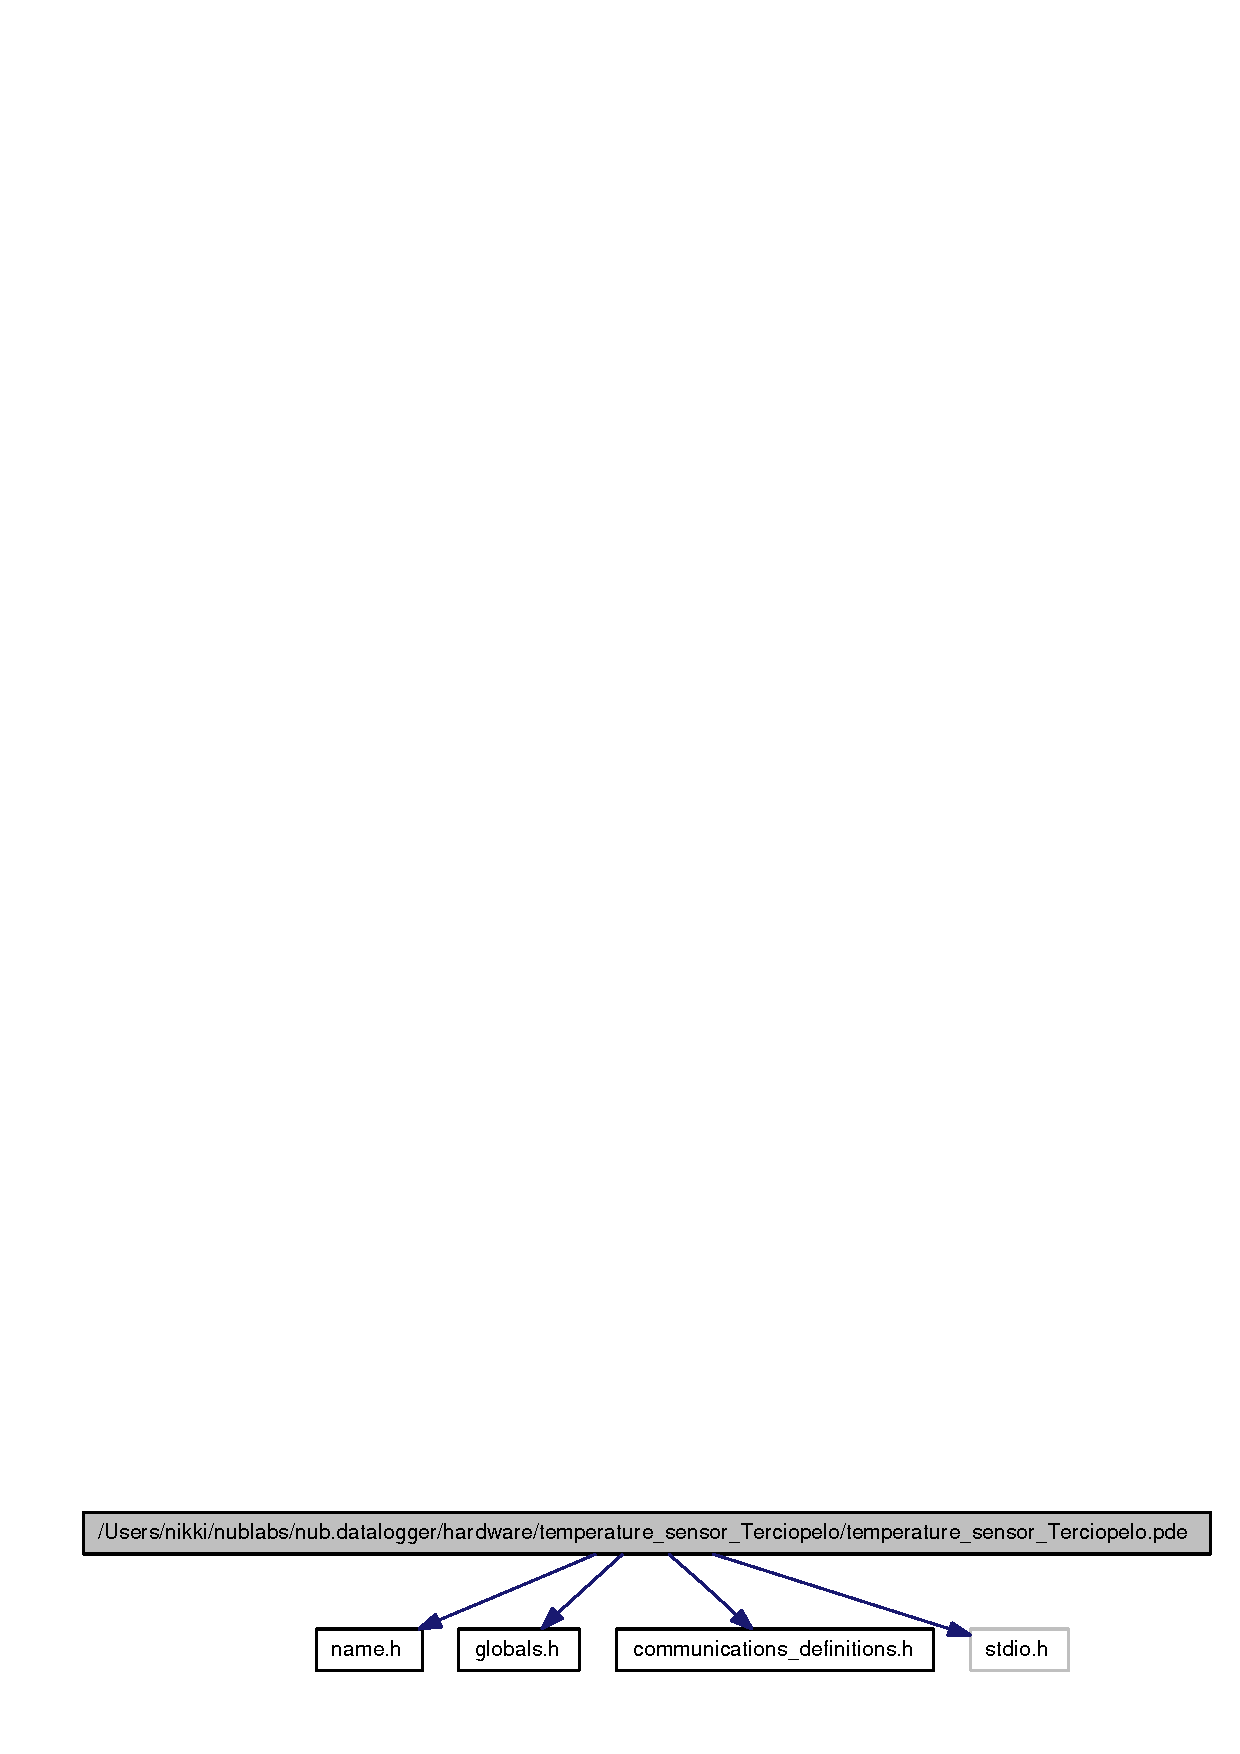
\includegraphics[width=292pt]{temperature__sensor___terciopelo_8pde__incl}
\end{center}
\end{figure}
\subsection*{Defines}
\begin{CompactItemize}
\item 
\#define \hyperlink{temperature__sensor___terciopelo_8pde_658c2878485cfe5cc625d283a6d34bc1}{XBEE\_\-SLEEP}~2
\item 
\#define \hyperlink{temperature__sensor___terciopelo_8pde_b2de299215608c2a35f0feb86adc2f6f}{SAMPLE\_\-BUTTON}~3
\item 
\#define \hyperlink{temperature__sensor___terciopelo_8pde_eb7a7ba1ab7e0406f1b5ab36d579f585}{LED}~4
\item 
\#define \hyperlink{temperature__sensor___terciopelo_8pde_2a2946288d28852ba343b09fd4f17d7a}{SENSOR1\_\-TOP}~0
\item 
\#define \hyperlink{temperature__sensor___terciopelo_8pde_0da2a51dcb3e00b10aedd07d75f22382}{SENSOR1\_\-BOTTOM}~1
\item 
\#define \hyperlink{temperature__sensor___terciopelo_8pde_645141ae2ab7fa7ac3f690c4959b6baf}{SENSOR2\_\-TOP}~2
\item 
\#define \hyperlink{temperature__sensor___terciopelo_8pde_df66e6da6cf8c78004dc0a75fd14d3b1}{SENSOR2\_\-BOTTOM}~3
\end{CompactItemize}
\subsection*{Functions}
\begin{CompactItemize}
\item 
void \hyperlink{temperature__sensor___terciopelo_8pde_4fc01d736fe50cf5b977f755b675f11d}{setup} ()
\item 
void \hyperlink{temperature__sensor___terciopelo_8pde_fe461d27b9c48d5921c00d521181f12f}{loop} ()
\item 
void \hyperlink{temperature__sensor___terciopelo_8pde_50a2ce599e896bfb535e70a42003ed23}{sample} ()
\item 
int \hyperlink{temperature__sensor___terciopelo_8pde_f8c68e93feeba5b9244094043672bac0}{getByte} (int timeout)
\item 
int \hyperlink{temperature__sensor___terciopelo_8pde_8f2521044963073c55b3c290fffd79e3}{getMessage} (int timeout)
\item 
void \hyperlink{temperature__sensor___terciopelo_8pde_95b1b253ee46df6a93285803cf1f3370}{sendData} ()
\begin{CompactList}\small\item\em this function takes care of putting together a message string, calculating a checksum, sending it out to the computer and making sure the computer got it ok \item\end{CompactList}\item 
unsigned char \hyperlink{temperature__sensor___terciopelo_8pde_465a79dc430d1e52a5b540920da744ca}{getChecksum} ()
\begin{CompactList}\small\item\em this computes a checksum of the global string 'message' \item\end{CompactList}\item 
void \hyperlink{temperature__sensor___terciopelo_8pde_e369b3765489ee8bd0ea791c1843630f}{configure} ()
\begin{CompactList}\small\item\em \hyperlink{applet_2nublogger_8h_e369b3765489ee8bd0ea791c1843630f}{configure()} runs if the computer is trying to change the sensor's sample rate \item\end{CompactList}\item 
void \hyperlink{temperature__sensor___terciopelo_8pde_3fdb2350c3f98c0de0f0ae3c831a8b14}{discover} ()
\begin{CompactList}\small\item\em This function tells the computer of the datalogger's existence. \item\end{CompactList}\item 
void \hyperlink{temperature__sensor___terciopelo_8pde_b4dbd8380e5d93ead613cf38e6083b7f}{waitForSampleInterval} ()
\begin{CompactList}\small\item\em this function waits for the time specified by the global variables 'hours,' 'minutes,' and 'seconds' It should ideally put the arduino in a power saving mode \item\end{CompactList}\item 
void \hyperlink{temperature__sensor___terciopelo_8pde_f6c9587ccbcf223f8c79f508c2fef366}{initializeSensor} ()
\begin{CompactList}\small\item\em this function configures all the digital communication pins as input or output pins \item\end{CompactList}\item 
void \hyperlink{temperature__sensor___terciopelo_8pde_a06edc5122b70b3231ff87d8234fe759}{xbeeSleep} ()
\item 
void \hyperlink{temperature__sensor___terciopelo_8pde_884c5dd8e3bb500063c819db197db666}{xbeeWake} ()
\item 
void \hyperlink{temperature__sensor___terciopelo_8pde_ea28af0c7128421a38589128bb39ef1c}{getTemperatures} ()
\item 
void \hyperlink{temperature__sensor___terciopelo_8pde_cfc975251dbc3a8c9a9b11f8df62cc41}{getRawData} ()
\begin{CompactList}\small\item\em this just grabs the raw values off the analog to digital converter \item\end{CompactList}\item 
void \hyperlink{temperature__sensor___terciopelo_8pde_8e666a34a083b1806167ca991be0c436}{convertToResistance} ()
\begin{CompactList}\small\item\em this function converts the raw ADC values from the thermistor into resistances of the thermistor \item\end{CompactList}\item 
void \hyperlink{temperature__sensor___terciopelo_8pde_3aa4f99331713009a70ee34eba83754b}{convertToTemperature} ()
\end{CompactItemize}
\subsection*{Variables}
\begin{CompactItemize}
\item 
float \hyperlink{temperature__sensor___terciopelo_8pde_735577560ca40e5b6008a98829068904}{R0} = 10000.0
\item 
float \hyperlink{temperature__sensor___terciopelo_8pde_8188fea1f6709096fe21a3ee084d00d0}{B} = 3950.0
\item 
float \hyperlink{temperature__sensor___terciopelo_8pde_4211ba1269f650e21964d32238a460b2}{T0} = 298
\item 
float \hyperlink{temperature__sensor___terciopelo_8pde_d17df5990b551ac9e97a3d60f65833ff}{RBOTTOM} = 1000.0
\end{CompactItemize}


\subsection{Define Documentation}
\hypertarget{temperature__sensor___terciopelo_8pde_eb7a7ba1ab7e0406f1b5ab36d579f585}{
\index{temperature\_\-sensor\_\-Terciopelo.pde@{temperature\_\-sensor\_\-Terciopelo.pde}!LED@{LED}}
\index{LED@{LED}!temperature_sensor_Terciopelo.pde@{temperature\_\-sensor\_\-Terciopelo.pde}}
\subsubsection[{LED}]{\setlength{\rightskip}{0pt plus 5cm}\#define LED~4}}
\label{temperature__sensor___terciopelo_8pde_eb7a7ba1ab7e0406f1b5ab36d579f585}




Definition at line 330 of file temperature\_\-sensor\_\-Terciopelo.pde.\hypertarget{temperature__sensor___terciopelo_8pde_b2de299215608c2a35f0feb86adc2f6f}{
\index{temperature\_\-sensor\_\-Terciopelo.pde@{temperature\_\-sensor\_\-Terciopelo.pde}!SAMPLE\_\-BUTTON@{SAMPLE\_\-BUTTON}}
\index{SAMPLE\_\-BUTTON@{SAMPLE\_\-BUTTON}!temperature_sensor_Terciopelo.pde@{temperature\_\-sensor\_\-Terciopelo.pde}}
\subsubsection[{SAMPLE\_\-BUTTON}]{\setlength{\rightskip}{0pt plus 5cm}\#define SAMPLE\_\-BUTTON~3}}
\label{temperature__sensor___terciopelo_8pde_b2de299215608c2a35f0feb86adc2f6f}




Definition at line 329 of file temperature\_\-sensor\_\-Terciopelo.pde.\hypertarget{temperature__sensor___terciopelo_8pde_0da2a51dcb3e00b10aedd07d75f22382}{
\index{temperature\_\-sensor\_\-Terciopelo.pde@{temperature\_\-sensor\_\-Terciopelo.pde}!SENSOR1\_\-BOTTOM@{SENSOR1\_\-BOTTOM}}
\index{SENSOR1\_\-BOTTOM@{SENSOR1\_\-BOTTOM}!temperature_sensor_Terciopelo.pde@{temperature\_\-sensor\_\-Terciopelo.pde}}
\subsubsection[{SENSOR1\_\-BOTTOM}]{\setlength{\rightskip}{0pt plus 5cm}\#define SENSOR1\_\-BOTTOM~1}}
\label{temperature__sensor___terciopelo_8pde_0da2a51dcb3e00b10aedd07d75f22382}




Definition at line 333 of file temperature\_\-sensor\_\-Terciopelo.pde.\hypertarget{temperature__sensor___terciopelo_8pde_2a2946288d28852ba343b09fd4f17d7a}{
\index{temperature\_\-sensor\_\-Terciopelo.pde@{temperature\_\-sensor\_\-Terciopelo.pde}!SENSOR1\_\-TOP@{SENSOR1\_\-TOP}}
\index{SENSOR1\_\-TOP@{SENSOR1\_\-TOP}!temperature_sensor_Terciopelo.pde@{temperature\_\-sensor\_\-Terciopelo.pde}}
\subsubsection[{SENSOR1\_\-TOP}]{\setlength{\rightskip}{0pt plus 5cm}\#define SENSOR1\_\-TOP~0}}
\label{temperature__sensor___terciopelo_8pde_2a2946288d28852ba343b09fd4f17d7a}




Definition at line 332 of file temperature\_\-sensor\_\-Terciopelo.pde.\hypertarget{temperature__sensor___terciopelo_8pde_df66e6da6cf8c78004dc0a75fd14d3b1}{
\index{temperature\_\-sensor\_\-Terciopelo.pde@{temperature\_\-sensor\_\-Terciopelo.pde}!SENSOR2\_\-BOTTOM@{SENSOR2\_\-BOTTOM}}
\index{SENSOR2\_\-BOTTOM@{SENSOR2\_\-BOTTOM}!temperature_sensor_Terciopelo.pde@{temperature\_\-sensor\_\-Terciopelo.pde}}
\subsubsection[{SENSOR2\_\-BOTTOM}]{\setlength{\rightskip}{0pt plus 5cm}\#define SENSOR2\_\-BOTTOM~3}}
\label{temperature__sensor___terciopelo_8pde_df66e6da6cf8c78004dc0a75fd14d3b1}




Definition at line 335 of file temperature\_\-sensor\_\-Terciopelo.pde.\hypertarget{temperature__sensor___terciopelo_8pde_645141ae2ab7fa7ac3f690c4959b6baf}{
\index{temperature\_\-sensor\_\-Terciopelo.pde@{temperature\_\-sensor\_\-Terciopelo.pde}!SENSOR2\_\-TOP@{SENSOR2\_\-TOP}}
\index{SENSOR2\_\-TOP@{SENSOR2\_\-TOP}!temperature_sensor_Terciopelo.pde@{temperature\_\-sensor\_\-Terciopelo.pde}}
\subsubsection[{SENSOR2\_\-TOP}]{\setlength{\rightskip}{0pt plus 5cm}\#define SENSOR2\_\-TOP~2}}
\label{temperature__sensor___terciopelo_8pde_645141ae2ab7fa7ac3f690c4959b6baf}




Definition at line 334 of file temperature\_\-sensor\_\-Terciopelo.pde.\hypertarget{temperature__sensor___terciopelo_8pde_658c2878485cfe5cc625d283a6d34bc1}{
\index{temperature\_\-sensor\_\-Terciopelo.pde@{temperature\_\-sensor\_\-Terciopelo.pde}!XBEE\_\-SLEEP@{XBEE\_\-SLEEP}}
\index{XBEE\_\-SLEEP@{XBEE\_\-SLEEP}!temperature_sensor_Terciopelo.pde@{temperature\_\-sensor\_\-Terciopelo.pde}}
\subsubsection[{XBEE\_\-SLEEP}]{\setlength{\rightskip}{0pt plus 5cm}\#define XBEE\_\-SLEEP~2}}
\label{temperature__sensor___terciopelo_8pde_658c2878485cfe5cc625d283a6d34bc1}


these are the pin definitions for the v2 board

function atmega pin arduino pin

Serial RX PD0 0 //serial lines that go out to the xbee module Serial TX PD1 1 Xbee\_\-sleep PD2 2 //a pin that, when asserted, puts the xbee radio into a low power sleep mode Sample\_\-button PD3 3 //an optional button that forces the sensor to take and send out a measurement LED PD4 4 //an LED on board that you can use for all kinds of stuff

sensor1\_\-top PC0 (analog) 0 sensor1\_\-bottom PC1 (analog) 1 sensor2\_\-top PC2 (analog) 2 sensor2\_\-bottom PC3 (analog) 3 

Definition at line 328 of file temperature\_\-sensor\_\-Terciopelo.pde.

\subsection{Function Documentation}
\hypertarget{temperature__sensor___terciopelo_8pde_e369b3765489ee8bd0ea791c1843630f}{
\index{temperature\_\-sensor\_\-Terciopelo.pde@{temperature\_\-sensor\_\-Terciopelo.pde}!configure@{configure}}
\index{configure@{configure}!temperature_sensor_Terciopelo.pde@{temperature\_\-sensor\_\-Terciopelo.pde}}
\subsubsection[{configure}]{\setlength{\rightskip}{0pt plus 5cm}void configure ()}}
\label{temperature__sensor___terciopelo_8pde_e369b3765489ee8bd0ea791c1843630f}


\hyperlink{applet_2nublogger_8h_e369b3765489ee8bd0ea791c1843630f}{configure()} runs if the computer is trying to change the sensor's sample rate 

In \hyperlink{applet_2nublogger_8h_e369b3765489ee8bd0ea791c1843630f}{configure()}, the datalogger sends a LISTENING message to the computer, indicating that it's ready to receive data. The computer sends three ints: the hours, minutes and seconds of the sample interval, followed by a checksum byte that's the sum of the ints modulo 256. The sensor computes a checksum on the received data. If its checksum matches, it sends an ACKNOWLEDGE message back to the computer and updates its sample interval information. If the checksum does not match, it sends a CHECKSUM\_\-ERROR\_\-PLEASE\_\-RESEND message, asking the computer to send the three ints again, followed by a checksum. If the sensor can't get a valid message (with a matching checksum) after three tries, it gives up, sends a CHECKSUM\_\-ERROR\_\-GIVING\_\-UP message to the computer and keeps its original sample interval information 

Definition at line 190 of file temperature\_\-sensor\_\-Terciopelo.pde.

References buffer, CHECKSUM, CHECKSUM\_\-ERROR\_\-GIVING\_\-UP, CHECKSUM\_\-ERROR\_\-PLEASE\_\-RESEND, CONFIGURATION\_\-MESSAGE\_\-LENGTH, configured, getMessage(), HOUR\_\-HIGH, HOUR\_\-LOW, hours, index, LISTENING, MALFORMED\_\-MESSAGE\_\-ERROR\_\-GIVING\_\-UP, MALFORMED\_\-MESSAGE\_\-ERROR\_\-PLEASE\_\-RESEND, MESSAGE\_\-START, MINUTE\_\-HIGH, MINUTE\_\-LOW, minutes, NUM\_\-TRIES, SECOND\_\-HIGH, SECOND\_\-LOW, seconds, start, and TIMEOUT\_\-ERROR.

\begin{Code}\begin{verbatim}191 { 
192   char i=0;
193   char tries=0;
194   char success=0;
195   unsigned char checksum=0;
196   int error;
197 
198   while((tries<NUM_TRIES)&&(success==0))     //we'll try
199   {
200     checksum=0;
201     Serial.print(LISTENING,BYTE);
202     error=getMessage(100);
203     if(error==-1)
204       Serial.print(TIMEOUT_ERROR,BYTE);
205     else
206     {
207       if(buffer[start]==MESSAGE_START)
208       {
209         if((index-start)==CONFIGURATION_MESSAGE_LENGTH)    //check to make sure the message is the size we expect
210         {
211           for(i=1;i<CHECKSUM;i++)
212             checksum+=buffer[start+i];
213           if(checksum==buffer[start+CHECKSUM])    //check to see if the calculated checksum is the same as the received checksum
214           {
215             //if it is, then we can load all the sample interval info
216             hours=(int)buffer[start+HOUR_HIGH]*256+(int)buffer[start+HOUR_LOW];
217             minutes=(int)buffer[start+MINUTE_HIGH]*256+(int)buffer[start+MINUTE_LOW];
218             seconds=(int)buffer[start+SECOND_HIGH]*256+(int)buffer[start+SECOND_LOW];
219             success=1;         //we can stop looping
220             configured=1;      //the sensor is configured!
221           }
222           else
223           {
224             if(tries<NUM_TRIES)
225             {
226               Serial.print(CHECKSUM_ERROR_PLEASE_RESEND);
227               tries++;
228             }
229             else
230               Serial.print(CHECKSUM_ERROR_GIVING_UP);
231           }
232         }
233         else      //the message is the wrong size
234         {
235           if(tries<NUM_TRIES)
236           {
237             Serial.print(MALFORMED_MESSAGE_ERROR_PLEASE_RESEND);
238             tries++;
239           }
240           else
241             Serial.print(MALFORMED_MESSAGE_ERROR_GIVING_UP);
242         }
243       }
244       else
245       {
246         if(tries<NUM_TRIES)
247         {
248           Serial.print(MALFORMED_MESSAGE_ERROR_PLEASE_RESEND);
249           tries++;
250         }
251         else
252           Serial.print(MALFORMED_MESSAGE_ERROR_GIVING_UP);
253       }
254     }
255   }
256 }
\end{verbatim}
\end{Code}


\hypertarget{temperature__sensor___terciopelo_8pde_8e666a34a083b1806167ca991be0c436}{
\index{temperature\_\-sensor\_\-Terciopelo.pde@{temperature\_\-sensor\_\-Terciopelo.pde}!convertToResistance@{convertToResistance}}
\index{convertToResistance@{convertToResistance}!temperature_sensor_Terciopelo.pde@{temperature\_\-sensor\_\-Terciopelo.pde}}
\subsubsection[{convertToResistance}]{\setlength{\rightskip}{0pt plus 5cm}void convertToResistance ()}}
\label{temperature__sensor___terciopelo_8pde_8e666a34a083b1806167ca991be0c436}


this function converts the raw ADC values from the thermistor into resistances of the thermistor 



Definition at line 390 of file temperature\_\-sensor\_\-Terciopelo.pde.

References RBOTTOM, sensor1\_\-bottom, sensor1\_\-resistance, and sensor1\_\-top.

Referenced by getTemperatures(), and sample().

\begin{Code}\begin{verbatim}391 {
392   sensor1_resistance = ((float)sensor1_top/(float)sensor1_bottom - 1)*RBOTTOM; // Voltages converted to resistances
393   /* uncomment if I enable two sensing elements
394    sensor2_resistance = ((float)sensor2_top/(float)sensor2_bottom - 1)*RBOTTOM; // Voltages converted to resistances*/
395    int a=(int) sensor1_resistance;
396    Serial.println("woohoo!");
397 //  Serial.println(a,DEC);
398 }
\end{verbatim}
\end{Code}


\hypertarget{temperature__sensor___terciopelo_8pde_3aa4f99331713009a70ee34eba83754b}{
\index{temperature\_\-sensor\_\-Terciopelo.pde@{temperature\_\-sensor\_\-Terciopelo.pde}!convertToTemperature@{convertToTemperature}}
\index{convertToTemperature@{convertToTemperature}!temperature_sensor_Terciopelo.pde@{temperature\_\-sensor\_\-Terciopelo.pde}}
\subsubsection[{convertToTemperature}]{\setlength{\rightskip}{0pt plus 5cm}void convertToTemperature ()}}
\label{temperature__sensor___terciopelo_8pde_3aa4f99331713009a70ee34eba83754b}




Definition at line 401 of file temperature\_\-sensor\_\-Terciopelo.pde.

References B, R0, sensor1\_\-resistance, sensor1\_\-temperature, and T0.

Referenced by getTemperatures(), and sample().

\begin{Code}\begin{verbatim}402 {
403   sensor1_temperature = float(B/log(sensor1_resistance/(R0*exp(-1.0*B/T0))) - 273.0); // Temperature in degrees Celsius
404   /* uncomment if I enable two sensing elements
405    sensor2_temperature = float(B/log(sensor2_resistance/(R0*exp(-1.0*B/T0))) - 273.0); // Temperature in degrees Celsius   */
406 }
\end{verbatim}
\end{Code}


\hypertarget{temperature__sensor___terciopelo_8pde_3fdb2350c3f98c0de0f0ae3c831a8b14}{
\index{temperature\_\-sensor\_\-Terciopelo.pde@{temperature\_\-sensor\_\-Terciopelo.pde}!discover@{discover}}
\index{discover@{discover}!temperature_sensor_Terciopelo.pde@{temperature\_\-sensor\_\-Terciopelo.pde}}
\subsubsection[{discover}]{\setlength{\rightskip}{0pt plus 5cm}void discover ()}}
\label{temperature__sensor___terciopelo_8pde_3fdb2350c3f98c0de0f0ae3c831a8b14}


This function tells the computer of the datalogger's existence. 

When the sensor turns on, it runs \hyperlink{applet_2nublogger_8h_3fdb2350c3f98c0de0f0ae3c831a8b14}{discover()}. It sends a MESSAGE\_\-START message, a DISCOVER\_\-ME message, and its name out to the computer and waits for acknowledgement. The computer can send back a plain \char`\"{}ACKNOWLEDGE\char`\"{} message, which means that the sensor should run using its default configuration values. The computer can also send back an \char`\"{}ACKNOWLEDGE\_\-AND\_\-CONFIGURE\char`\"{} message, which means that it has configuration data for the sensor. If the sensor gets this message, it'll run \hyperlink{applet_2nublogger_8h_e369b3765489ee8bd0ea791c1843630f}{configure()} to receive the data from the computer. 

Definition at line 267 of file temperature\_\-sensor\_\-Terciopelo.pde.

References ACKNOWLEDGE, ACKNOWLEDGE\_\-AND\_\-CONFIGURE, configure(), DISCOVER\_\-ME, discovered, getByte(), MESSAGE\_\-END, MESSAGE\_\-START, name, TIMEOUT\_\-ERROR, and TRUE.

\begin{Code}\begin{verbatim}268 { 
269   unsigned char checksum=0;
270   int i=0;
271   Serial.print(MESSAGE_START, BYTE);
272   Serial.print(DISCOVER_ME,BYTE);
273   Serial.print(name);
274   while(name[i]!=0)
275   {
276     checksum+=name[i];
277     i++;
278   }
279   checksum+=DISCOVER_ME;
280   Serial.print(checksum,BYTE);
281   Serial.print(MESSAGE_END,BYTE);
282 
283   int receivedByte=getByte(100);     //looks for a byte on the serial port with a 100ms timeout
284   if(receivedByte==ACKNOWLEDGE)
285     discovered=TRUE;
286   if(receivedByte==ACKNOWLEDGE_AND_CONFIGURE)
287   {
288     discovered=TRUE;
289     configure();
290   }
291   if(receivedByte==-1)
292   {
293     Serial.print(TIMEOUT_ERROR,BYTE);  //getByte didn't get a byte before the timeout
294   }  
295 }
\end{verbatim}
\end{Code}


\hypertarget{temperature__sensor___terciopelo_8pde_f8c68e93feeba5b9244094043672bac0}{
\index{temperature\_\-sensor\_\-Terciopelo.pde@{temperature\_\-sensor\_\-Terciopelo.pde}!getByte@{getByte}}
\index{getByte@{getByte}!temperature_sensor_Terciopelo.pde@{temperature\_\-sensor\_\-Terciopelo.pde}}
\subsubsection[{getByte}]{\setlength{\rightskip}{0pt plus 5cm}int getByte (int {\em timeout})}}
\label{temperature__sensor___terciopelo_8pde_f8c68e93feeba5b9244094043672bac0}




Definition at line 96 of file temperature\_\-sensor\_\-Terciopelo.pde.

\begin{Code}\begin{verbatim}97 {
98   unsigned long currentTime=millis();
99   unsigned long maxTime=currentTime+timeout;
100   while((Serial.available()==0)&&(millis()<(maxTime)))
101   {
102   }
103   if(Serial.available()>0)        //did any data come in on the serial port?
104     return Serial.read();
105   else                             //we didn't get any data before the timeout
106   return -1;
107 }
\end{verbatim}
\end{Code}


\hypertarget{temperature__sensor___terciopelo_8pde_465a79dc430d1e52a5b540920da744ca}{
\index{temperature\_\-sensor\_\-Terciopelo.pde@{temperature\_\-sensor\_\-Terciopelo.pde}!getChecksum@{getChecksum}}
\index{getChecksum@{getChecksum}!temperature_sensor_Terciopelo.pde@{temperature\_\-sensor\_\-Terciopelo.pde}}
\subsubsection[{getChecksum}]{\setlength{\rightskip}{0pt plus 5cm}unsigned char getChecksum ()}}
\label{temperature__sensor___terciopelo_8pde_465a79dc430d1e52a5b540920da744ca}


this computes a checksum of the global string 'message' 



Definition at line 166 of file temperature\_\-sensor\_\-Terciopelo.pde.

References message.

Referenced by sendData().

\begin{Code}\begin{verbatim}167 {
168   char i=0;
169   unsigned char checksum=0;
170   while(message[i]!=0)
171   {
172     checksum+=message[i];
173     i++;
174   }
175   return checksum;
176 }
\end{verbatim}
\end{Code}


\hypertarget{temperature__sensor___terciopelo_8pde_8f2521044963073c55b3c290fffd79e3}{
\index{temperature\_\-sensor\_\-Terciopelo.pde@{temperature\_\-sensor\_\-Terciopelo.pde}!getMessage@{getMessage}}
\index{getMessage@{getMessage}!temperature_sensor_Terciopelo.pde@{temperature\_\-sensor\_\-Terciopelo.pde}}
\subsubsection[{getMessage}]{\setlength{\rightskip}{0pt plus 5cm}int getMessage (int {\em timeout})}}
\label{temperature__sensor___terciopelo_8pde_8f2521044963073c55b3c290fffd79e3}




Definition at line 109 of file temperature\_\-sensor\_\-Terciopelo.pde.

References buffer, index, MESSAGE\_\-END, and start.

Referenced by configure().

\begin{Code}\begin{verbatim}110 {
111   int completeMessage=-1;   //a flag that lets us know if we got a full message
112   start=index;              //drop whatever other data is in our buffer--it'll probably just confuse the functions if we don't
113   int currentTime=millis();
114   int maxTime=currentTime+timeout;  
115   while((millis()<(maxTime))&&(buffer[index]!=MESSAGE_END))
116   {
117     if(Serial.available()>0)
118     {
119       buffer[index]=Serial.read();
120       if(buffer[index]==MESSAGE_END)   //we got a complete message
121         completeMessage=1;
122       index++;
123     }
124   }
125   if(completeMessage==-1)    //we never got a complete message
126     start=index;    //skip past whatever we got from the buffer
127 
128   return completeMessage;
129 }
\end{verbatim}
\end{Code}


\hypertarget{temperature__sensor___terciopelo_8pde_cfc975251dbc3a8c9a9b11f8df62cc41}{
\index{temperature\_\-sensor\_\-Terciopelo.pde@{temperature\_\-sensor\_\-Terciopelo.pde}!getRawData@{getRawData}}
\index{getRawData@{getRawData}!temperature_sensor_Terciopelo.pde@{temperature\_\-sensor\_\-Terciopelo.pde}}
\subsubsection[{getRawData}]{\setlength{\rightskip}{0pt plus 5cm}void getRawData ()}}
\label{temperature__sensor___terciopelo_8pde_cfc975251dbc3a8c9a9b11f8df62cc41}


this just grabs the raw values off the analog to digital converter 



Definition at line 379 of file temperature\_\-sensor\_\-Terciopelo.pde.

References sensor1\_\-bottom, and sensor1\_\-top.

Referenced by getTemperatures(), and sample().

\begin{Code}\begin{verbatim}380 {
381   sensor1_top=analogRead(0);
382   sensor1_bottom=analogRead(1);
383 
384   /*  uncomment if I enable 2-sensing elements per sensor
385    sensor2_top=analogRead(2);
386    sensor2_bottom=analogRead(3);*/
387 }
\end{verbatim}
\end{Code}


\hypertarget{temperature__sensor___terciopelo_8pde_ea28af0c7128421a38589128bb39ef1c}{
\index{temperature\_\-sensor\_\-Terciopelo.pde@{temperature\_\-sensor\_\-Terciopelo.pde}!getTemperatures@{getTemperatures}}
\index{getTemperatures@{getTemperatures}!temperature_sensor_Terciopelo.pde@{temperature\_\-sensor\_\-Terciopelo.pde}}
\subsubsection[{getTemperatures}]{\setlength{\rightskip}{0pt plus 5cm}void getTemperatures ()}}
\label{temperature__sensor___terciopelo_8pde_ea28af0c7128421a38589128bb39ef1c}




Definition at line 371 of file temperature\_\-sensor\_\-Terciopelo.pde.

References convertToResistance(), convertToTemperature(), and getRawData().

\begin{Code}\begin{verbatim}372 {
373   getRawData();
374   convertToResistance();
375   convertToTemperature();
376 }
\end{verbatim}
\end{Code}


\hypertarget{temperature__sensor___terciopelo_8pde_f6c9587ccbcf223f8c79f508c2fef366}{
\index{temperature\_\-sensor\_\-Terciopelo.pde@{temperature\_\-sensor\_\-Terciopelo.pde}!initializeSensor@{initializeSensor}}
\index{initializeSensor@{initializeSensor}!temperature_sensor_Terciopelo.pde@{temperature\_\-sensor\_\-Terciopelo.pde}}
\subsubsection[{initializeSensor}]{\setlength{\rightskip}{0pt plus 5cm}void initializeSensor ()}}
\label{temperature__sensor___terciopelo_8pde_f6c9587ccbcf223f8c79f508c2fef366}


this function configures all the digital communication pins as input or output pins 

If you adapt this code to work with another sensor or board, you should replace the code in \hyperlink{applet_2temperature__sensor__board__v2_8h_f6c9587ccbcf223f8c79f508c2fef366}{initializeSensor()} to initialize all your relevant pins 

Definition at line 350 of file temperature\_\-sensor\_\-Terciopelo.pde.

References LED, SAMPLE\_\-BUTTON, XBEE\_\-SLEEP, and xbeeWake().

\begin{Code}\begin{verbatim}351 {
352   pinMode(XBEE_SLEEP,OUTPUT);
353   pinMode(SAMPLE_BUTTON,INPUT);
354   pinMode(LED,OUTPUT);
355   xbeeWake();
356 }  
\end{verbatim}
\end{Code}


\hypertarget{temperature__sensor___terciopelo_8pde_fe461d27b9c48d5921c00d521181f12f}{
\index{temperature\_\-sensor\_\-Terciopelo.pde@{temperature\_\-sensor\_\-Terciopelo.pde}!loop@{loop}}
\index{loop@{loop}!temperature_sensor_Terciopelo.pde@{temperature\_\-sensor\_\-Terciopelo.pde}}
\subsubsection[{loop}]{\setlength{\rightskip}{0pt plus 5cm}void loop ()}}
\label{temperature__sensor___terciopelo_8pde_fe461d27b9c48d5921c00d521181f12f}




Definition at line 79 of file temperature\_\-sensor\_\-Terciopelo.pde.

References sample(), and waitForSampleInterval().

Referenced by main().

\begin{Code}\begin{verbatim}80 {
81   waitForSampleInterval();
82   sample();
83 }
\end{verbatim}
\end{Code}


\hypertarget{temperature__sensor___terciopelo_8pde_50a2ce599e896bfb535e70a42003ed23}{
\index{temperature\_\-sensor\_\-Terciopelo.pde@{temperature\_\-sensor\_\-Terciopelo.pde}!sample@{sample}}
\index{sample@{sample}!temperature_sensor_Terciopelo.pde@{temperature\_\-sensor\_\-Terciopelo.pde}}
\subsubsection[{sample}]{\setlength{\rightskip}{0pt plus 5cm}void sample ()}}
\label{temperature__sensor___terciopelo_8pde_50a2ce599e896bfb535e70a42003ed23}




Definition at line 85 of file temperature\_\-sensor\_\-Terciopelo.pde.

References convertToResistance(), convertToTemperature(), getRawData(), sampleNumber, and sendData().

Referenced by loop().

\begin{Code}\begin{verbatim}86 {
87   getRawData();
88   convertToResistance();
89   convertToTemperature();
90   sendData();
91   sampleNumber++;
92 }
\end{verbatim}
\end{Code}


\hypertarget{temperature__sensor___terciopelo_8pde_95b1b253ee46df6a93285803cf1f3370}{
\index{temperature\_\-sensor\_\-Terciopelo.pde@{temperature\_\-sensor\_\-Terciopelo.pde}!sendData@{sendData}}
\index{sendData@{sendData}!temperature_sensor_Terciopelo.pde@{temperature\_\-sensor\_\-Terciopelo.pde}}
\subsubsection[{sendData}]{\setlength{\rightskip}{0pt plus 5cm}void sendData ()}}
\label{temperature__sensor___terciopelo_8pde_95b1b253ee46df6a93285803cf1f3370}


this function takes care of putting together a message string, calculating a checksum, sending it out to the computer and making sure the computer got it ok 



Definition at line 133 of file temperature\_\-sensor\_\-Terciopelo.pde.

References ACKNOWLEDGE, ACKNOWLEDGE\_\-AND\_\-CONFIGURE, configure(), FALSE, getByte(), getChecksum(), message, MESSAGE\_\-END, MESSAGE\_\-START, NUM\_\-TRIES, sampleNumber, sensor1\_\-temperature, and TRUE.

Referenced by sample().

\begin{Code}\begin{verbatim}134 {
135   char tries=0;
136   char success=FALSE;
137   int sensor1_temperature_decimals=(sensor1_temperature-(int)sensor1_temperature)*100;    //sprintf doesn't work for floats, so this hack gets 2 sigfigs
138   int response=0;
139  // sprintf(message,"%d", sampleNumber);
140   sprintf(message, " %d thermistor 1 = %d.%d degrees C", sampleNumber, (int)sensor1_temperature, sensor1_temperature_decimals);
141 //sprintf(message,"%d %d %d", (int) sensor1_temperature, (int) sensor1_resistance, sensor1_temperature_decimals);
142   unsigned char checksum=getChecksum();
143   while((success==FALSE)&&(tries<NUM_TRIES))
144   {
145     Serial.print(MESSAGE_START,BYTE);
146     Serial.print(message);
147     Serial.print(checksum);
148     Serial.print(MESSAGE_END,BYTE);
149     response=getByte(50);   //look for the computer's response
150 
151     if(response==ACKNOWLEDGE)   //the computer got the data.  It's happy, we're happy, we're done!
152       success=TRUE;
153 
154     else if(response==ACKNOWLEDGE_AND_CONFIGURE)  //the computer can ask to upload a new configuration at any sample
155     {
156       success=TRUE;
157       configure();
158     }
159     else         //if there was a timeout or a checksum mismatch, then re-try
160     tries++;
161   }
162 
163 }
\end{verbatim}
\end{Code}


\hypertarget{temperature__sensor___terciopelo_8pde_4fc01d736fe50cf5b977f755b675f11d}{
\index{temperature\_\-sensor\_\-Terciopelo.pde@{temperature\_\-sensor\_\-Terciopelo.pde}!setup@{setup}}
\index{setup@{setup}!temperature_sensor_Terciopelo.pde@{temperature\_\-sensor\_\-Terciopelo.pde}}
\subsubsection[{setup}]{\setlength{\rightskip}{0pt plus 5cm}void setup ()}}
\label{temperature__sensor___terciopelo_8pde_4fc01d736fe50cf5b977f755b675f11d}


nublogger temperature sensor Terciopelo(+)

Alex Hornstein 11.19.08 \href{mailto:alex@nublabs.com}{\tt alex@nublabs.com} datalogger.nublabs.com

(+)In keeping with the arduino nomenclature, we are naming all our code revisions with Spanish names of venemous snakes. The Terciopelo, or fer-de-lance is a pit viper common in central and northwestern south america. It has a powerful venom that, left untreated, can cause necrosis, brain hemorrhaging, renal failure and death. It's also capable of spraying venom through its fangs for up to 6 feet. Cool, huh? This is a sensor for nublab's datalogging system. The datalogger is a two-part system: There is a USB dongle that plugs into a computer that allows the computer to talk to a wireless Zigbee network, and then there are battery-powered sensors that sense data about the environemnt. The sensors collect data and convert it into human-readable units, and then send the data as plaintext over the wireless network to the computer, where it is stored and logged. Any sensor that will work with this system must implement the \hyperlink{applet_2nublogger_8h_3fdb2350c3f98c0de0f0ae3c831a8b14}{discover()}, \hyperlink{applet_2nublogger_8h_e369b3765489ee8bd0ea791c1843630f}{configure()} and \hyperlink{temperature__sensor___terciopelo_8cpp_50a2ce599e896bfb535e70a42003ed23}{sample()} functions, as well as be identifiable by a unique name

The \hyperlink{applet_2nublogger_8h_3fdb2350c3f98c0de0f0ae3c831a8b14}{discover()} function is a short communication sequence when the sensor is first turned on where it broadcasts its name over the network and ensures that the computer recognizes it and is ready to configure it and log its data. The sensor also sends the units of whatever value it will be reporting.

the \hyperlink{applet_2nublogger_8h_e369b3765489ee8bd0ea791c1843630f}{configure()} function is triggered by a flag sent by the computer that indicates that the computer would like to change the datalogger's sample rate. \hyperlink{applet_2nublogger_8h_e369b3765489ee8bd0ea791c1843630f}{configure()} is another communication sequence in which the computer sends a sample interval in hours, minutes and seconds to the datalogger. By default, the datalogger samples every second.

the \hyperlink{temperature__sensor___terciopelo_8cpp_50a2ce599e896bfb535e70a42003ed23}{sample()} function is called by the sensor every sample interval. \hyperlink{temperature__sensor___terciopelo_8cpp_50a2ce599e896bfb535e70a42003ed23}{sample()} reads a value from whatever sensing element (Thermistor, current sensor, light sensor, etc) the particular sensor uses, converts it to physical units (degrees celsius, amps, lux, etc) and sends out a string over the wireless network with the sensor's unique name and its sensed values.

the name: each sensor should have a unique name burnt into its eeprom that makes it uniquely identifiable in the network. Nublabs is using a list of north and south american baby names which is available at datalogger.nublabs.com This particular sensor is a temperature sensor using an NTC thermistor. The thermistor is a resistive element. We sense it using two resistor dividers--one resistor, R1 which connects from Vcc to the thermistor, and another resistor that connects from the other end of the thermistor to ground. We measure the voltage at both ends of the thermistor using separate Analog to Digital Converter (ADC) pins. This allows us to factor out any effect changing battery voltage has on our temperature measurement. This code is written for version 2 of the sensor hardware. A pdf of the sensor schematic and board layout is available at datalogger.nublabs.com 

Definition at line 72 of file temperature\_\-sensor\_\-Terciopelo.pde.

References discover(), and initializeSensor().

Referenced by main().

\begin{Code}\begin{verbatim}73 {
74   Serial.begin(19200);
75   initializeSensor();
76   discover();
77 }
\end{verbatim}
\end{Code}


\hypertarget{temperature__sensor___terciopelo_8pde_b4dbd8380e5d93ead613cf38e6083b7f}{
\index{temperature\_\-sensor\_\-Terciopelo.pde@{temperature\_\-sensor\_\-Terciopelo.pde}!waitForSampleInterval@{waitForSampleInterval}}
\index{waitForSampleInterval@{waitForSampleInterval}!temperature_sensor_Terciopelo.pde@{temperature\_\-sensor\_\-Terciopelo.pde}}
\subsubsection[{waitForSampleInterval}]{\setlength{\rightskip}{0pt plus 5cm}void waitForSampleInterval ()}}
\label{temperature__sensor___terciopelo_8pde_b4dbd8380e5d93ead613cf38e6083b7f}


this function waits for the time specified by the global variables 'hours,' 'minutes,' and 'seconds' It should ideally put the arduino in a power saving mode 



Definition at line 299 of file temperature\_\-sensor\_\-Terciopelo.pde.

References minutes, seconds, xbeeSleep(), and xbeeWake().

Referenced by loop().

\begin{Code}\begin{verbatim}300 {
301   xbeeSleep();
302   delay(60*minutes*1000+seconds*1000);
303   xbeeWake();
304 }
\end{verbatim}
\end{Code}


\hypertarget{temperature__sensor___terciopelo_8pde_a06edc5122b70b3231ff87d8234fe759}{
\index{temperature\_\-sensor\_\-Terciopelo.pde@{temperature\_\-sensor\_\-Terciopelo.pde}!xbeeSleep@{xbeeSleep}}
\index{xbeeSleep@{xbeeSleep}!temperature_sensor_Terciopelo.pde@{temperature\_\-sensor\_\-Terciopelo.pde}}
\subsubsection[{xbeeSleep}]{\setlength{\rightskip}{0pt plus 5cm}void xbeeSleep ()}}
\label{temperature__sensor___terciopelo_8pde_a06edc5122b70b3231ff87d8234fe759}




Definition at line 359 of file temperature\_\-sensor\_\-Terciopelo.pde.

References XBEE\_\-SLEEP.

Referenced by waitForSampleInterval().

\begin{Code}\begin{verbatim}360 {
361   digitalWrite(XBEE_SLEEP,HIGH);
362 }
\end{verbatim}
\end{Code}


\hypertarget{temperature__sensor___terciopelo_8pde_884c5dd8e3bb500063c819db197db666}{
\index{temperature\_\-sensor\_\-Terciopelo.pde@{temperature\_\-sensor\_\-Terciopelo.pde}!xbeeWake@{xbeeWake}}
\index{xbeeWake@{xbeeWake}!temperature_sensor_Terciopelo.pde@{temperature\_\-sensor\_\-Terciopelo.pde}}
\subsubsection[{xbeeWake}]{\setlength{\rightskip}{0pt plus 5cm}void xbeeWake ()}}
\label{temperature__sensor___terciopelo_8pde_884c5dd8e3bb500063c819db197db666}




Definition at line 365 of file temperature\_\-sensor\_\-Terciopelo.pde.

References XBEE\_\-SLEEP.

Referenced by initializeSensor(), and waitForSampleInterval().

\begin{Code}\begin{verbatim}366 {
367   digitalWrite(XBEE_SLEEP,LOW);
368 }
\end{verbatim}
\end{Code}




\subsection{Variable Documentation}
\hypertarget{temperature__sensor___terciopelo_8pde_8188fea1f6709096fe21a3ee084d00d0}{
\index{temperature\_\-sensor\_\-Terciopelo.pde@{temperature\_\-sensor\_\-Terciopelo.pde}!B@{B}}
\index{B@{B}!temperature_sensor_Terciopelo.pde@{temperature\_\-sensor\_\-Terciopelo.pde}}
\subsubsection[{B}]{\setlength{\rightskip}{0pt plus 5cm}float {\bf B} = 3950.0}}
\label{temperature__sensor___terciopelo_8pde_8188fea1f6709096fe21a3ee084d00d0}




Definition at line 339 of file temperature\_\-sensor\_\-Terciopelo.pde.\hypertarget{temperature__sensor___terciopelo_8pde_735577560ca40e5b6008a98829068904}{
\index{temperature\_\-sensor\_\-Terciopelo.pde@{temperature\_\-sensor\_\-Terciopelo.pde}!R0@{R0}}
\index{R0@{R0}!temperature_sensor_Terciopelo.pde@{temperature\_\-sensor\_\-Terciopelo.pde}}
\subsubsection[{R0}]{\setlength{\rightskip}{0pt plus 5cm}float {\bf R0} = 10000.0}}
\label{temperature__sensor___terciopelo_8pde_735577560ca40e5b6008a98829068904}




Definition at line 338 of file temperature\_\-sensor\_\-Terciopelo.pde.\hypertarget{temperature__sensor___terciopelo_8pde_d17df5990b551ac9e97a3d60f65833ff}{
\index{temperature\_\-sensor\_\-Terciopelo.pde@{temperature\_\-sensor\_\-Terciopelo.pde}!RBOTTOM@{RBOTTOM}}
\index{RBOTTOM@{RBOTTOM}!temperature_sensor_Terciopelo.pde@{temperature\_\-sensor\_\-Terciopelo.pde}}
\subsubsection[{RBOTTOM}]{\setlength{\rightskip}{0pt plus 5cm}float {\bf RBOTTOM} = 1000.0}}
\label{temperature__sensor___terciopelo_8pde_d17df5990b551ac9e97a3d60f65833ff}




Definition at line 341 of file temperature\_\-sensor\_\-Terciopelo.pde.\hypertarget{temperature__sensor___terciopelo_8pde_4211ba1269f650e21964d32238a460b2}{
\index{temperature\_\-sensor\_\-Terciopelo.pde@{temperature\_\-sensor\_\-Terciopelo.pde}!T0@{T0}}
\index{T0@{T0}!temperature_sensor_Terciopelo.pde@{temperature\_\-sensor\_\-Terciopelo.pde}}
\subsubsection[{T0}]{\setlength{\rightskip}{0pt plus 5cm}float {\bf T0} = 298}}
\label{temperature__sensor___terciopelo_8pde_4211ba1269f650e21964d32238a460b2}




Definition at line 340 of file temperature\_\-sensor\_\-Terciopelo.pde.
\printindex
\end{document}
